\documentclass[12pt,english]{article}
\usepackage[a4paper,left=3cm,right=2cm,top=2.5cm,bottom=2.5cm]{geometry}
\usepackage[utf8]{inputenc}
\usepackage[english]{babel}
\usepackage{graphicx}
\usepackage{pifont}
\usepackage{color}
\usepackage{xcolor}
\usepackage{colortbl}
\usepackage{amsthm,thmtools}
\usepackage{multirow}
\usepackage{pgfgantt}
\usepackage{amsmath}
\usepackage{subcaption}
\usepackage{booktabs}
\usepackage{adjustbox}
\usepackage{url}
\usepackage{svg}
\newcommand{\back}[1]{\fontsize{60}{70}\selectfont #1}
\usepackage{multirow}
\usepackage[hidelinks]{hyperref}
\usepackage{caption}
\usepackage{apacite}
\definecolor{swotS}{RGB}{226,237,143}
\definecolor{swotW}{RGB}{247,193,139}
\definecolor{swotO}{RGB}{173,208,187}
\definecolor{swotT}{RGB}{192,165,184}
\usepackage{eurosym} % para el euro
\usepackage[raster]{tcolorbox}
\usepackage{amsthm}
\usepackage{multicol}
\usepackage{float}
\usepackage{amsfonts}
\usepackage[usestackEOL]{stackengine}
\usepackage{titling}
\usepackage{soul}
\usepackage{dirtree}
\usepackage{pgfplots}
\usepackage[nottoc]{tocbibind}
\usepackage{listings}
\usepackage{array}
\usepackage[framemethod=tikz]{mdframed}
\usetikzlibrary{matrix}
\usepackage{footnote}
\newcommand{\dollar}{\mbox{\textdollar}}
\usepackage{lscape}
\usepackage{amsmath}  % for \hookrightarrow
\usepackage{xcolor}   % for \textcolor
\usepackage{incgraph}
\makesavenoteenv{tabular}
\makesavenoteenv{table}
\newcommand{\greentick}{\textcolor{green}{\ding{52}}}
\newcommand{\redcross}{\textcolor{red}{\ding{55}}}
\graphicspath{ {./img/}}
\makeatletter
\def\input@path{{input/}}
\makeatother
\selectlanguage{english}
%\usepackage{fancyhdr}
%\pagestyle{fancy}
\usepackage[
    type={CC},
    modifier={by-nc-sa},
    version={4.0},
]{doclicense}
% Default fixed font does not support bold face
\DeclareFixedFont{\ttb}{T1}{txtt}{bx}{n}{10} % for bold
\DeclareFixedFont{\ttm}{T1}{txtt}{m}{n}{10}  % for normal

% Custom colors
\usepackage{color}
\definecolor{deepblue}{rgb}{0,0,0.5}
\definecolor{deepred}{rgb}{0.6,0,0}
\definecolor{deepgreen}{rgb}{0,0.5,0}
% Python style for highlighting
\newcommand\pythonstyle{\lstset{
language=Python,
basicstyle=\ttm,
otherkeywords={self},             % Add keywords here
keywordstyle=\ttb\color{deepblue},
emph={MyClass,__init__},          % Custom highlighting
emphstyle=\ttb\color{deepred},    % Custom highlighting style
stringstyle=\color{deepgreen},
frame=tb,                         % Any extra options here
showstringspaces=false            %
}}
% Python environment
\lstnewenvironment{python}[1][]
{
\pythonstyle
\lstset{#1}
}
{}

% Python for external files
\newcommand\pythonexternal[2][]{{
\pythonstyle
\lstinputlisting[#1]{#2}}}

% Python for inline
\newcommand\pythoninline[1]{{\pythonstyle\lstinline!#1!}}

\colorlet{helpful}{lime!70}
\colorlet{harmful}{red!30}
\colorlet{internal}{yellow!20}
\colorlet{external}{cyan!30}
\colorlet{S}{helpful!50!internal}
\colorlet{W}{harmful!50!internal}
\colorlet{O}{helpful!50!external}
\colorlet{T}{harmful!50!external}

\lstset{
  breaklines=true,
  postbreak=\mbox{\textcolor{red}{$\hookrightarrow$}\space},
  mathescape = true,
  basicstyle=\ttm,
  keywordstyle=\ttb\color{deepblue},
  emph={MyClass,__init__},          % Custom highlighting
  emphstyle=\ttb\color{deepred},    % Custom highlighting style
  stringstyle=\color{deepgreen},
  frame=tb,                         % Any extra options here
  showstringspaces=false,            %
  aboveskip=20pt,
  belowskip=20pt
}

\lstdefinelanguage{docker}{
  keywords={FROM, RUN, COPY, ADD, ENTRYPOINT, CMD,  ENV, ARG, WORKDIR, EXPOSE, LABEL, USER, VOLUME, STOPSIGNAL, ONBUILD, MAINTAINER},
  keywordstyle=\color{blue}\bfseries,
  identifierstyle=\color{black},
  sensitive=false,
  comment=[l]{\#},
  commentstyle=\color{purple}\ttfamily,
  stringstyle=\color{red}\ttfamily,
  morestring=[b]',
  morestring=[b]"
}

\lstdefinelanguage{docker-compose}{
  keywords={image, environment, ports, container_name, ports, volumes, links},
  keywordstyle=\color{blue}\bfseries,
  identifierstyle=\color{black},
  sensitive=false,
  comment=[l]{\#},
  commentstyle=\color{purple}\ttfamily,
  stringstyle=\color{red}\ttfamily,
  morestring=[b]',
  morestring=[b]"
}
\lstdefinelanguage{nginx}{
  keywords={server},
  keywordstyle=[2]\color{blue}\bfseries,
  keywordstyle=[3]\color{purple}\ttfamily,
  keywords=[2]{listen, location},
  keywords=[3]{proxy_pass, proxy_set_header},
  keywordstyle=\color{olive}\bfseries,
  identifierstyle=\color{black},
  sensitive=false,
  comment=[l]{\#},
  commentstyle=\color{purple}\ttfamily,
  stringstyle=\color{red}\ttfamily,
  morestring=[b]',
  morestring=[b]"
}
\lstdefinelanguage{docker-compose-2}{
  keywords={version, services},
  keywordstyle=[2]\color{blue}\bfseries,
  keywords=[2]{image, environment, ports, container_name, ports, links, build,
  volumes, depends_on, restart},
  keywordstyle=\color{olive}\bfseries,
  identifierstyle=\color{black},
  sensitive=false,
  comment=[l]{\#},
  commentstyle=\color{purple}\ttfamily,
  stringstyle=\color{red}\ttfamily,
  morestring=[b]',
  morestring=[b]"
}

\makeindex

\definecolor{light-gray}{gray}{0.95}
\lstset{columns=fullflexible,basicstyle=\ttfamily}
\newcommand{\texta}{Helpful\\ \tiny (to achieve the objective)\par}
\newcommand{\textb}{Harmful\\ \tiny (to achieve the objective)\par}
\newcommand{\textcn}{Internal origin\\ \tiny (product\slash company attributes)\par}
\newcommand{\textdn}{External origin\\ \tiny (environment\slash market attributes)\par}


\pgfplotsset{width=8cm,compat=1.9, xlabel={Year},
  ylabel={Number of documents}, xtick distance={2},
  ytick distance={2}, ymajorgrids=true,grid style=dashed,
  /pgf/number format/.cd,use comma,1000 sep={}}


\begin{document}

\begin{titlepage}

 \newlength{\centeroffset}
 \setlength{\centeroffset}{-0.5\oddsidemargin}
 \addtolength{\centeroffset}{0.5\evensidemargin}
 \thispagestyle{empty}

 \noindent\hspace*{\centeroffset}
 \begin{minipage}{\textwidth}

  \centering
  
\includegraphics[width=0.9\textwidth]{logo_ugr.jpg}\\[1.4cm]

  \textsc{ \Large Bachelor Final Project\\[0.2cm]}
  \textsc{Computer Engineering}\\[1cm]

  {\Huge\bfseries HOW-R-U?\\}
  \noindent\rule[-1ex]{\textwidth}{3pt}\\[3.5ex]
  {\large\bfseries Analising chatbot messages to automatically infer human behaviour}
 \end{minipage}

 \vspace{1cm}
 \noindent\hspace*{\centeroffset}
 \begin{minipage}{\textwidth}
  \centering

  \textbf{Author}\\ {Carlos Sánchez Páez}\\[2.5ex]
  \textbf{Supervisor}\\
  {Oresti Baños Legrán}\\[3ex]
  
\includegraphics[width=0.4\textwidth]{etsiit_logo.png}\\[0.1cm]
  \vspace{2.5ex}
  
\includegraphics[width=0.15\textwidth]{atc.jpg}\\[0.1cm]
  \vspace{1cm}
  \textsc{Escuela Técnica Superior de Ingenierías Informática y de Telecomunicación}\\
  \vspace{1cm}
  \textsc{Granada, academic year 2019-2020}
 \end{minipage}
\end{titlepage}


\cleardoublepage
\thispagestyle{empty}

\begin{center}
{\large\bfseries  HOW-R-U?: Suite of e-coaches aimed to analyse human behaviour}\\
\end{center}
\begin{center}
Carlos Sánchez Páez\\
\end{center}

%\vspace{0.7cm}
\noindent{\textbf{Palabras clave}: chatbot, telegram, salud, médico, asistente, coach, suite}\\

\vspace{0.7cm}
\noindent{\textbf{Resumen}}\\

Hoy en día los trastornos mentales siguen siendo difíciles de tratar y diagnosticar. Además, debido al estigma que conllevan, algunos de los posibles pacientes no se sienten cómodos acudiendo a un profesional de la psicología. El objetivo de este proyecto es desarrollar una suite de e-coaches en forma de chatbots, específicamente, un chatbot de salud mental que ayude al diagnóstico prematuro de enfermedades mentales como la ansiedad y la depresión. Esta suite será modular, de forma que cada especialista pueda tener un agente conversacional asociado (psicólogo, nutricionista, etc.). Además, se le incorporará funcionalidad para que sea útil no solo para doctores, sino para analistas de datos, que contarán con la información recopilada de todos los pacientes.\\

Se plantea como trabajo futuro el uso de este sistema en un entorno en el que el asistente iniciará una conversación regularmente con el paciente y le hará una serie de preguntas definidas por su doctor. Tras ello, el especialista podrá acceder a una interfaz web en la que consultará y analizará las distintas respuestas proporcionadas por el paciente.
\cleardoublepage


\thispagestyle{empty}


\begin{center}
{\large\bfseries HOW-R-U?: Suite of e-coaches aimed to analyse human behaviour}\\
\end{center}
\begin{center}
Carlos Sánchez Páez\\
\end{center}

%\vspace{0.7cm}
\noindent{\textbf{Keywords}: chatbot, telegram, health, doctor, assistant, coach, suite}\\

\vspace{0.7cm}
\noindent{\textbf{Abstract}}\\

Nowadays mental ilnesses are still difficult to be treated and diagnosed. Moreover, they are associated to a stigma, so some possible patients do not feel comfortable when requesting profesional help. The aim of this project is to develop an e-coaches suite as chatbots, specifically a mental health chatbot
that would help to the premature diagnostic of mental illnesses such as anxiety and depression. This suite will be modular so that every specialist can have an associated conversational agent (psychologist, nutritionist, etc.). Moreover, it will also support data analysts, special doctors that will be able to consult all the information from all the patients.\\

It is proposed the use of this system in an environment where the assistant will regulary start a conversation with the patients, making them questions defined by their doctors. After that, the specialists will be able to access a web interface where they can consult and analyze the answers given by patients.

\newpage

\section*{}
\thispagestyle{empty}

\noindent\rule[-1ex]{\textwidth}{2pt}\\[4.5ex]

Yo, \textbf{Carlos Sánchez Páez}, alumno de la titulación Graduado en Ingeniería Informática de la \textbf{Escuela Técnica Superior
de Ingenierías Informática y de Telecomunicación de la Universidad de Granada}, con DNI 25613096C
, autorizo la
ubicación de la siguiente copia de mi Trabajo Fin de Grado en la biblioteca del centro para que pueda ser
consultada por las personas que lo deseen.

\vspace{6cm}

\begin{center}
  Fdo: Carlos Sánchez Páez

\end{center}

\vspace{2cm}

\begin{flushright}
Granada a 01 de julio de 2020
\end{flushright}

\newpage

\section*{}
\thispagestyle{empty}

\noindent\rule[-1ex]{\textwidth}{2pt}\\[4.5ex]

D. \textbf{Oresti Baños Legrán}, Profesor del Departamento Arquitectura de Computadores de la Universidad de Granada.



\vspace{0.5cm}

\textbf{Informa:}

\vspace{0.5cm}

Que el presente trabajo, titulado \textit{\textbf{HOW-R-U?: Suite of e-coaches aimed to analyse human behaviour}},
ha sido realizado bajo su supervisión por \textbf{Carlos Sánchez Páez}, y autorizo la defensa de dicho trabajo ante el tribunal
que corresponda.

\vspace{0.5cm}

Y para que conste, expide y firma el presente informe en Granada a 01 de julio de 2020

\vspace{1cm}

\textbf{El supervisor:}

\vspace{5cm}
\begin{center}
\textbf{Oresti Baños Legrán}

\end{center}


\newpage

\section*{Agradecimientos}
\thispagestyle{empty}

\vspace{1cm}
\begin{flushleft}
A mi familia, porque sin ellos nunca habría llegado tan lejos.

A Cristina, por su apoyo incondicional en todo momento.

A Casandra, por haber estado conmigo desde el principio.

A Oresti, por haberme apoyado en momentos difíciles y ser una gran fuente de motivación y conocimiento.

Al los buenos profesores que he encontrado durante mi carrera académica, por haber sabido enseñar y motivar.

Al mis amigos y amigas, por haberme ayudado siempre que lo he necesitado.
\end{flushleft}

\thispagestyle{empty}
\newpage
\tableofcontents{}
\newpage
%\listoffigures
%\thispagestyle{empty}
%\newpage
%\rhead{}
%\lhead{}
%\renewcommand{\headrulewidth}{0pt}
%\renewcommand{\footrulewidth}{0pt}
\section{Introduction}
\subsection{Context}

Mental disorders are very common in our society. According to \cite{Bandelow2015}, almost 34\% of the population suffer from anxiety at least once in their lives. They are difficult to be diagnosed and properly treated. Most intervention programs do not last as much as they should and doctors have a very high workload, so patients need to wait for a long time before being advised by a doctor. In addition, although having a mental disease is very common, it is still a taboo subject whose stigma makes them even more difficult to be diagnosed and treated, as \cite{Davies2000} states.\\

In addition, people do not go to the doctor at the point of need, so there is not a continuous traceability of patients' health status. This causes a lot of relevant data not to be retrieved. This data could be suitable to perform more specific and personal medical analysis. Having a coach that regularly interacts with the person with a mental disorder as well as extracts data from their responses would be able to show the specialist their evolution over the time.

\begin{figure}[H]
  \centering
  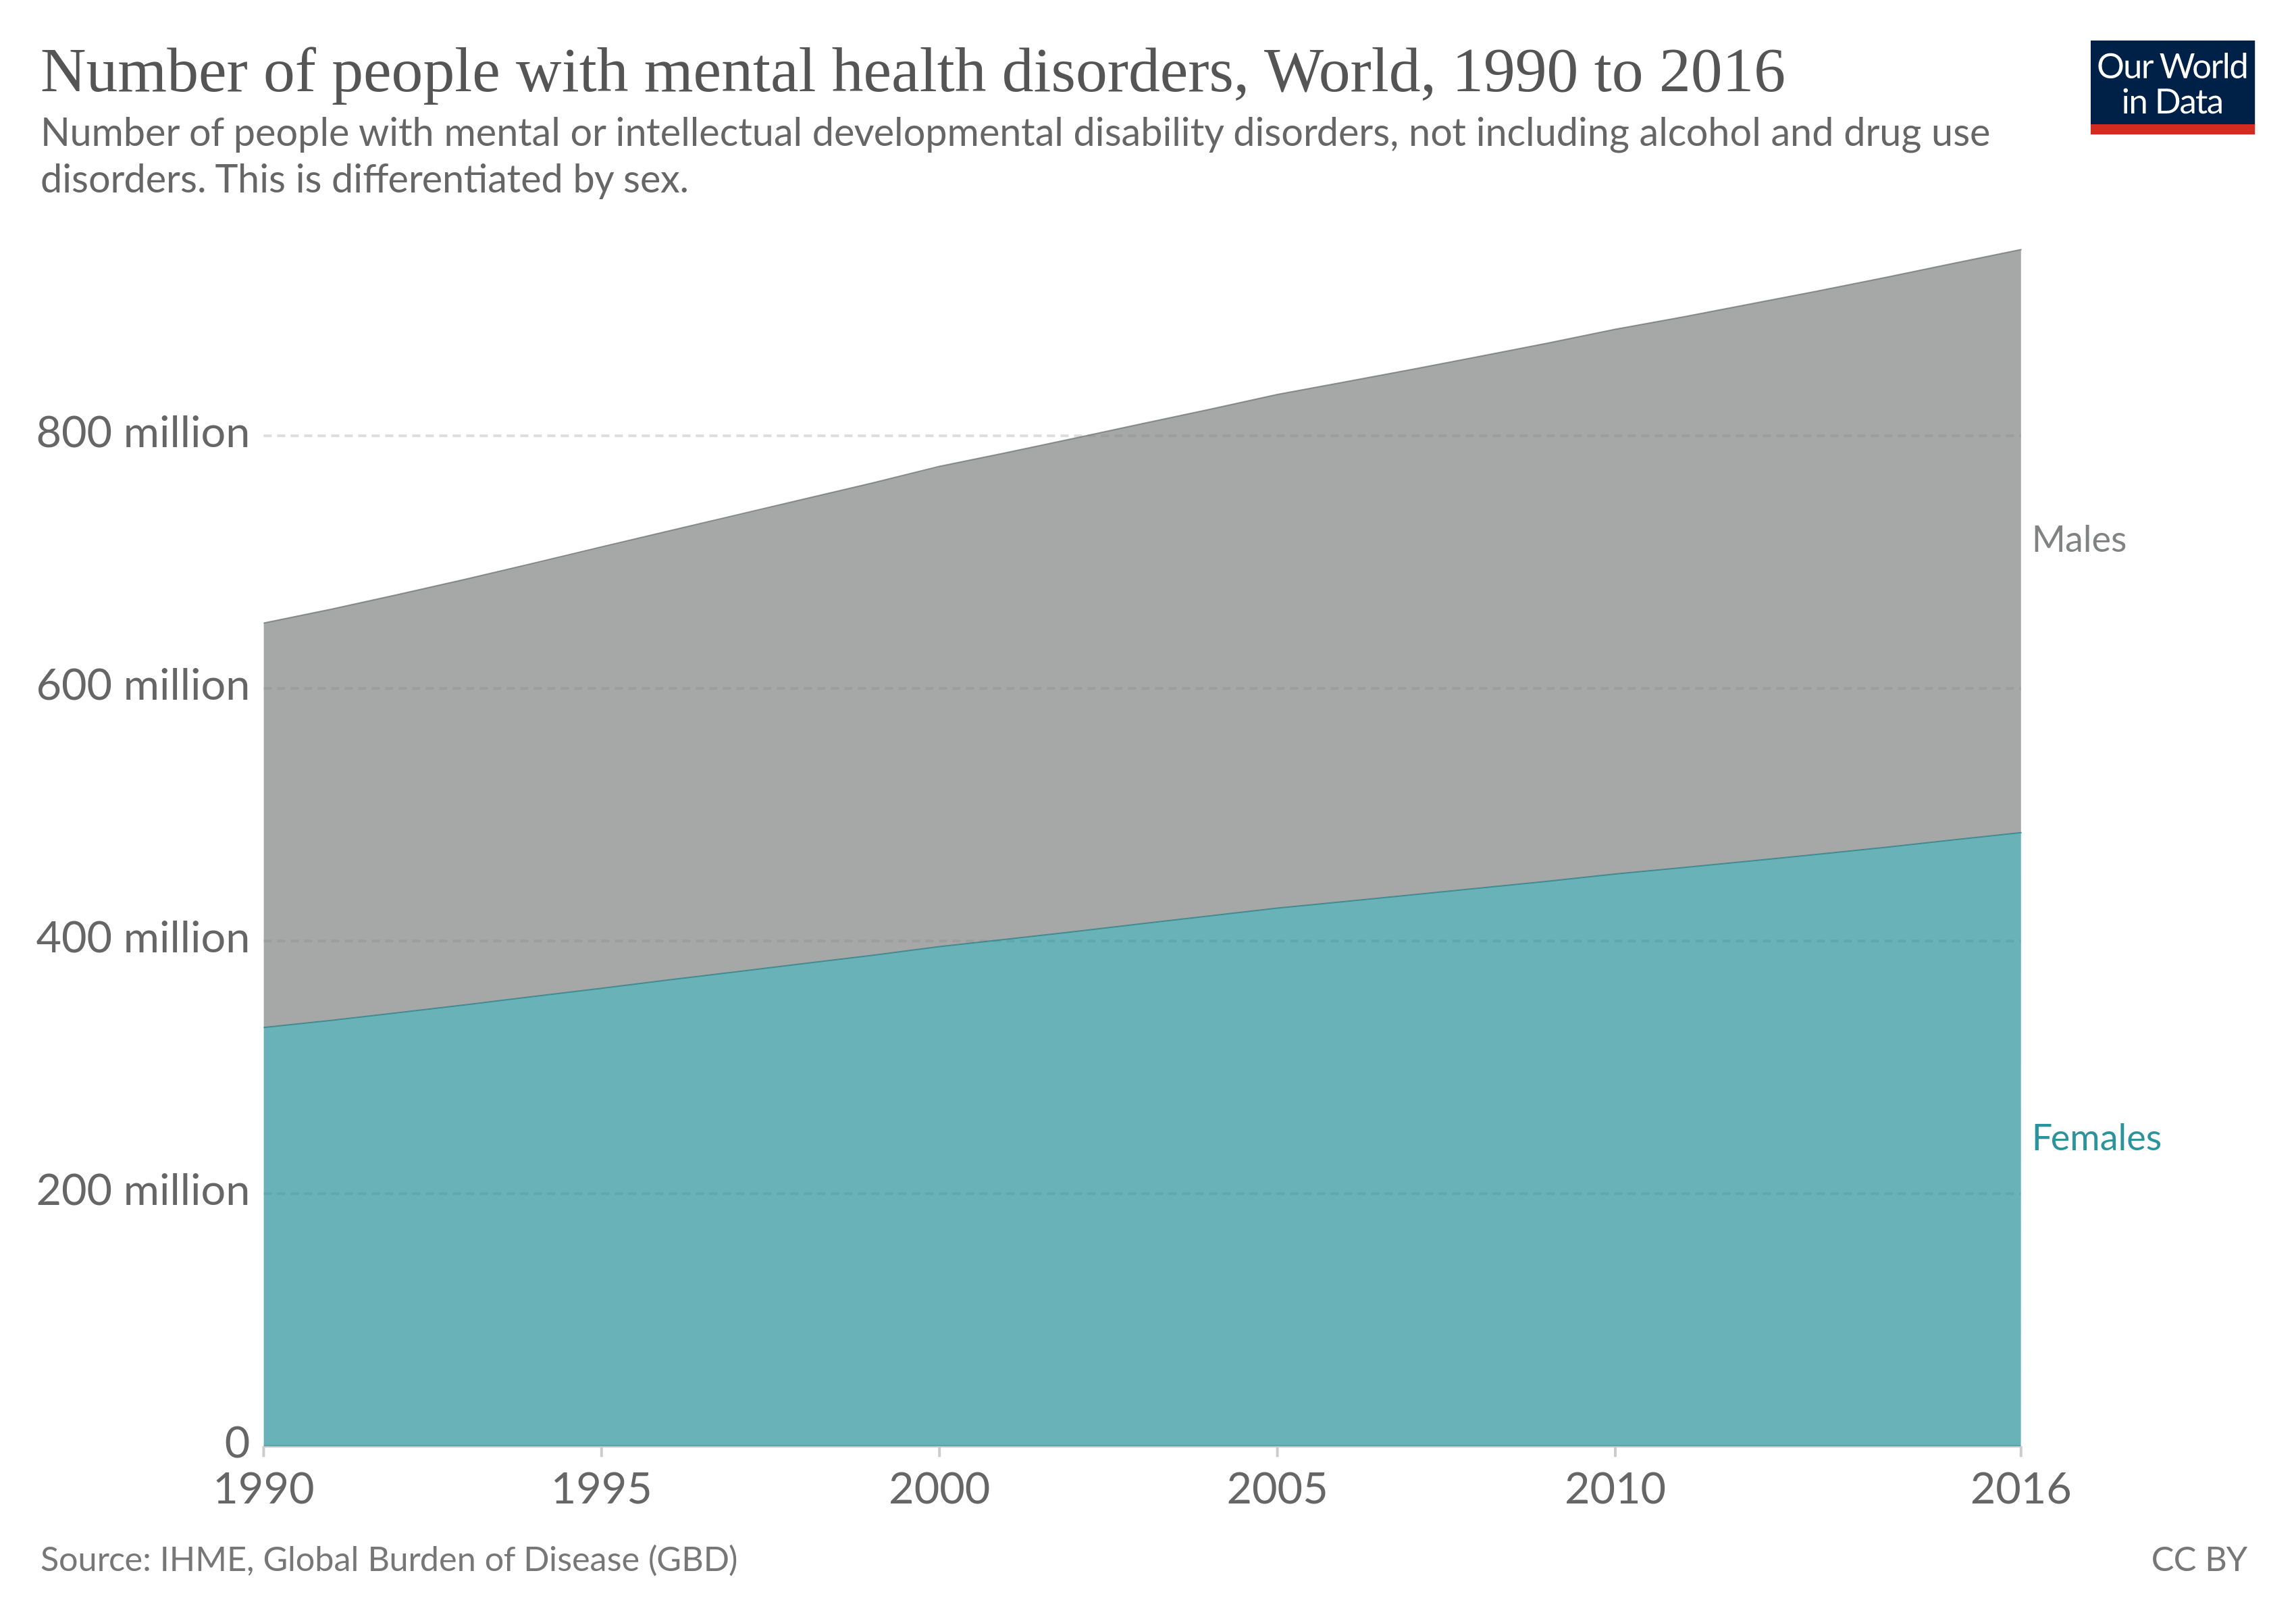
\includegraphics[width=0.75\textwidth]{number_mental_health.png}
  \caption{Number of people with mental health disorders}{Reprinted from \cite{owidmentalhealth}.}
\end{figure}


\subsection{Motivation}

Nowadays, technology is becoming increasingly integrated into our lives. Specifically, smartphones have became a daily basis used tool. People read the news, check the weather, chat with their relatives and friends, etc., using smartphones. Modern chat applications (such as \cite{Telegram}) allow people to create bots that can interact with them like if there was a person on the other side. These chatbots are growingly becoming popular amongst people because they cover many functionalities, from tracking shipments to playing games and reminding tasks. Telegram bots do not require another app to be installed in the client's phone, so the client can save storage space. Chatbots can evolve into conversational-agents-as-sensors are systems that consist on virtual agents that interact with users to retrieve their status in an ubiquitous, continuous, customizable and implicit or explicit way.

As we previously discussed, mental disorders are taboo, so having a bot you could talk with about how your day went, feelings, etc., could lead to an easier way of diagnosing them because chat conversations are seen as ''natural'' by society. The conversational agent will ask the patient a batch of questions (previously defined by their doctor) and show the data to the specialist so that the diagnosis can be more precise.

In addition, the mental specialist-patients ratio is quite low in Spain, about 2 psychologists per 100.000 citizens, \cite{elmundo}. In the future, this lack of specialist will be even more evident, as more people will suffer from mental health disorders. In fact, by 2030 there will be approximately 2 million more adults in the UK with a mental health problem. \cite{nhs}.

\subsection{Objectives}
\label{sec:objectives}
\begin{itemize}
  \item \textbf{Main goal}: to develop a conversational-agent-as-a-sensor which will be able to interact with a person with a disorder and ask questions defined by specialists.
  \item \textbf{Secondary goals}:
    \begin{itemize}
      \item To design a graphical web interface where doctors can consult their patient's responses.
      \item To design a flexible and scalable architecture to add functionality to the system.
      \item To design an architecture based on containers to host the different system modules.
      \item To implement a system that covers the previous goals.
      \item To test a beta version of the assistant in real people and analyse the retrieved data as well as target audience's feelings about it.
    \end{itemize}
\end{itemize}

\subsection{Structure}

The first chapter of this project offers an introduction to the context in which the main goal is intended to be developed as well as an analysis of related papers. This section is divided into four main categories (health application domains, conversational agents types, communication format and architecture) and a research about the popularity of chatbots.

The second one (\textbf{Methodology}) contains the proper requisites design, architecture, programming language and frameworks that are intended to be used in the system development, as well as its the most important modules and some code snippets to illustrate its functionality. The third one (\textbf{Environment Setup}) explains how to deploy both a development and a production environment for HOW-R-U. The fourth chapter (\textbf{Discussion}) analyses the system by performing a SWOT analysis. Finally, the last one (\textbf{Conclusions}) analyses the initial objectives of the project and if they were achieved or not, as well as possible future work.


\newpage

\section{State of the art}

\subsection{Number of publications related to chatbots}

Several queries were performed on \textit{scopus.com} to check the number of articles per year related to chatbots and their applications in health. The results obtained were the following ones:

\begin{figure}[H]
  \begin{subfigure}[t]{0.3\textwidth}
    \centering
    \begin{tikzpicture}
      \begin{axis}[title=\shortstack{chatbot OR "conversational agent"}, ytick distance={100}]
        \addplot table {data/chatbot_or_ca_query_results.dat};
      \end{axis}
    \end{tikzpicture}
  \end{subfigure}
  \hspace{3cm}
  \begin{subfigure}[t]{0.3\textwidth}
    \centering
    \begin{tikzpicture}
      \begin{axis}[title=\footnotesize{\shortstack{(chatbot OR "conversational agent")\\AND\\(coach OR counselor OR assistant)}},
                   ytick distance={15}]
        \addplot table {data/chatbot_or_ca_and_coach_or_counselor_or_assistant_query_results.dat};
      \end{axis}
    \end{tikzpicture}
  \end{subfigure}

  \vspace{0.5cm}

  \begin{subfigure}{\linewidth}
    \centering
    \begin{tikzpicture}
      \begin{axis}[title=\footnotesize{\shortstack{(chatbot OR "conversational agent")\\AND\\(coach OR counselor OR assistant)\\AND\\health}}, ytick distance={5}]
        \addplot table {data/chatbot_or_ca_and_coach_or_counselor_or_assistant_and_health_query_results.dat};
      \end{axis}
    \end{tikzpicture}
  \end{subfigure}
  \caption{Search results of different queries performed in \textit{scopus.com}.}
\end{figure}

We can observe that, in the last 5 years, all of them show a considerable increasing number of articles and papers related to virtual assistants.


\subsection{Health application domains}

Chatbots can be applied to many health domains. For example, \cite{Alesanco2017185} proposes an agent that provides help to perform dermatological medicament prescriptions. \cite{BennetPraba20193470} takes care about nutrition by proposing a chatbot to motivate patients to maintain weight. Another example of conversational interface oriented to health is \cite{Falala-Sechet2019236}. This paper shows a virtual agent that can establish a dialogue with patients to help them go through difficult situations that can affect their psychological status.\\

Chat agents can not only be classified according to the area they area applied to, but also according to the target group. We can find chatbots to help students learn, such as \cite{Lopez2008194} proposal, that offers a simulation of a real patient that presents several symptoms so that students have to interview them and make a diagnostic as a doctor would make in real life. Other interesting project is \cite{Shorey2019e14658}, that intends to improve communication between patients and hospital workers by by creating simulated clinical scenarios with virtual patients so that undergraduates can practise with close to real situations instead of purely theoretical ones.\\

There are also chatbots aimed to help doctors do their work. For example, \cite{Ni201738} offers an agent that interviews sick people before the doctor does. Mandy elaborates a diagnostic based on several questions about patients' symptoms and sends it to the doctor so that can save time. As professional treatments do not last as much, complements such as \cite{DAlfonso2017} are used. They offer a long-term treatment after the professional one so that the patient's progress is not lost. \\

Virtual agents can be also aimed to help patients. For example, \cite{Harilal2020349} is a counsellor that helps patients with depression by establishing empathetic conversations with them. \cite{Roca2020954} suggests an agent that offers help to people by reminding the intake of their medication, sending notifications to caregivers, providing summaries, etc.,

Health coaches can be really helpful. For example, \cite{Breso2016297} proposes a platform to identify and provide early intervention for symptoms of depression and suicide, with a usability of 75.7\% and an accuracy of 70.9\%. Another example is \cite{Hirano2017}, which offers preventive therapy for mental healthcare. The audience's mental health punctuation significantly improved after using the application. Moreover, the usage rate and the number of suggested actions carried out was high. That indicates that people found the app useful. By last, \cite{Ring2016} suggests an agent that responds to users' affective states during virtual therapy sessions. Facial expressions and voices are measured during the session and 70\% of users affirmed that they felt understood by the agent. 50\% of them stated that the agent evoked emotional responses in them during the interactions.

\newpage
\subsection{Conversational agents types and communication formats}

Virtual assistants can be classified attending to their main goal. Coaches help the user to get what he wants. For example, \cite{HUDLICKA2013160} presents a coach that assists people by motivating them to meditate. The paper results showed that using the agent was more effective in helping users to establish a regular meditation habit. \cite{Guo2020} offers another coach that asseses users in their workouts to improve their postural hygiene by using wearables as sensors. Conversational agents can also be counselors, which help the user to identify and solve problems. The research carried out by \cite{Drislane2020158} proves that counselors can be really helpful when trying to reduce alcohol and drugs consumption amongst users. \cite{Yasavur2014381} suggests a virtual therapist that gives brief speech interventions (3-5 minutes) aimed to let a person's alcohol consumption up and make him or her be aware of the problem. \\

They can use different methods to communicate with their audience: text, voice or both. If we focus on speech-enabled conversational agents, we can distinguish \cite{Maharjan2019929}, which proposes a smart speaker that regularly asks its audience about their sleep quality, mood and physical activity. By analysing the given responses and their tone, volume and  intonation the agent is able to extract useful information useful for detecting markers of a possible mental ilness. In text-based chatbots, the user's input can be free (the agent will translate it to an ontology to understand it) or limited (a custom keyboard with fixed options will be shown or the agent will ask the user to enter a valid option). Finally, the most popular virtual assistants are multimodal (they both admit text and speech communication).

\begin{figure}[H]
  \centering
  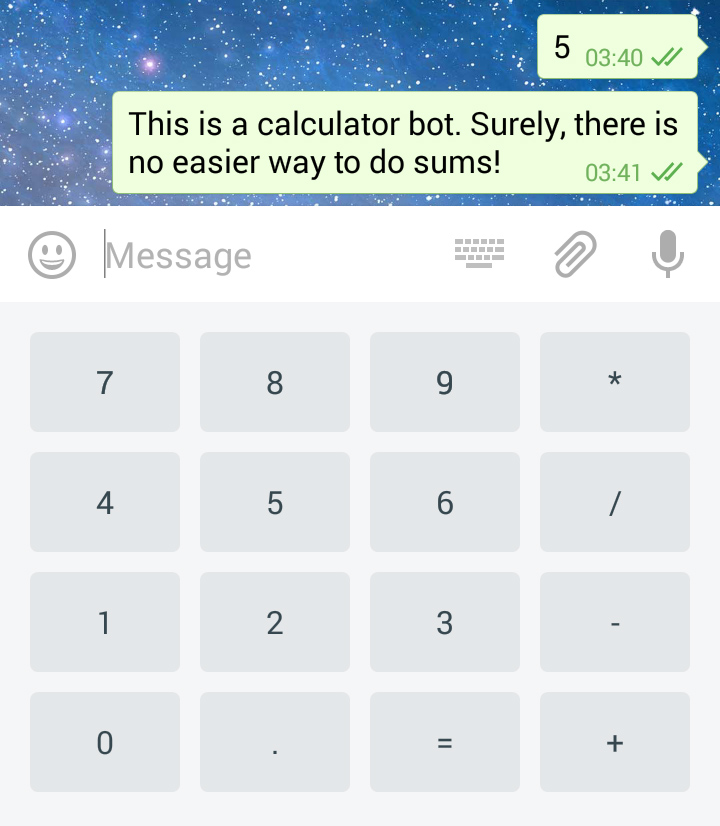
\includegraphics[width=0.5\textwidth]{custom_keyboard.jpg}
  \caption{Example of a custom keyboard for a conversational agent}{Reprinted from https://core.telegram.org/bots.}
\end{figure}


For a more extensive review of the state of the art in this area the reader is directed to \cite{Montenegro201956}.
\newpage
\subsection{Technology}

The chatbot market consists on a variety of chat applications, mainly aimed to smartphone users. However, the wide majority of them count with a web interface or a desktop application so they can be also used on personal computers. After performing some research over the most famous chat applications that allow building conversational agents, the following table was elaborated:

\begin{table}[h!]
  \centering
  \begin{tabular}{|c|c|c|c|}
    \hline
    \textbf{Platform} & \addstackgap{\textbf{\shortstack{Number of daily \\ active users}}} & \textbf{Free API to implement chatbots}  \\
    \hline
    \cite{FacebookMessenger} & 1.66 billion &  \greentick  \\
    \hline
    \cite{Whatsapp} & 1.5 billion & \redcross \\
    \hline
    \cite{WeChat} & 1.083 billion & \greentick  \\
    \hline
    \cite{Telegram} & 0.2 billion & \greentick \\
    \hline
    \cite{Kik} & 0.015 billion & \greentick \\
    \hline
    \cite{Discord} & 0.014 billion & \greentick \\
    \hline
    \cite{Slack} & 0.012 billion &  \greentick \\
    \hline
    \cite{Viber} & 0.008 billion &  \greentick \\
    \hline
    \cite{Line} & 0.00723 billion & \greentick  \\
    \hline
  \end{tabular}
  \caption{Comparison between different chat applications (2019).}
\end{table}


We can see that Whatsapp, which is the most used messaging app, has no free API to develop conversational agents (the one it has is oriented to business). As opposed, the rest of the widely used chat applications offer an API for programmers to build chatbots in an easy way. \\

A key aspect on social networks is the privacy they ensure. \cite{Kosinski5802} shows that Facbook's likes can be helpful to predict people's sensitive attributes such as age, gender or happiness. \cite{Rastogi17} affirms that Whatsapp's end-to-end encryption methods are not secure enough as metadata can reveal private information. On the other hand, \cite{Sutikno16} states that Telegram provides more privacy protection than other apps. One of its main features is that users can create and customize an username so that they do not have to exchange phone numbers to chat (such as in Whatsapp).


\newpage

\section{Methodology}

\subsection{Design}

\subsubsection{Requirements}
The MoSCoW prioritization method \cite{moscow} will be used to classify the requirements of this project. MoSCoW is an acronym for ''\textbf{M}ust have, \textbf{S}hould have, \textbf{C}ould have and \textbf{W}on't have'', categories in which requirements are divided.
\begin{itemize}
  \item \emph{Must have} requirements. They are critical to the success of the project.
    \begin{itemize}
      \item The conversational agent must ask questions defined by doctors to the patients.
      \item The conversational agent must show a custom keyboard to the patient with the possible answers to the questions.
      \item The application must allow doctors and patients enrollment and account deletion.
      \item The application must allow the doctors to download a file with their patients answers between two given dates.
      \item The system must support modularity.
    \end{itemize}
  \item \emph{Should have} requirements. These are important requirements, but not necessary for  the system release.
    \begin{itemize}
      \item The system should be under a CC BY-NC-SA 4.0 \cite{CC} license.
      \item The application should allow the doctors to add, modify and delete questions and their respective answers.
      \item The application should allow the doctors to create public questions so that other doctors can assign them to their patients.
      \item The conversational agent should be able to ask questions following a configurable schedule.
      \item The application should show interactive charts to doctors with their patients data.
     \end{itemize}
  \item \emph{Could have} requirements. Desirable requirements that could improve user's experience or satisfaction. Will be included if there is time at the end of the development.
    \begin{itemize}
      \item The system could implement a numeric priority to manage the order in which questions are asked.
      \item The system could allow the doctors to configure the frequency of each question (only once, daily, weekly, monthly, etc.,).
      \item The system could be translated to other languages.
      \item The application could support password change functionality for doctors.
      \item The application could support two factor authentication for doctors.
      \item The conversational agent could support groups.
      \item The system could allow doctors and patients to delete all their data from the system.
      \item The agent could offer an option to the patients to view and modify their profile data.
      \item The applications could allow doctors to assign a question to all their patients when creating it.
      \item The system could support more timezones.
    \end{itemize}
  \item \emph{Won't have} requirements. They are inappropiate or the least important ones, so they are not included in the project.
    \begin{itemize}
      \item The application won't be cross-platform.
      \item The system won't share the retrieved data with third parties.
    \end{itemize}
\end{itemize}
\newpage
\subsubsection{Architecture}

The requirements that have been listed in the previous section are summarized in the following architecture:
\begin{figure}[H]
    \makebox[\linewidth]{
        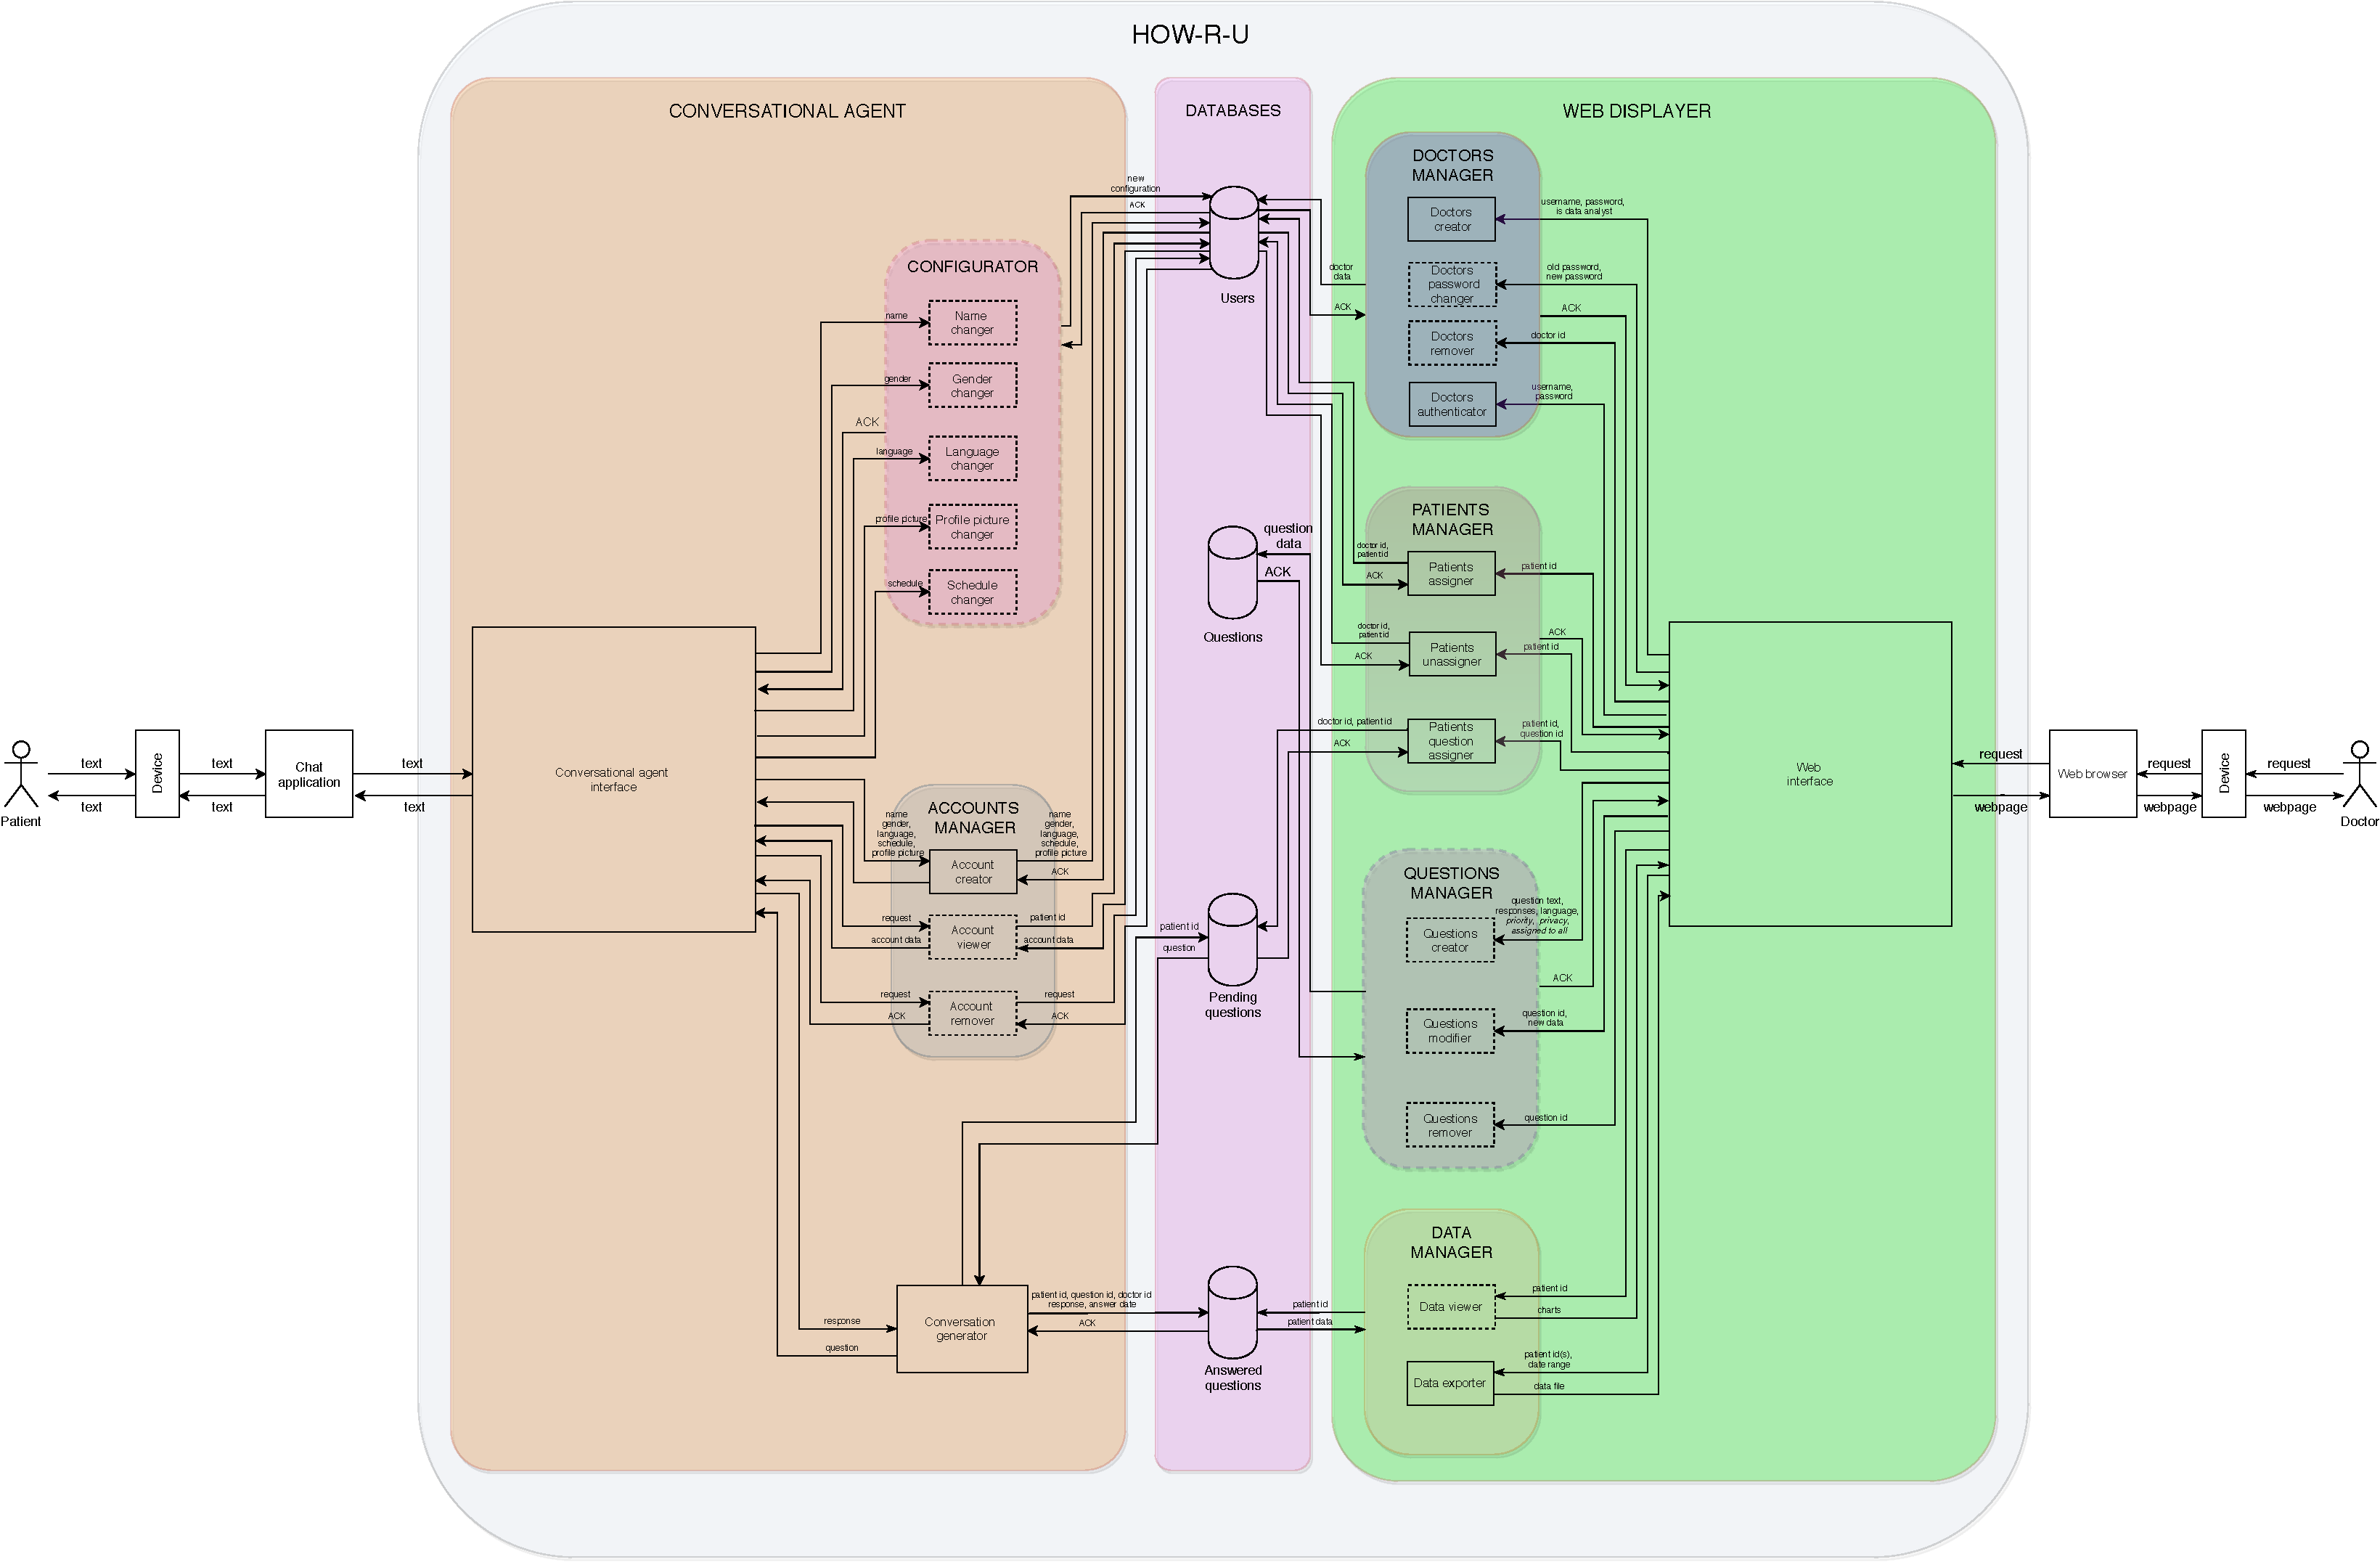
\includegraphics[width=1.35\linewidth, angle=-270]{architecture.pdf}
    }
    \caption{System architecture. Created using \emph{diagrams.net} \protect\cite{drawio}.}
\end{figure}

\begin{figure}[H]
    \makebox[\linewidth]{
        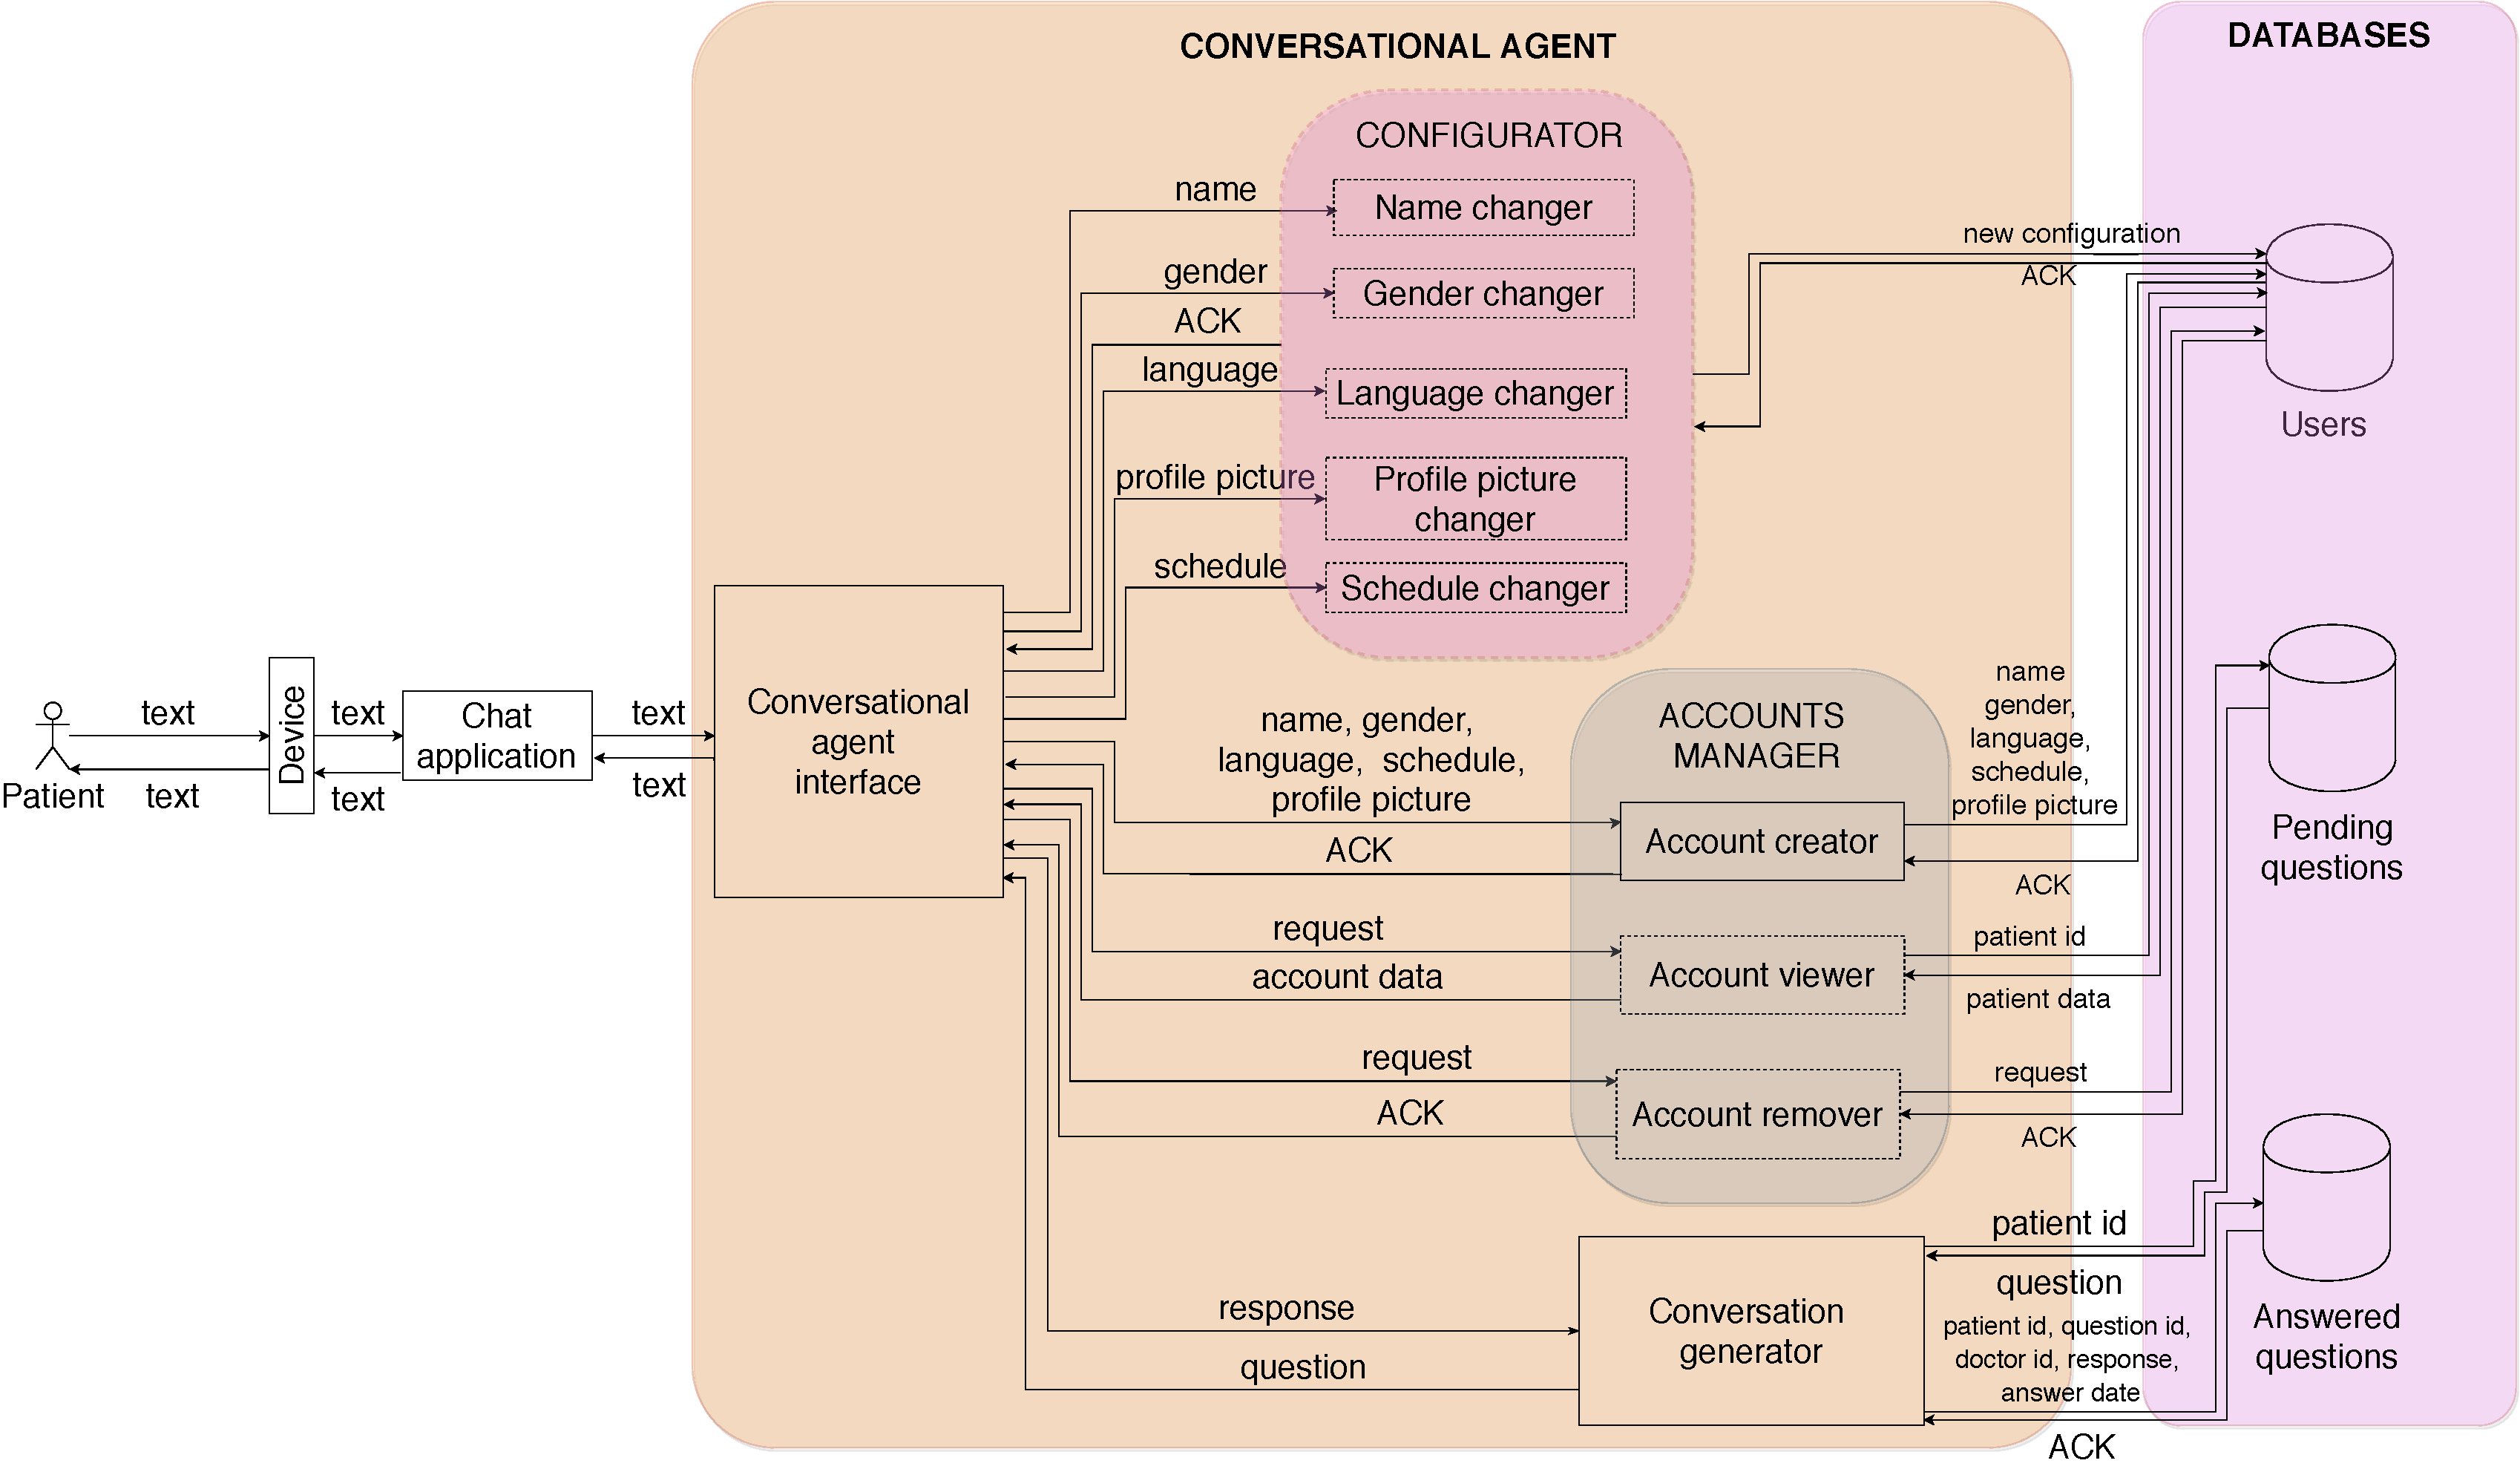
\includegraphics[width=0.95\linewidth]{conv_agent.pdf}
    }
    \caption{System architecture (conversational agent and databases).}
\end{figure}

\begin{figure}[H]
    \makebox[\linewidth]{
        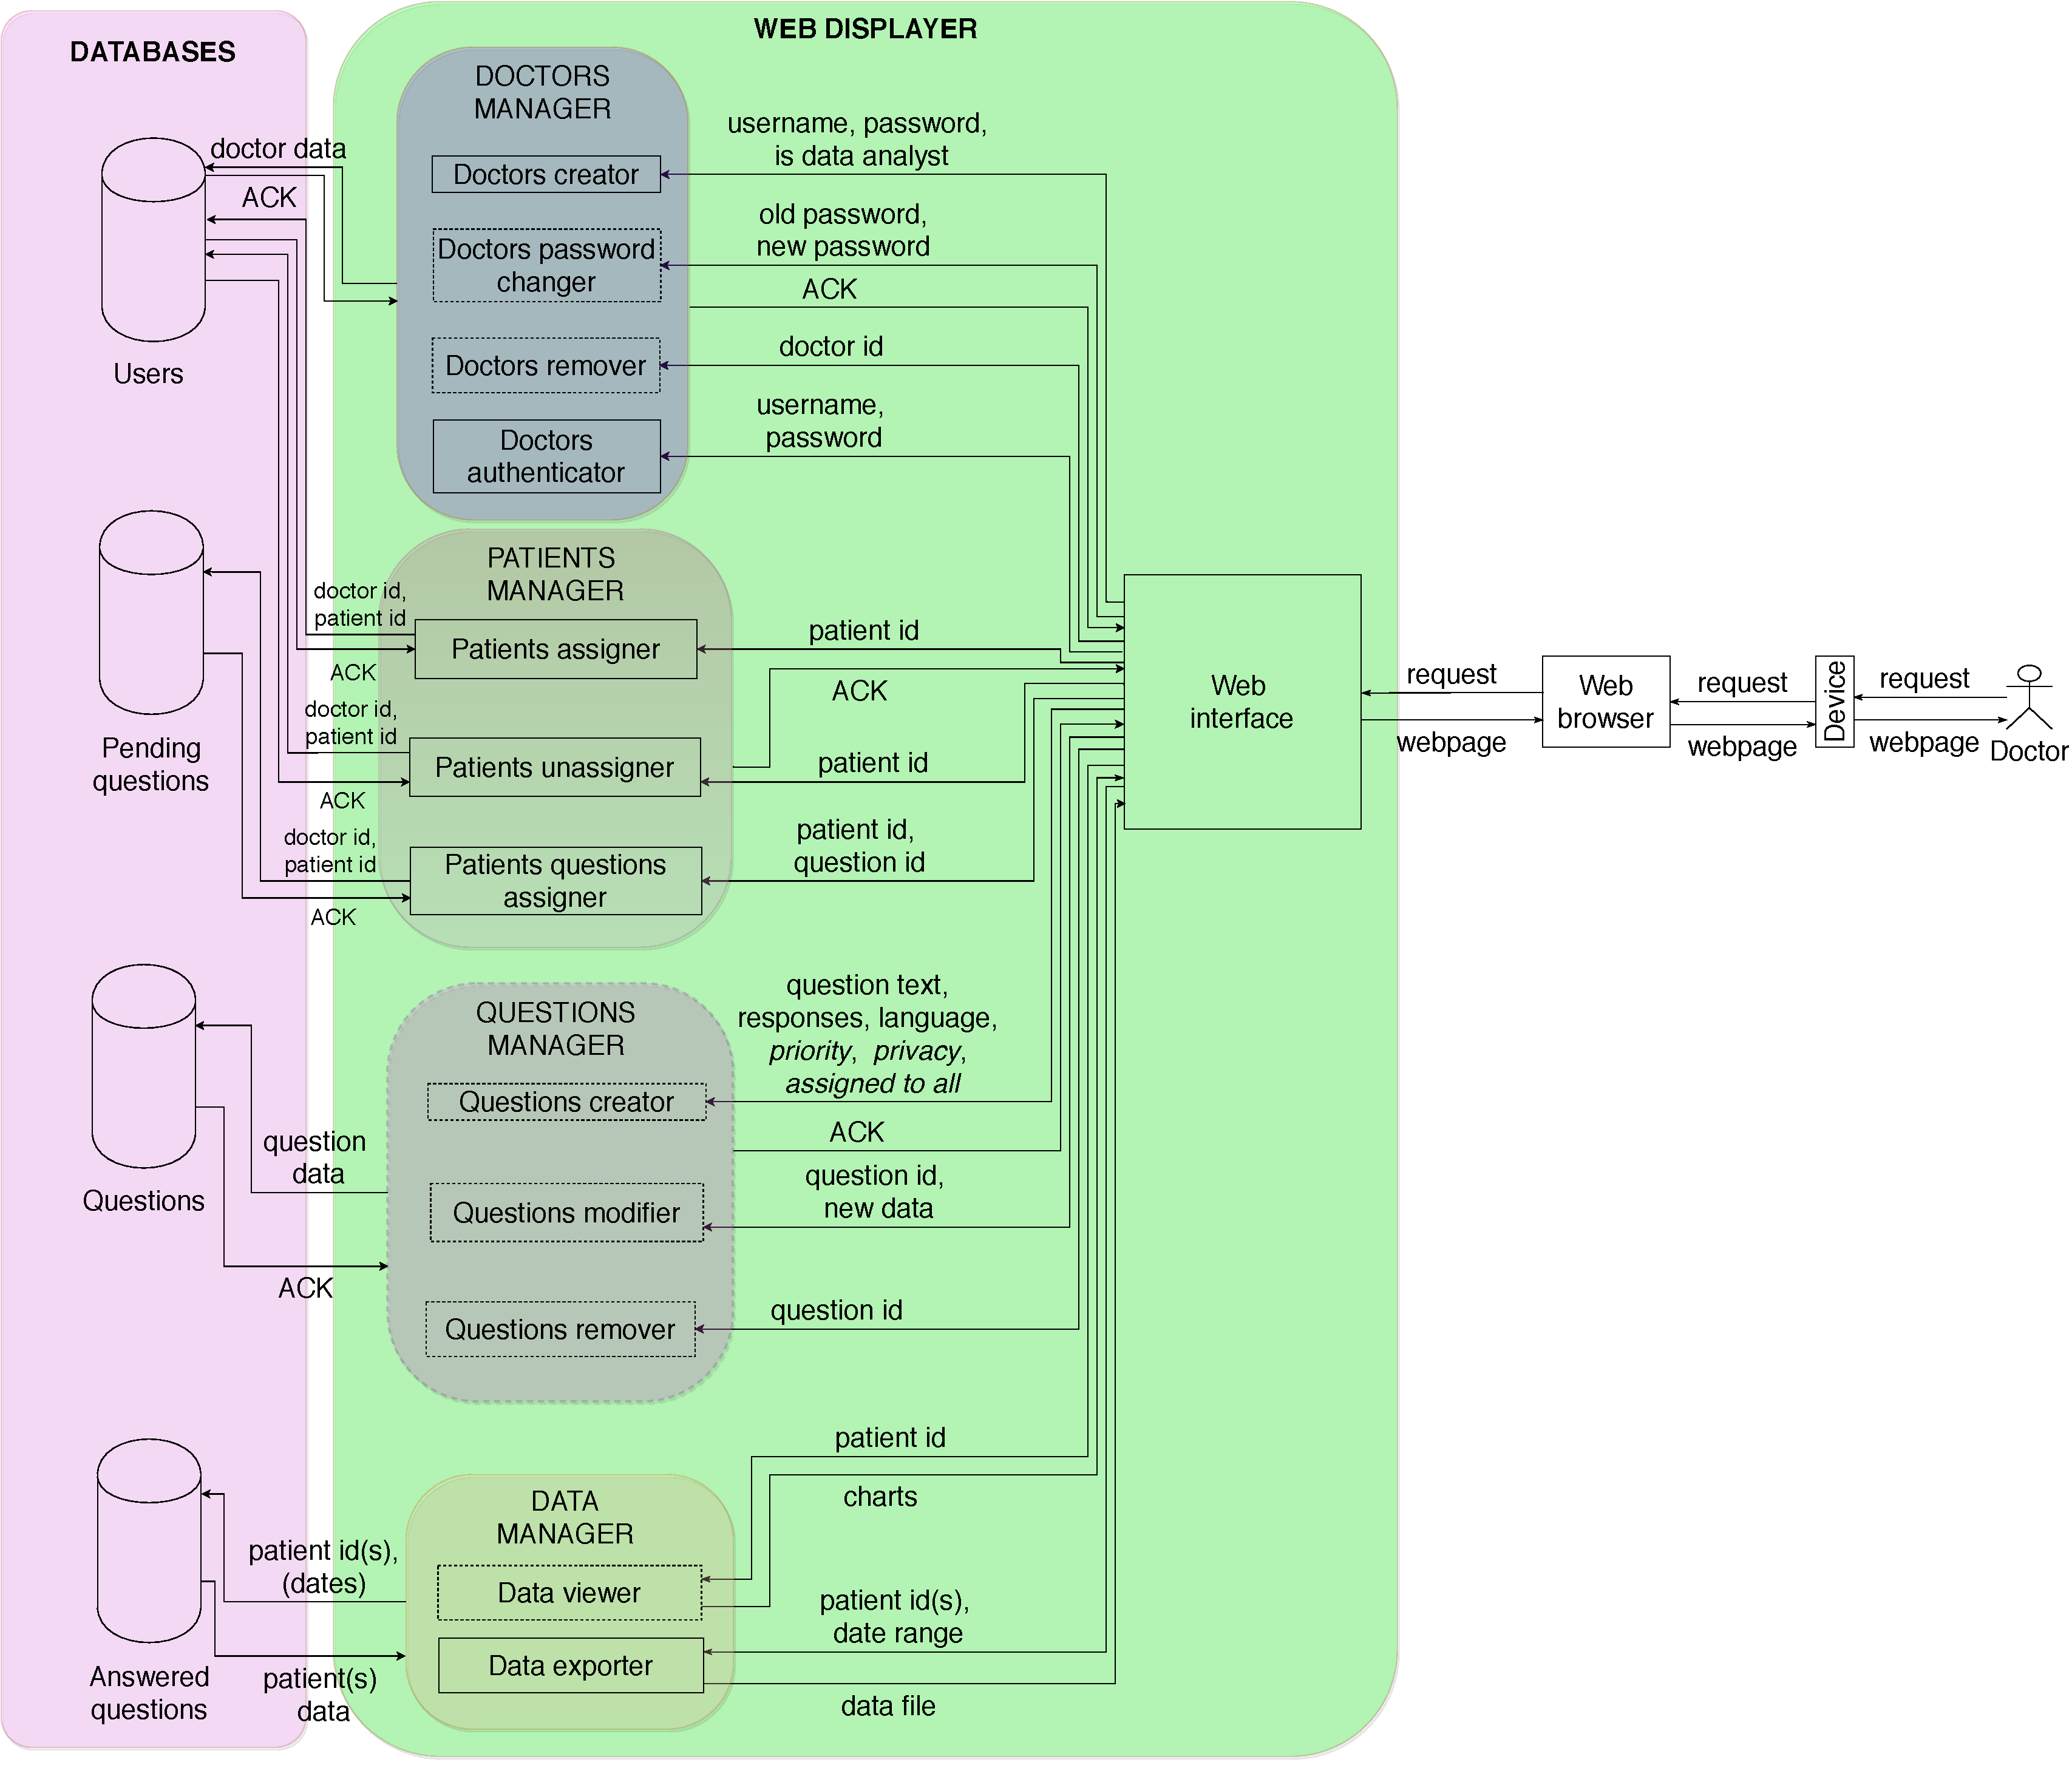
\includegraphics[width=0.98\linewidth]{web_int.pdf}
    }
    \caption{System architecture (web interface agent and databases).}
\end{figure}


Italic text and dashed lines represent optional features (should and could requirements), whereas continuous  lines refer to mandatory ones (must). The architecture is divided into three main modules: conversational agent, databases and web interface. The conversational agent is in charge of interacting with patients by asking them questions, allowing them to change their settings, etc., On the other hand, the web interface provides the corresponding information for doctors (retrieves answers, associated patients, etc.,) as well as lets them create new questions, associate patients, etc., Finally, the databases store the corresponding data.

HOW-R-U is structured in four main databases. The users database contains doctors and patients information and their corresponding configurations. Patient objects stored in this database have properties such as name, username, chat id, gender, language, schedule and profile picture, whereas Doctor entries contain attributes like username, password, wether the doctor is a data analyst and session information. Questions database contain Question entries, consisting on question text, possible responses, question language, priority, frequency and author. Pending questions database holds entries that link a doctor, a question and a patient. Moreover, they also include a flag that determines if the question (assigned by the corresponding doctor) is being answered right now by the related patient. Finally, Answered questions database contains entries that also link a patient, a doctor and a question. They include two more properties: response given by the patient and answer date.

The conversational agent is formed by three submodules, triggered by different events. The first one is the accounts manager, including three components. The first one is the Account Creator, in which the conversational agent will ask the user the language in which the interface will be shown, their name, gender, profile picture and schedule for questions. This event is triggered when the patient interacts with the agent for the first time. The second one is the Account Viewer, which shows the patient all the details about their account. Finally, the Account Remover allows the patient to completely delete all their data from the system in an unrecoverable way. These two last components are triggered by an specific command sent by the patient.

The second module is the configurator. It is also triggered by a command. This interface shows a menu with the available options: change name, gender, language, profile picture or schedule. All these actions have a fallback command to cancel the current operation. When an operation is completed, the corresponding data is retrieved, modified or deleted from the Users database.

Finally, the last module is the Conversation Generator, that is triggered when the schedule time comes. The system will check the pending questions database to check if the user has to answer at least a question today. If the previous condition is fullfilled, the question will be prompted, along with a custom keyboard showing the different answers. Everytime a question is answered, an AnsweredQuestion entry containing the patient id, question id, doctor id and answer date is created and stored in the corresponding database. When all the pending questions have been answered, this flow terminates and the agent thanks the user. If there are no questions to ask, the chatbot will inform the patient.

Last but not least, the web interface interface contains four submodules. The first one is the doctors manager, which permits accounts creation, password change, authentication and deletion. The second one is the patient manager, which lets doctors to assign and unassign patients to its account as well as assign or unassign questions to them. The third one is the questions manager, which allows doctors to create, modify and delete questions. Finally, the data manager offers doctors the possibility to observe charts created with the patient's answers along the time or download a file containing all these data between two dates.




\subsection{Implementation}

The main software that has been used to implement this project is be the following:
\begin{itemize}
  \item Python 3.6.10 \cite{python} as the main programming language for both the web interface and the agent. The following libraries will also be used:
  \begin{itemize}
    \item \emph{python-telegram-bot} to develop the conversational agent.
    \item \emph{ujson} to create and read JSON files in a fast way.
    \item \emph{pytz} for timezone management.
    \item \emph{psycopg2} to connect python with the database management system.
    \item \emph{pillow} to work with images.
  \end{itemize}
  \item Django 3.0.6 \cite{django} as the framework to develop the web interface.
  \item PostgreSQL 12.3 \cite{postgres} as the database management system.
  \item Nginx 1.17 \cite{nginx} as the reverse proxy to redirect the requests from users to the web interface.
  \item Docker 19.03.6 \cite{docker} as the platform where the developing environment is built on.
  \item Telegram \cite{Telegram} as the platform where the conversational agent will offer its services to the patients.
\end{itemize}

HOW-R-U will be structured in the following way:

\begin{figure}[H]
  \centering
    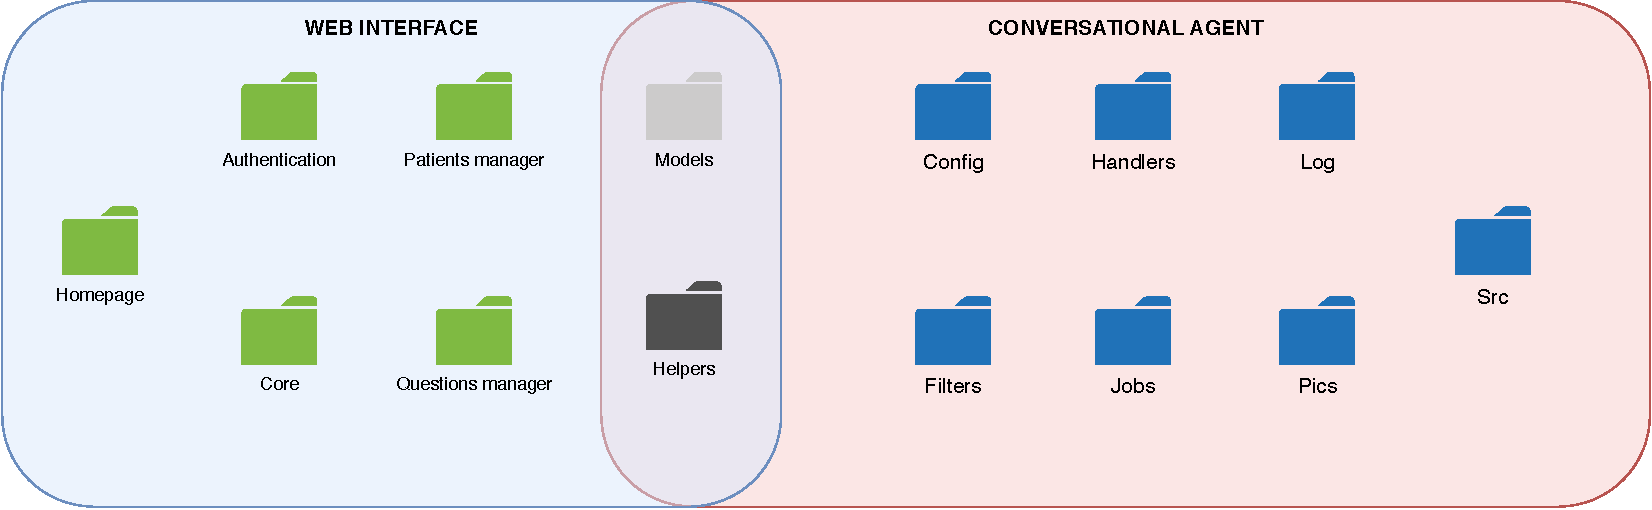
\includegraphics[width=\textwidth]{repo_structure.pdf}
    \caption{HOW-R-U modules structure. Created using \emph{diagrams.net} \protect\cite{drawio}}
\end{figure}

In addition, the system will be prepared to be compatible with Docker in order to deploy a HOW-R-U development environment by including a folder with \emph{Dockerfiles}, \emph{docker-compose} and configuration files.
\newpage
\subsection{Submodules: models and helpers}

Models will be a submodule shared by both the web interface and the conversational agent. It will contain the definition of the different system classes. Django ORM will be used in both of them to simplify database and model operations. To add django to the conversational agent, a custom \emph{manage.py} with the system settings (such as database details and models specification) has been created:

  \begin{python}[caption={Custom \emph{manage.py} file to use Django ORM in the agent. Based in \href{https://stackoverflow.com/questions/45595750/use-django-orm-outside-of-django}{https://stackoverflow.com/questions/45595750/use-django-orm-outside-of-django}}, captionpos=b]
  #!/usr/bin/env python
  import json
  import sys
  import django
  ROUTES_FILE_PATH = '/etc/howru/cfg/routes.json'
  with open(ROUTES_FILE_PATH) as routes_file:
    json_file = json.load(routes_file)
    NAME = json_file['name']
    USER = json_file['user']
    PWD = json_file['password']
    HOST = json_file['host']
    PORT = json_file['port']
  DATABASES = {
    'default': {
        'ENGINE': 'django.db.backends.postgresql',
        'NAME': NAME,
        'USER': USER,
        'PASSWORD': PWD,
        'HOST': HOST,
        'PORT': PORT,
    }
  }

  INSTALLED_APPS = [
    'howru_models',
    'django.contrib.contenttypes',
    'django.contrib.auth'
  ]
  from django.conf import settings
  settings.configure(
    DATABASES=DATABASES,
    INSTALLED_APPS=INSTALLED_APPS,
    USE_TZ=True
  )
  django.setup()
  \end{python}

HOW-R-U models will follow the class diagram below:

\begin{figure}[H]
    \makebox[\linewidth]{
        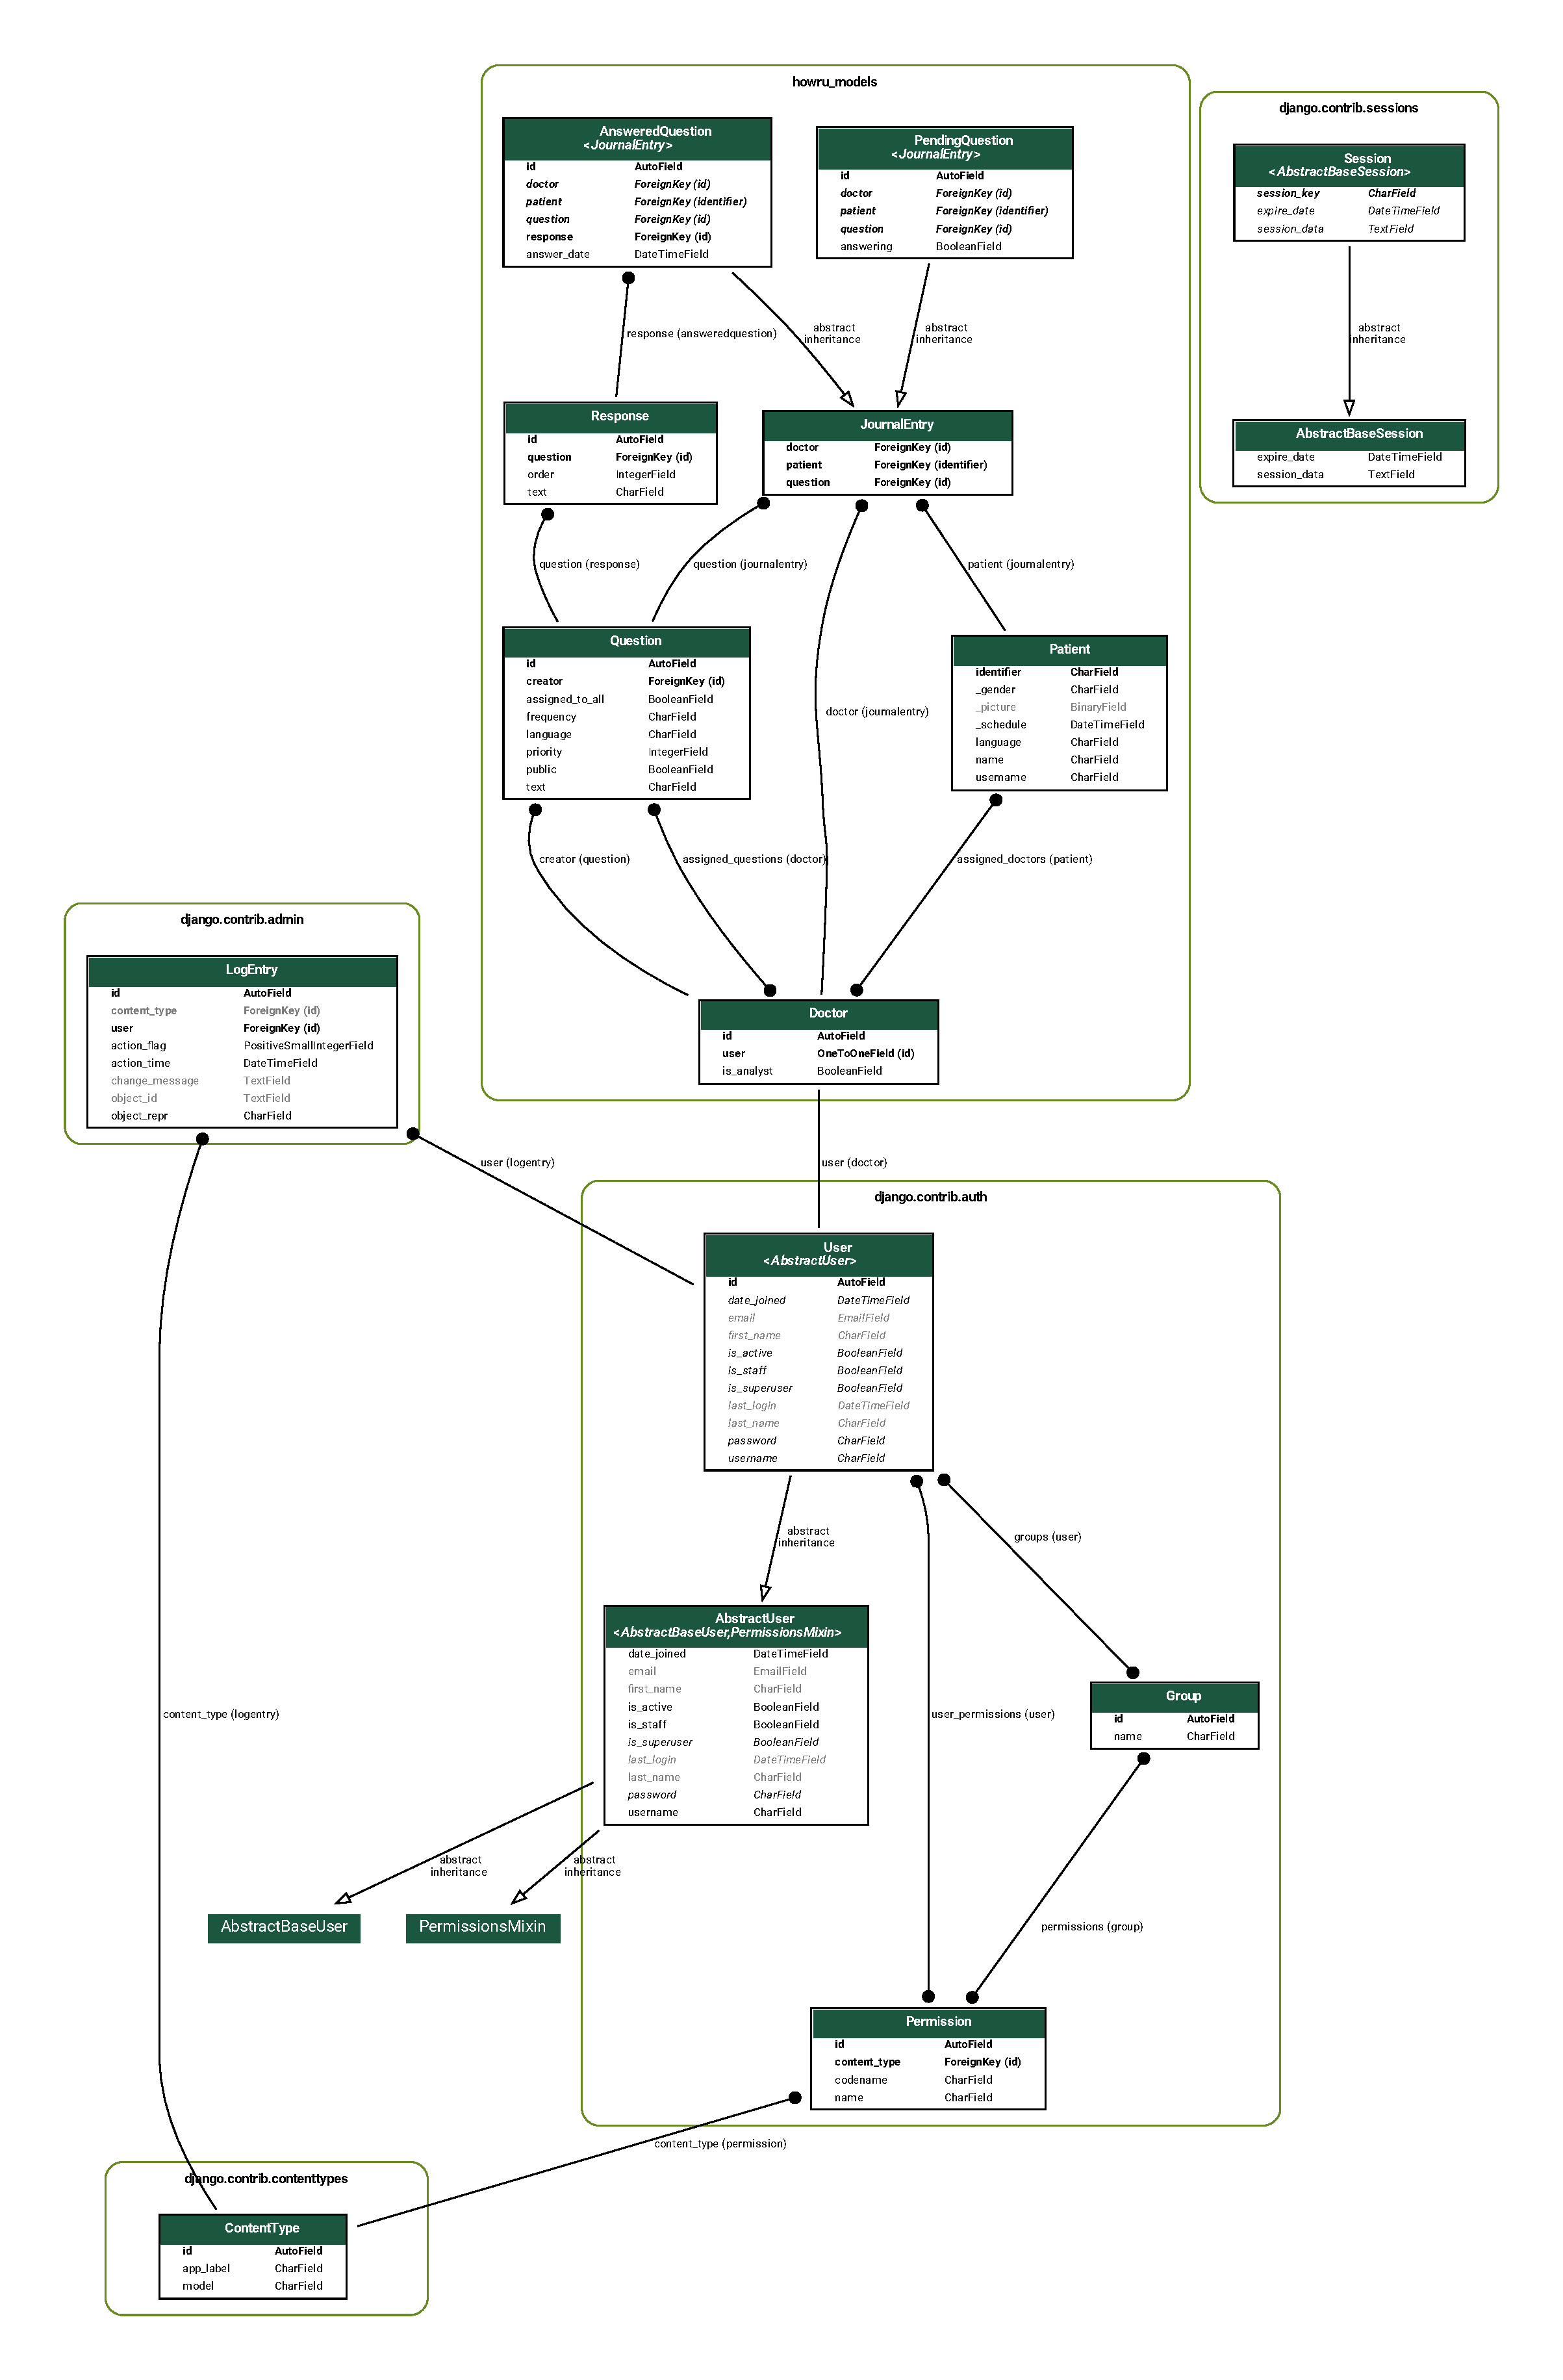
\includegraphics[width=\linewidth]{class_diagram.pdf}
    }
    \caption{System class diagram. Generated by \emph{django-extensions} \protect\cite{django}.}
\end{figure}

\begin{figure}[H]
    \makebox[\linewidth]{
        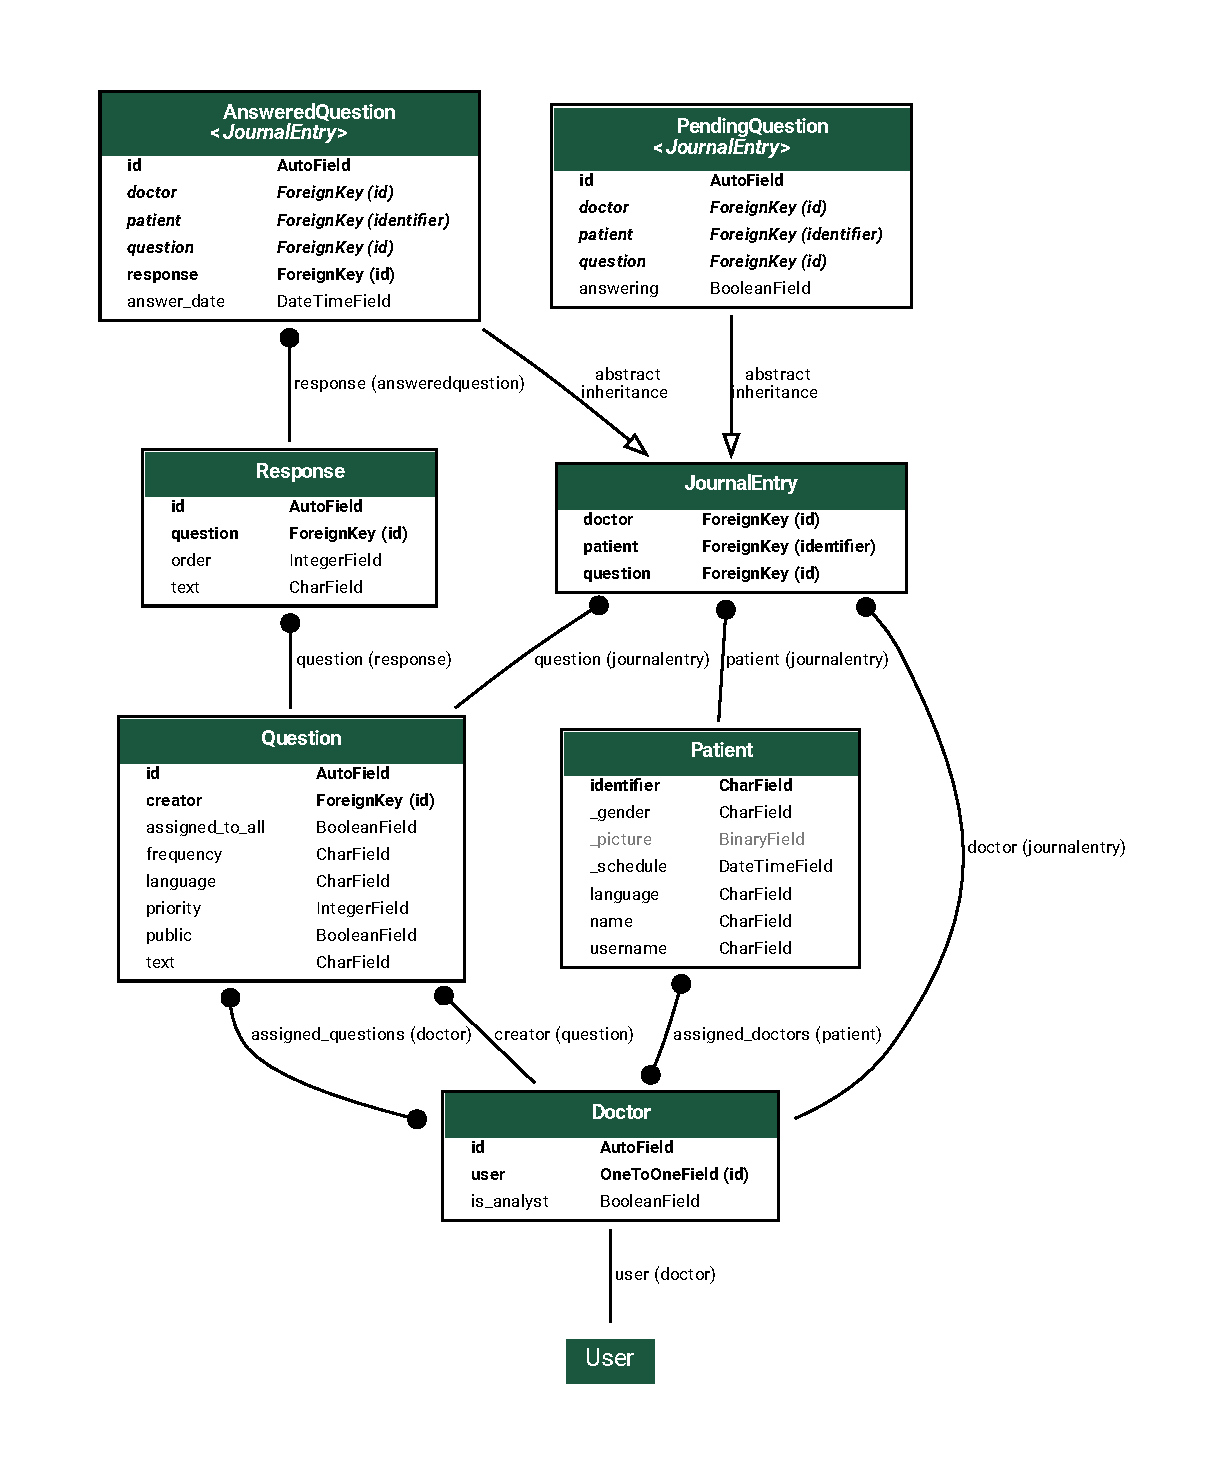
\includegraphics[width=\linewidth]{class_diagram_zoom.pdf}
    }
    \caption{System class diagram (HOW-R-U classes).}
\end{figure}

As we can see, there are six main models in \emph{howru\_models}: Doctor, Patient, Question, Response, Pending Question and Answered Question (both inherit from JournalEntry, an abstract model). A Doctor has a one-to-one relationship with an user, a \emph{Django} pre-defined model which takes care of all authentication, permissions, logs and session logic.

The other submodule, helpers, allows coding and decoding flag emojis from country codes and managing time conversions between UTC (the main time standard in the world) and the timezone in which the system is configured.

\subsection{Conversational agent}


The conversational agent module contains seven submodules: \emph{config}, where the secret token is stored and messages, a file which contains all the messages the bot can send in English and Spanish. The bot secret token is a string which contains an unique identifier that links a Telegram bot user with the code it will run. This token is given by \emph{@BotFather} \cite{botfather}, a bot used to create bots. More information about the bot creation process will be explained in the \hyperref[sec:env_setup]{environment setup section}.

The next submodule, \emph{handlers}, defines the bot behaviour according to certain events, like sending the \emph{/start} command (the first one that is sent when an user interacts with a bot), sending the {\emph{/config}} one, etc., There are three main handlers:
\begin{itemize}
  \item Start handler: asks the patients for their name, gender, language, schedule, and profile picture.
  \item Config handler: manages the configurator module, as well as the account viewer and remover.
  \item Questions handler: handles the questions prompting and answering.
\end{itemize}

Handlers are triggered by a certain event, catched by filters. For example, to catch the \emph{/start} message sent by the patient, the implemented procedure is the following:

\begin{python}[caption={Patient start callback}, captionpos=b]
GENDER, PICTURE, LANGUAGE, SCHEDULE = range(4)
@send_typing_action
def start(update, context):
    """
    Shows welcome message and asks for language
    """
    # Check that user is not registered
    try:
        patient = Patient.objects.get(identifier=update.message.from_user.id)
        logger.info(
            f'User {update.message.from_user.username} tried to register again.')
        update.message.reply_text(text=messages[patient.language]['already_exists'])
        return ConversationHandler.END
    except Patient.DoesNotExist:
        # The user should not exist in DB
        context.user_data['patient'] = Patient(name=update.message.from_user.first_name, identifier=str(update.message.from_user.id), username=update.message.from_user.username)
        logger.info(f'User {update.message.from_user.username} started a new conversation')
        update.message.reply_text(text=f'Hi {update.message.from_user.first_name}. Welcome to HOW-R-U psychologist bot.\nHola {update.message.from_user.first_name}. Bienvenido al bot psicologo HOW-R-U')
        update.message.reply_text(text=f'Please select a language:\nElija un idioma por favor:', reply_markup=keyboards.language_keyboard)
    return LANGUAGE

  <--------------->

  start_handler = ConversationHandler(
      entry_points=[CommandHandler('start', start)],
      states={
          LANGUAGE: [MessageHandler(Filters.regex(f'^({Flag.flag("es")}|{Flag.flag("gb")})$\dollar$'), language)],
          GENDER: [MessageHandler(Filters.regex('^(Male|Female|Other|Masculino|Femenino|Otro)$\dollar$'), gender)],
          PICTURE: [MessageHandler(Filters.photo, picture), CommandHandler('skip', skip_picture)],
          SCHEDULE: [MessageHandler(Filters.regex('^([0-1]?[0-9]|2[0-3]):[0-5][0-9]$\dollar$'), schedule)]
      },
      fallbacks=[],
      name="starter"
  )
\end{python}

We can see how the \textbf{start} command is the entry point of the start handler. When the event is detected, \textbf{start} callback is invoked. This callback ensures that the patient is not already registered (if so, informs the user and finishes the conversation) and prompts a welcome message as well as a custom keyboard with flags, one for each available language. Then, it returns \emph{LANGUAGE}, an state that shows that the agent is waiting for language selection. Start callback creates a Patient object whose data will be filled in the following procedures and stores it in context user data, a reserved storage space for each user. After language, profile picture, gender and schedule are asked, the agent finally saves the entry in the database in the following way:

\begin{python}[caption={Patient saver callback}, captionpos=b]
  @send_typing_action
  def finish(update, context):
      """
      Saves patient in DB, assigns him/her to data_analyst, creates PendingQuestion entries for assigned_to_all questions and finally creates the user's PendingQuestionJob
      """
      patient = context.user_data['patient']
      patient.save()
      # Add patient to data analysts and assigned_to_all questions
      try:
          data_analysts = Doctor.objects.filter(is_analyst=True)
          for doctor in data_analysts:
              patient.assigned_doctors.add(doctor)
              patient.save()
              assigned_to_all = doctor.assigned_questions.filter(assigned_to_all=True)
              for question in assigned_to_all:
                  pending_question = PendingQuestion(doctor=doctor, question=question, patient=patient, answering=False)
                  pending_question.save()
          logger.info("Patient %s assigned to data_analysts", patient.username)
      except:
          logger.exception("Exception while adding patient %s to data_analysts.", patient.username)
      update.message.reply_text(messages[patient.language]['registration_ok'])
      logger.info(f'Creating pending_questions job for user {update.message.from_user.username}')
      PendingQuestionJob(context, patient)
      return ConversationHandler.END
\end{python}

The database entry is created simply with the command \emph{patient.save()} thanks to \emph{django} ORM. After saving the patient for the first time, we need to assign it to all data analysts in the system and assign him/her the questions the analyst have created and configured as assigned to all. Finally, a \emph{job} is created so that assigned questions to the patient are sent. When these procedures are completed, the callback returns \emph{ConversationHandler.END}, indicating that the conversation has ended.

\begin{figure}[H]
  \centering
  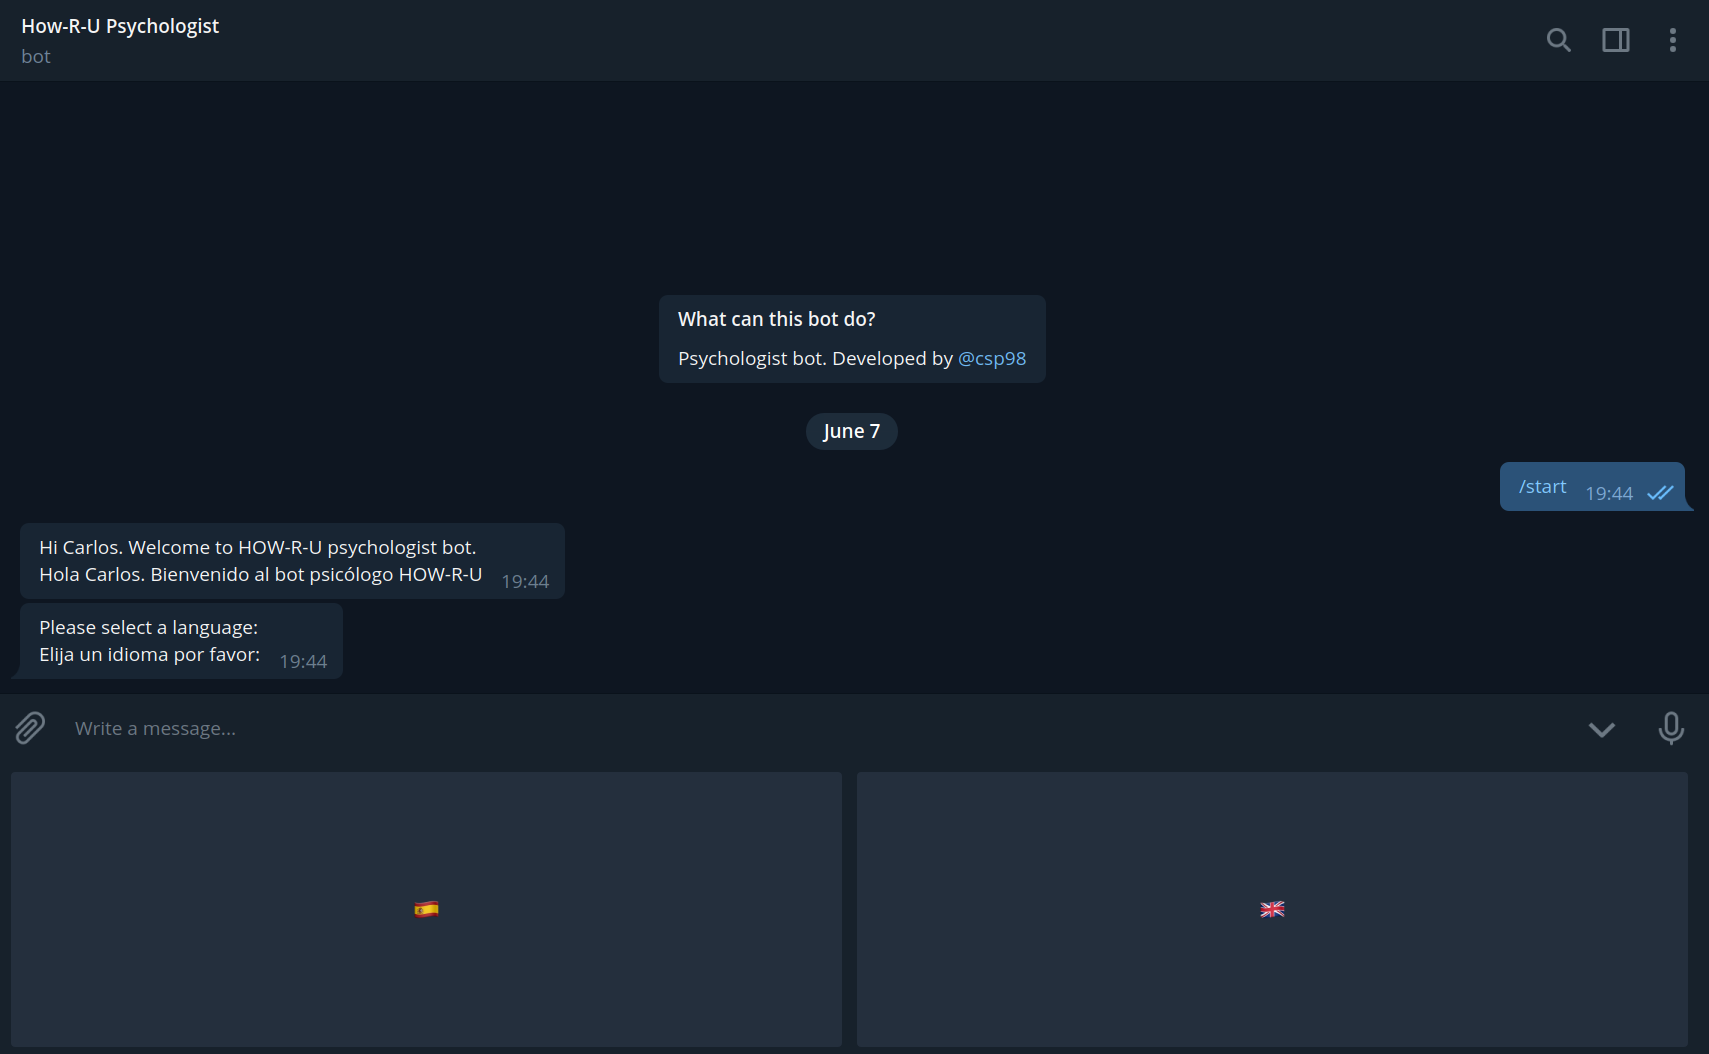
\includegraphics[width=0.45\textwidth]{start.png}
  \caption{Agent showing the welcome message and asking for language selection.}
\end{figure}
\newpage
The \emph{config handler} is invoked when the \emph{/config} command is sent. This command appears in a pop-up menu next to the text input. The configurator callbacks are pretty similar between them. There are two types of them: \emph{ask\_for\_$<$property$>$} and \emph{process\_$<$property$>$}. The first ones send a message to the patients with the old value of the property they want to change and ask them to send the new value. The second ones update the patient's database entry with the new value. For example, the schedule changer is implemented as follows:

\begin{python}[caption={Name changer configurator callbacks}, captionpos=b]
  @send_typing_action
  def ask_change_language(update, context):
      """
      Sends old language to the user and asks for the new one
      """
      patient = context.user_data['patient']
      logger.info(f'User {update.message.from_user.username} asked to change language')
      update.message.reply_text(messages[patient.language]['current_language'] + patient.language)
      update.message.reply_text(messages[patient.language]['change_language'], reply_markup=keyboards.language_keyboard)
      return PROCESS_LANGUAGE

  @send_typing_action
  def process_language(update, context):
      """
      Saves the new language
      """
      patient = context.user_data['patient']
      patient.language = Flag.unflag(update.message.text)
      patient.save(update_fields=['language'])
      logger.info(f'User {update.message.from_user.username} changed language to {patient.language}')
      update.message.reply_text(messages[patient.language]['language_updated'])
      return config_menu(update, context)
  <------------------->
  config_handler = ConversationHandler(
      entry_points=[CommandHandler('config', config)],
      states={
          CHOOSING: [
                     MessageHandler(Filters.regex('^(Cambiar nombre|Change name)$\dollar$'), ask_change_name),
                     MessageHandler(Filters.regex(f'^(Cambiar idioma|Change language)$\dollar$'), ask_change_language),
                     .....
                     ],
          PROCESS_NAME: [MessageHandler(~is_answering_filter & ~Filters.command, process_name)],
          PROCESS_LANGUAGE: [MessageHandler(Filters.regex(f'^({Flag.flag("es")}|{Flag.flag("gb")})$\dollar$'),
                                            process_language)],
          .....
      },
      fallbacks=[CommandHandler('cancel', cancel),
                 CommandHandler('exit', _exit)],
      name="configurator"
  )

\end{python}

The name changer needs a specific filter. As the desired input format is text, we need to distinguish between text and a command (started by \emph{/}). To do so, the command filter is negated (\emph{\~{}Filters.command}). In addition, the agent must distinguish when the name is being changed (a string is expected) and a question is being answered (a string is also being expected). To do so, a custom filter has been developed. This filter matches when a question is being answered at the moment (\emph{~is\_answering\_filter}). Finally, these two filters are combined using an \emph{AND} logic operation. Last but not least, \emph{/cancel} allows the user to cancel the current operation and go back to the configurator menu and \emph{/exit} closes the configurator.

\begin{python}[caption={IsAnswering filter}, captionpos=b]
class IsAnsweringFilter(BaseFilter):
    def filter(self, message):
        """
        Checks if the patient is answering a question
        :return: True if a question is being answered, False otherwise
        """
        patient = Patient.objects.get(identifier=message.from_user.id)
        return patient.pendingquestion_set.all().filter(answering=True)
  # Initialize the class.
  is_answering_filter = IsAnsweringFilter()
\end{python}

Finally, the questions handlers contains just one callback and no states. The callback is invoked when the user sends a message that is not a command and a question is being answered at the moment.

\begin{python}[caption={Questions handler}, captionpos=b]
@send_typing_action
def answer_question(update, context):
    """
    Prompts user's question by querying PendingQuestion DB.
    Creates an AsweredQuestion object.
    """
    user = update.message.from_user
    response = update.message.text
    # Get question that is being answered from DB:
    try:
        question_task = _get_pending_question_task(str(user.id))
    except PendingQuestion.DoesNotExist:
        logger.info(
            f'User {user.username} id {user.id} wrote {response} while there was no question to answer')
        update.message.reply_text("Unrecognized command\nComando no reconocido", reply_markup=ReplyKeyboardRemove())
        return ConversationHandler.END
    logger.info(f'User {user.username} id {user.id} answered "{response}" to question "{question_task.question}"')
    # Create answered question entry
    answered_question = AnsweredQuestion(patient_id=user.id, doctor=question_task.doctor, answer_date=datetime.now(pytz.timezone('Europe/Madrid')), response=response, question=question_task.question)
    answered_question.save()
    # Set answering to false
    question_task.answering = False
    question_task.save()
    return ConversationHandler.END

def _get_pending_question_task(user_id):
    """
    Obtains the question that the user is answering
    """
    return PendingQuestion.objects.get(patient_id=user_id, answering=True)

question_handler = ConversationHandler(
    entry_points=[MessageHandler(~Filters.command & is_answering_filter, answer_question)],
    states={},
    fallbacks=[],
    name="questions_handler"
)
\end{python}

When the user sends an answer, this callback retrieves the pending question that is being answered and creates the corresponding AnsweredQuestion entry. After that, the answering flag is set to False in the PendingQuestion object.

\begin{figure}[H]
  \centering
    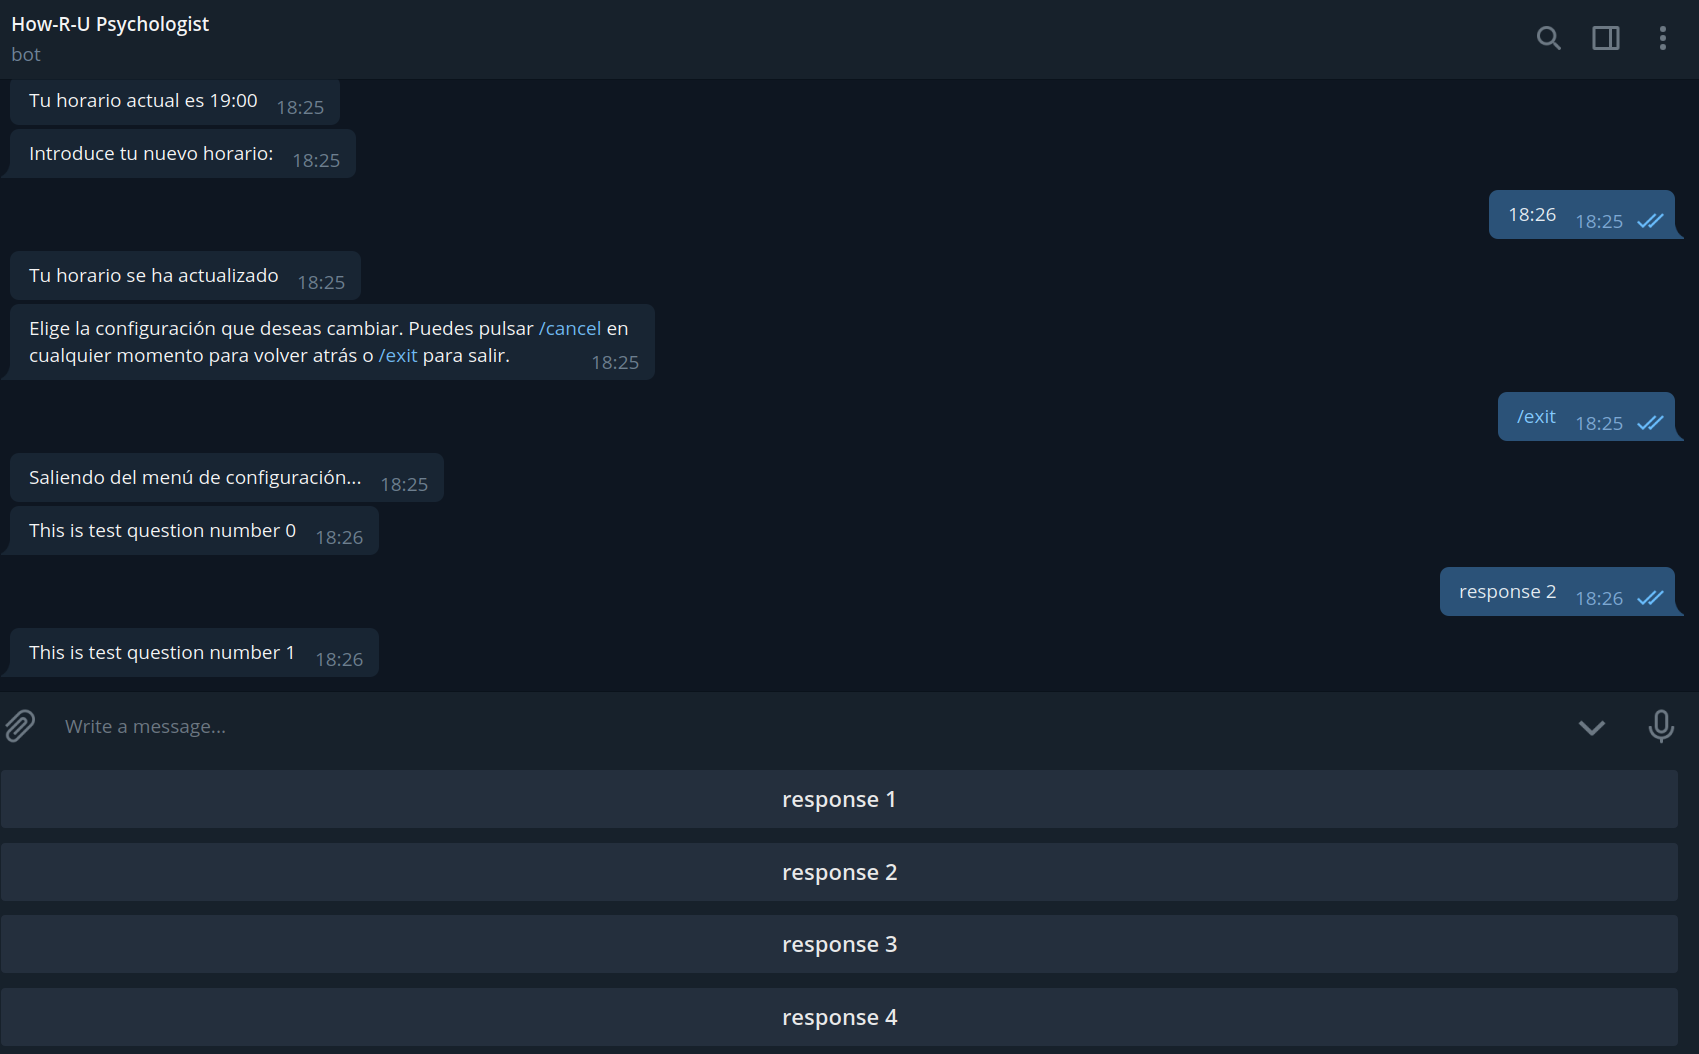
\includegraphics[width=\textwidth]{bot_answering.png}
  \caption{HOW-R-U converstional agent asking a question to a patient.}
\end{figure}

\begin{figure}[H]
  \centering
    
\includegraphics[width=\textwidth]{config_menu.png}
  \caption{Configurator menu.}
\end{figure}

The next conversational agent module is \emph{jobs}. Jobs are tasks that run a callback with a fixed frequency (daily, monthly, hourly, etc.,). In this project, jobs are used to ask the patient the corresponding questions when the schedule time arrives.

\begin{python}[caption={PendingQuestion job}, captionpos=b]
class PendingQuestionJob(object):
  def __init__(self, context, patient):
      self.patient = patient
      self._create_job(context)
  def job_callback(self, context):
      """
      Prompts PendingQuestions to the user.
      """
      pending_questions = self._get_pending_questions()
      for task in pending_questions:
          if not self.is_question_answered(task):
              question = task.question
              task.answering = True
              task.save()
              context.bot.send_message(chat_id=self.patient.identifier, text=question.text, reply_markup=keyboards.get_custom_keyboard(question.responses))
              while not self.is_question_answered(task):
                  time.sleep(0.5)
      message = messages[self.patient.language]['finish_answering'] if self.answered_questions_today() else messages[self.patient.language]['no_questions']
      logger.info(f'User {self.patient.username} answered all the questions')
      context.bot.send_message(chat_id=self.patient.identifier, text=message, reply_markup=ReplyKeyboardRemove())
      time.sleep(0.1)
      if was_configurator_running(self.patient.identifier, context):
          logger.info(f'Reopening configurator for user {self.patient.username} id {self.patient.identifier}')
          context.bot.send_message(chat_id=self.patient.identifier,  text=messages[self.patient.language]['select_config'], reply_markup=keyboards.config_keyboard[self.patient.language])

  def _create_job(self, context):
      context.job_queue.run_daily(callback=self.job_callback, time=self.patient.schedule, name=f'{self.patient.identifier}_pending_questions_job')
\end{python}

When a PendingQuestionJob instance is created, a daily job is established (running at the patient schedule time). The job callback queries the PendingQuestions database and select the ones that should be answered (depending on their frequency and last answer) and orders it by priority, so that questions with lower priority are asked first. Then, it creates a custom keyboard with one button per response and sends the patient the question text as a message. Finally, when all questions have been answered, the job informs the user and opens the configurator if it was open. Sleep times have been added to make the process smoother.


\emph{pics} folder is a temporary directory where profile pictures are stored and then deleted after encoding them in base-64 to be uploaded to the database. \emph{log} contains a basic logging utility that shows useful information, such as time, process and thread. Finally, \emph{src} contains the main file which starts the bot service:

\begin{python}[caption={Bot file, the one that starts the service}, captionpos=b]
def main():
    logger.info("Started HOW-R-U psychologist")
    updater = Updater(token=bot_config.TOKEN, use_context=True)
    dispatcher = updater.dispatcher
    handlers = [start_handler, config_handler, question_handler]
    # Add handlers and error callback to dispatcher
    for handler in handlers:
        dispatcher.add_handler(handler)
    dispatcher.add_error_handler(error_callback)
    updater.start_polling()
    updater.idle()
\end{python}
\subsection{Web interface}
\label{sec:web_int}

HOW-R-U web interface is is a \emph{django} project based on \cite{appseed} that is structured into four main applications: app (the homepage), questions manager, patients manager and authentication (create users, modify passwords and login/logout functionalities).

The first page that is shown to the user is the login interface, with text boxes for user and password fields. The user can also register in the system with a button.

\begin{figure}[H]
  \begin{subfigure}[t]{0.4\textwidth}
    \centering
    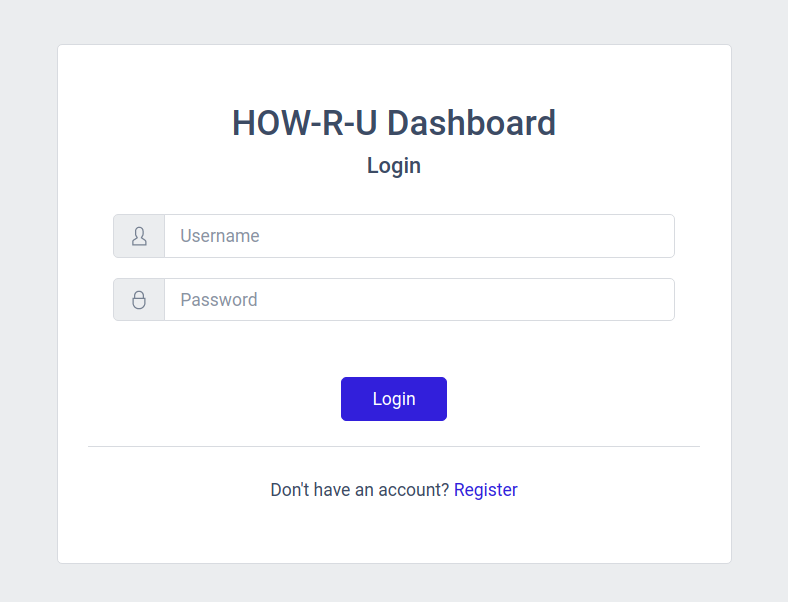
\includegraphics[width=\textwidth]{login.png}
  \end{subfigure}
  \hspace{3cm}
  \begin{subfigure}[t]{0.4\textwidth}
    \centering
    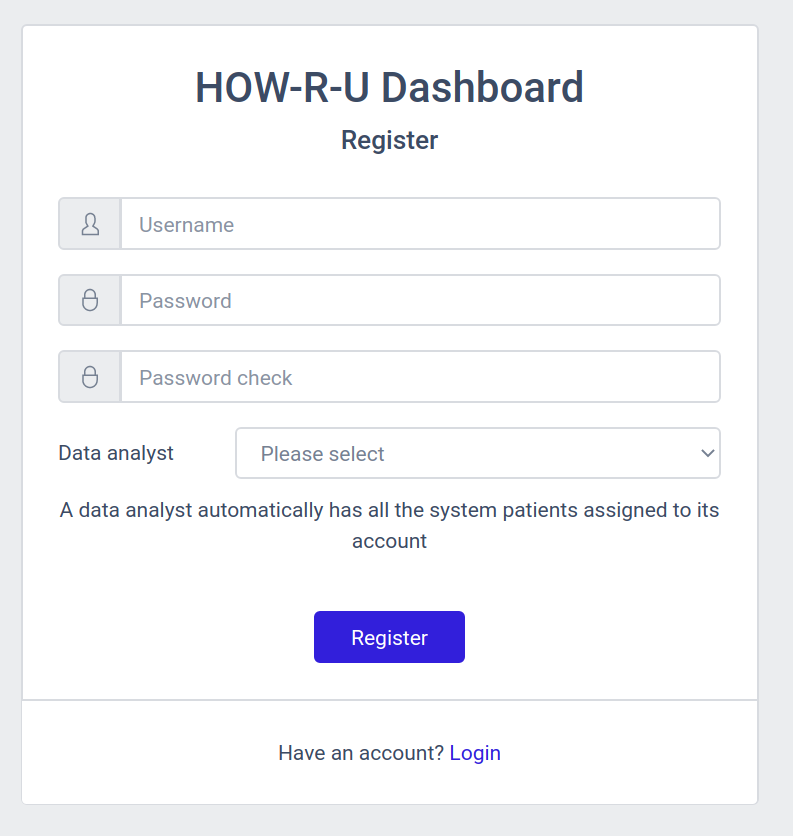
\includegraphics[width=\textwidth]{register.png}
  \end{subfigure}
  \caption{Login and register pages.}
\end{figure}


\begin{figure}[H]
    \centering
    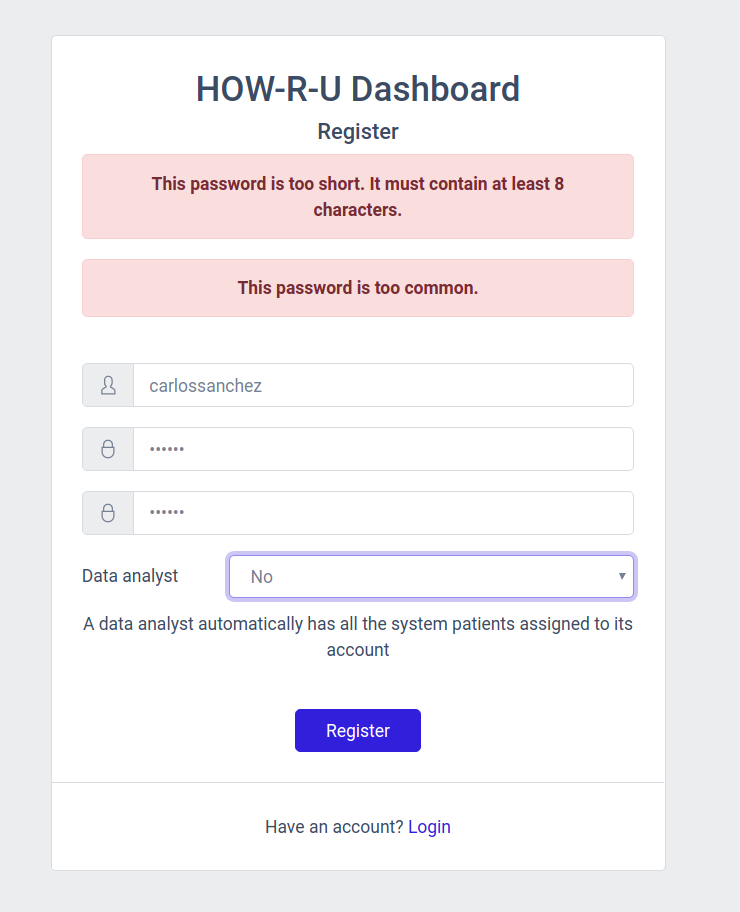
\includegraphics[width=0.5\textwidth]{register_error.png}
    \caption{Register form validations.}
\end{figure}

The register form has several validations, such as password length, strength, etc., These validators are provided by \emph{django auth} application. The user can also choose to be a \emph{data analyst}, a special user that does not have to add patients to their account manually. Everytime a patient registers into the system is automatically assigned to all data analysts. This feature is useful to collect statistics.

\begin{python}[caption={Method to register an user in the system}, captionpos=b]
  def register_user(request):
    if request.method == "POST":
        form = SignUpForm(request.POST)
        if form.is_valid():
            form.save()
            # If the doctor is an analyst, assign him/her all the patients in the system
            analyst = form.cleaned_data['is_analyst']
            form.instance.doctor.is_analyst = analyst
            if analyst:
                form.instance.doctor.patient_set.set(Patient.objects.all())
            form.save()
            username = form.cleaned_data.get("username")
            raw_password = form.cleaned_data.get("password1")
            user = authenticate(username=username, password=raw_password)
            login(request, user)
            return redirect("/")
    else:
        form = SignUpForm()
    return render(request, "accounts/register.html", {"form": form})
\end{python}

After logging in to the system, the homepage is shown. It is divided into three main sections. The first one shows statistics about the logged in doctor: the number of associated patients, submitted questions and total answers. Below, there is a panel that shows the percentage of answers per hour and patients per gender. Finally, a top 5 with the patients that have answered the most is exhibited.

\begin{figure}[H]
    \centering
    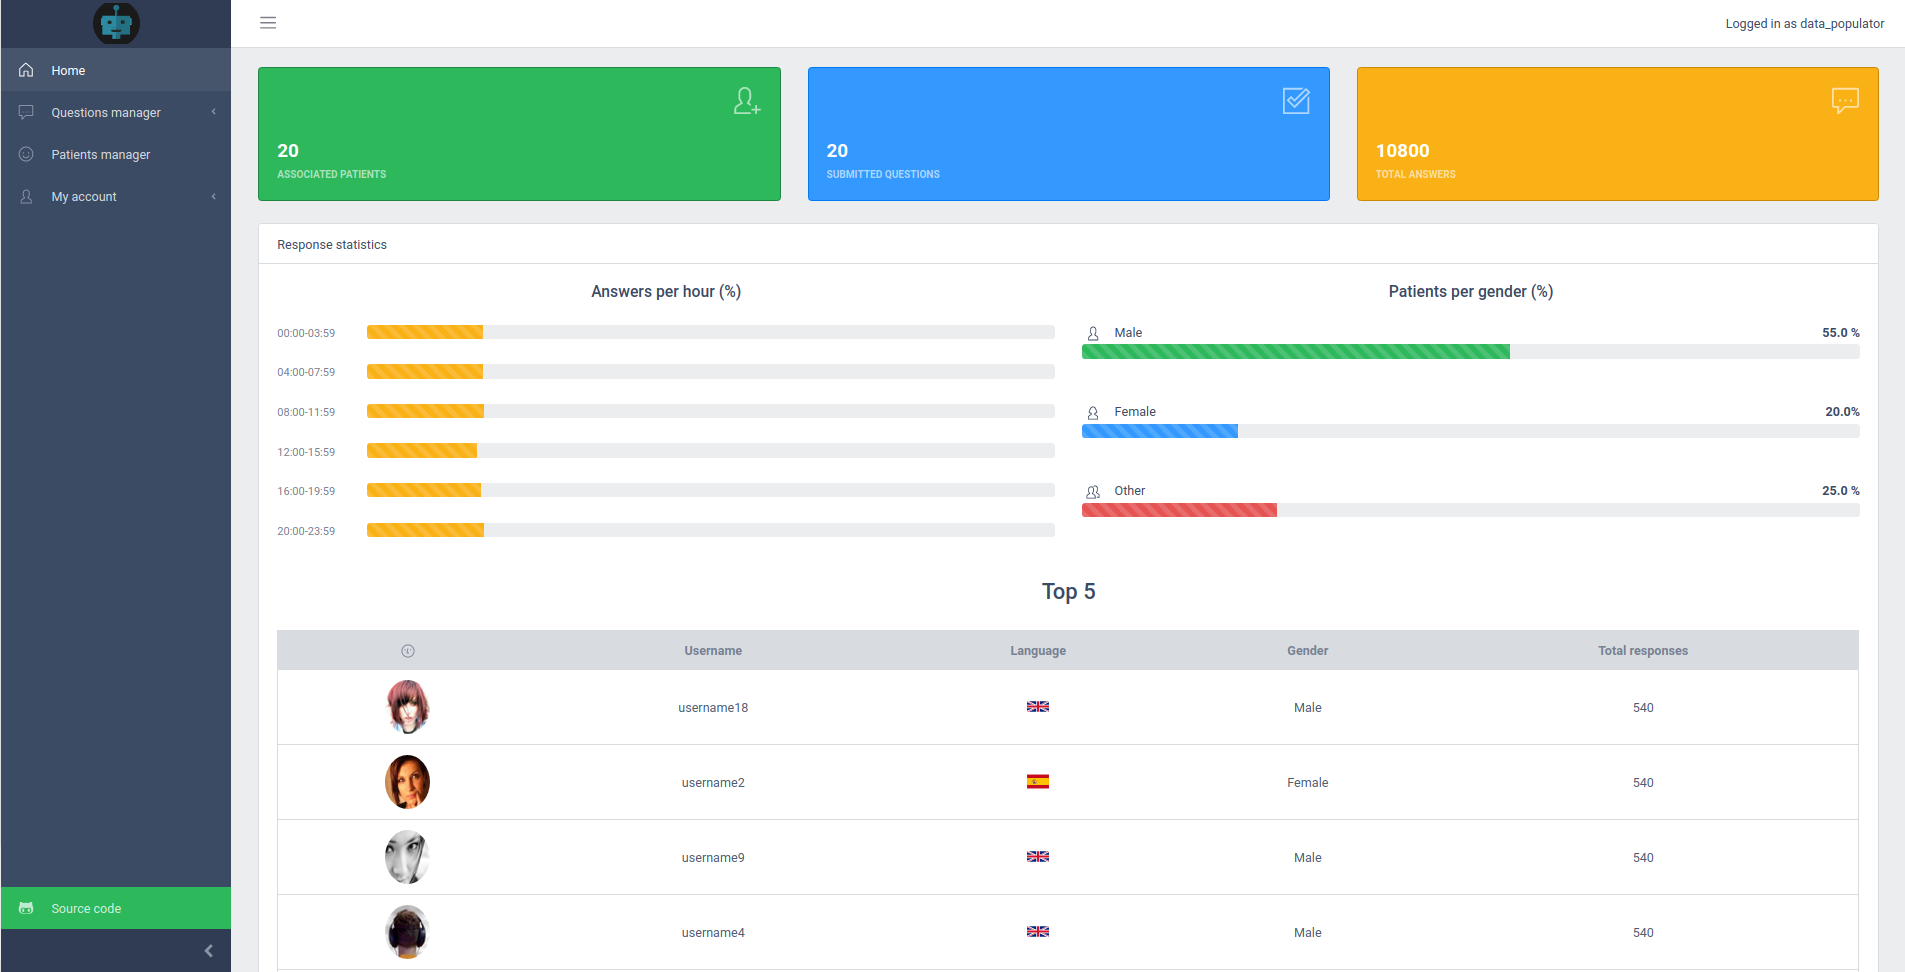
\includegraphics[width=0.8\textwidth]{homepage.png}
    \caption{HOW-R-U homepage.}
\end{figure}

\begin{figure}[H]
    \makebox[\linewidth]{
        
\includegraphics[width=0.8\linewidth]{homepage_1.png}
    }
    \caption{HOW-R-U homepage (doctor statistics).}
\end{figure}


\begin{figure}[H]
    \makebox[\linewidth]{
        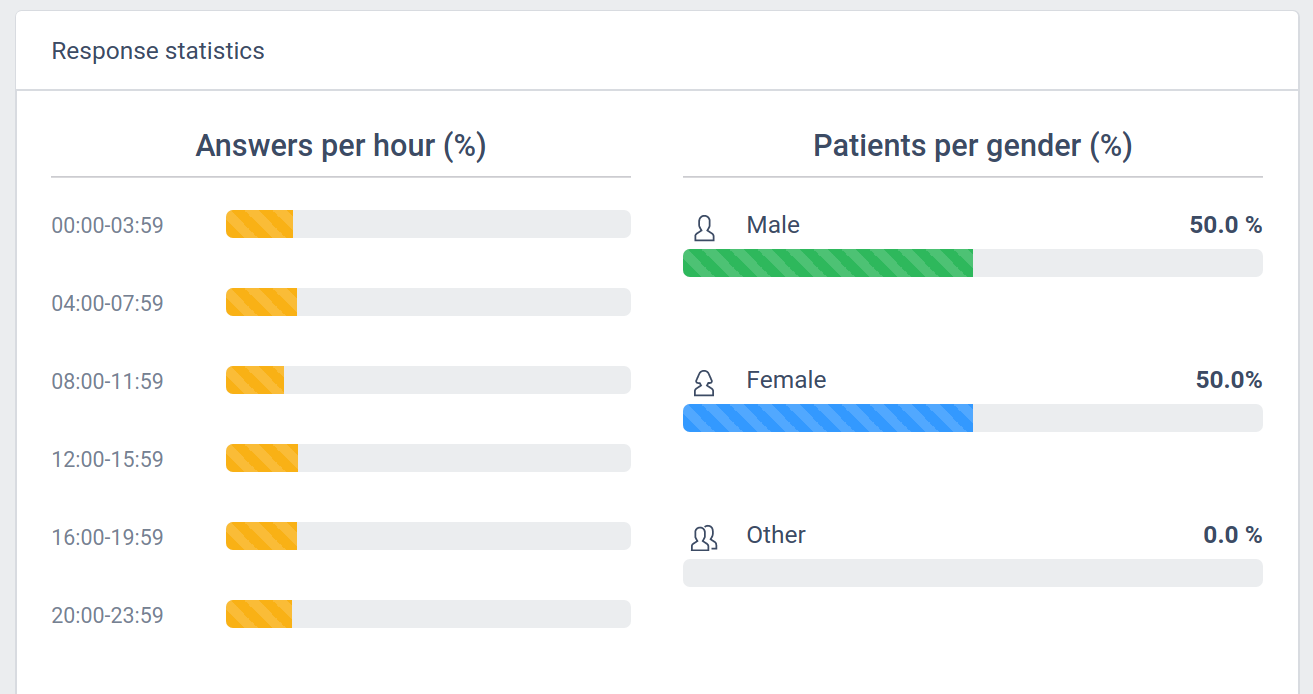
\includegraphics[width=0.8\linewidth]{homepage_2.png}
    }
    \caption{HOW-R-U homepage (response statistics).}
\end{figure}

\begin{figure}[H]
    \makebox[\linewidth]{
        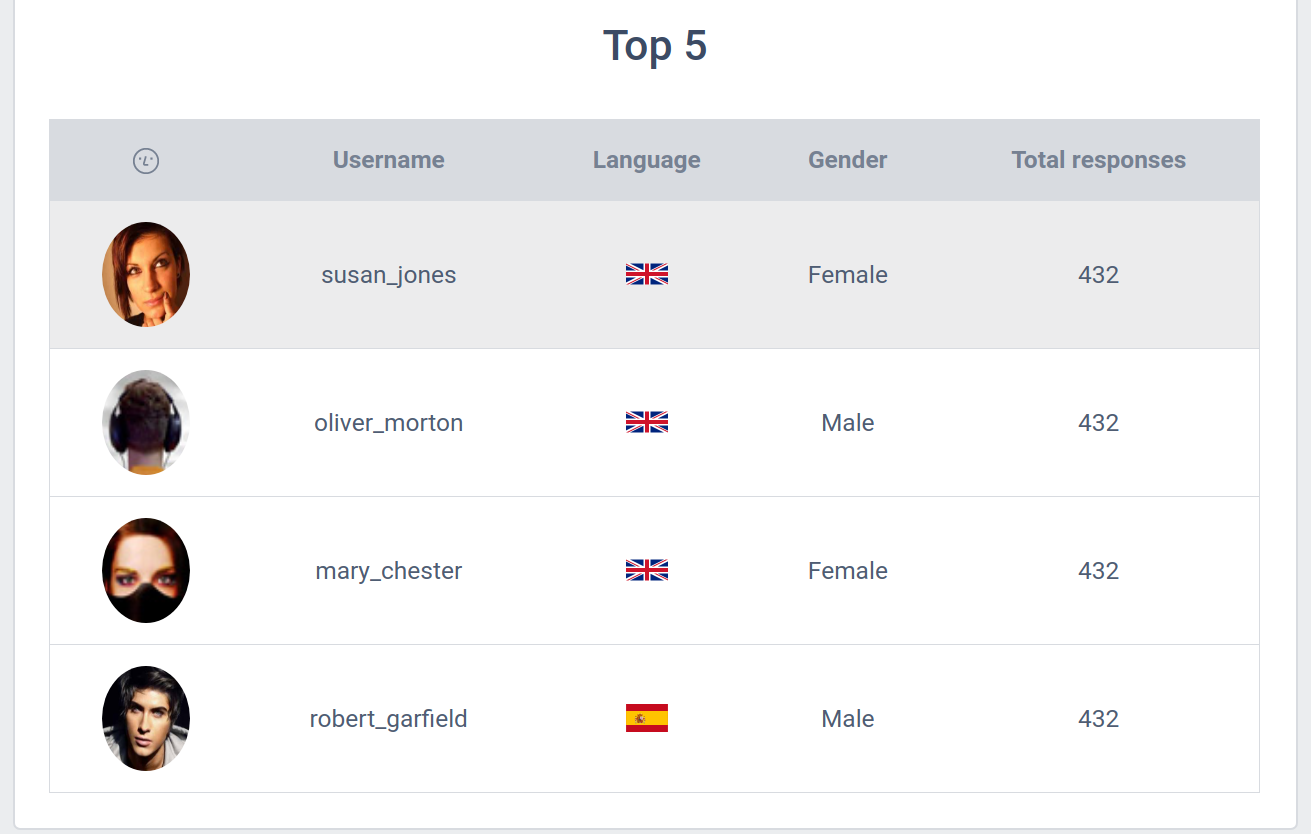
\includegraphics[width=\linewidth]{homepage_3.png}
    }
    \caption{HOW-R-U homepage (top 5).}
\end{figure}
\newpage
\begin{python}[caption={Method to show the main homepage components}, captionpos=b]
  @login_required(login_url="/login/")
  def index(request):
      """
      Shows the index page, including global parameters (top patients, number of associated patients, answers, gender and time percentages, etc.,)
      """
      doctor = request.user.doctor
      top_patients = get_top_patients(doctor)
      doctor_patients = doctor.patient_set
      number_associated_patients = doctor_patients.count()
      submitted_questions = Question.objects.filter(creator=doctor).count()
      total_answers = get_total_answers(doctor)
      male_percentage, female_percentage, other_percentage = get_gender_stats(doctor, number_associated_patients)
      answers_per_hour = get_answers_per_hour(doctor)
      context = {
          "top_patients": top_patients,
          "number_associated_patients": number_associated_patients,
          "submitted_questions": submitted_questions,
          "total_answers": total_answers,
          "male_percentage": male_percentage,
          "female_percentage": female_percentage,
          "other_percentage": other_percentage,
          "answers_per_hour": answers_per_hour
      }
      return render(request, "index.html", context)
\end{python}

In the sidebar the user has access to the main components of the system. The first one is the \textbf{questions manager}. When the doctor clics on it, a dropdown is opened, letting them choose public or private questions.

\begin{figure}[H]
    \centering
    
\includegraphics[width=0.25\textwidth]{questions_dropdown.png}
    \caption{Questions manager dropdown.}
\end{figure}

The public question interface shows a paginated table containing all the questions that have been incorporated into the system and marked as public. Moreover, there is a search bar and a button to add a public question to the user's questions list, so that he/she can assign it to the patients. When the user searches a question, the search term is encoded in the URL (GET request). The system has to build custom URLs when a search is being performed and the user clics the next page. This is achieved thanks to the code below.

\begin{figure}[H]
    \centering
    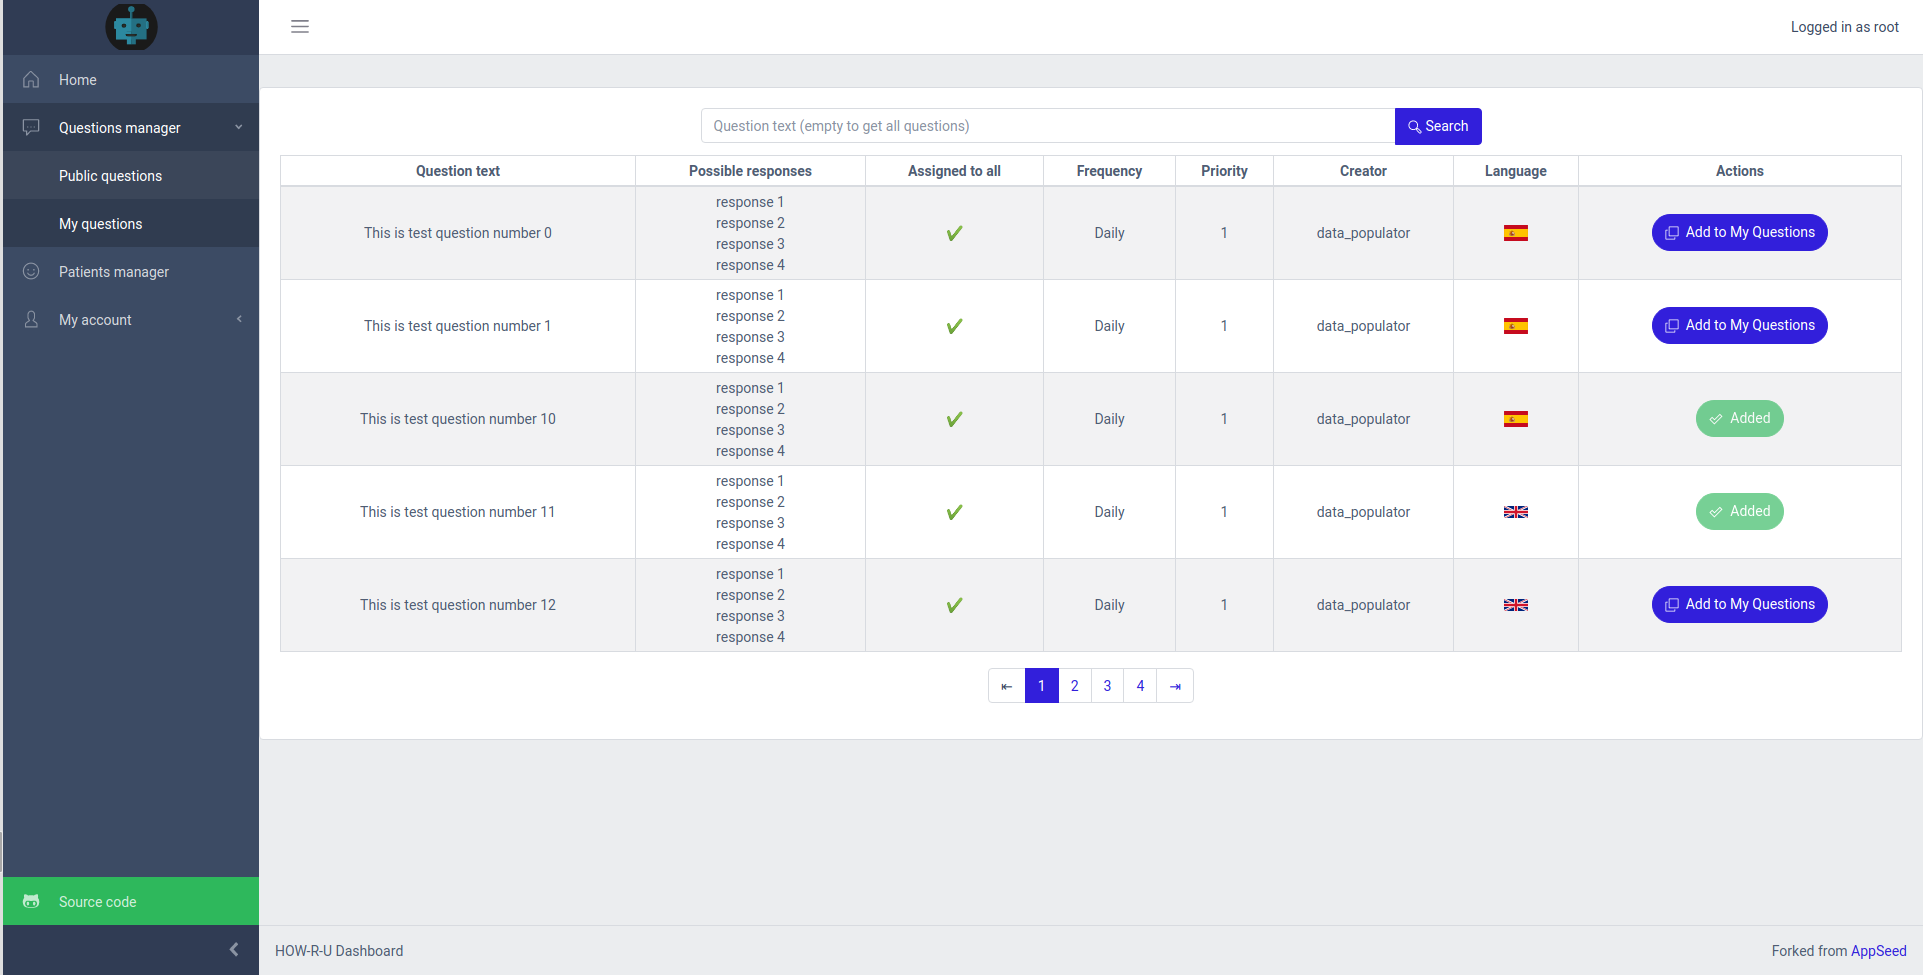
\includegraphics[width=\textwidth]{public_questions.png}
    \caption{Public questions page.}
\end{figure}

\begin{figure}[H]
    \makebox[\linewidth]{
        
\includegraphics[width=\linewidth]{public_questions_1.png}
    }
    \caption{Public questions page (question created by other user).}
\end{figure}

\begin{figure}[H]
    \makebox[\linewidth]{
        
\includegraphics[width=\linewidth]{public_questions_2.png}
    }
    \caption{Public questions page (question created by the current user).}
\end{figure}

\begin{python}[caption={Method to show public questions page}, captionpos=b]
  @login_required(login_url="/login/")
  def public_questions(request):
      """
      Shows public questions inside the system.
      """
      if 'search' in request.GET:
          term = request.GET['search']
          all_questions = Question.objects.filter(text__icontains=term, public=True).order_by('text')
      else:
          all_questions = Question.objects.filter(public=True).order_by('text')
      page = request.GET.get('page', 1)
      paginator = Paginator(all_questions, settings.PAGE_SIZE)
      try:
          questions = paginator.page(page)
      except PageNotAnInteger:
          questions = paginator.page(1)
      except EmptyPage:
          questions = paginator.page(paginator.num_pages)
      request.session['public_questions_page'] = page
      return render(request, 'questions_manager/public_questions.html', context={
          'questions': questions,
          'success_msg': request.session.pop('message', None)
      })
\end{python}

The HTML page (template) to show the public questions is built following the pseudo-code below:
\begin{lstlisting}[language=html, caption={Pseudo-code to generate public questions template page}, captionpos=b]
<table>
<thead>
<tr>
<th>Question text</th>
<th>Possible responses</th>
<th>Assigned to all</th>
<th>Frequency</th>
<th>Priority</th>
<th>Creator</th>
<th>Language</th>
<th>Actions</th>
</tr>
</thead>

    <tr>
        <td>
          {{ question.text }}
        </td>
        <td>
          
          {{response}} <br>
          
        </td>
        <td>
          
          check_icon
          
          cross_icon
          
        </td>
        <td>
          {{ question.get_frequency_display }}
        </td>
        <td>
          {{ question.priority }}
        </td>
        <td>
          {{ question.creator.user.username }}
          
          (You)
          
        </td>
        <td>
          
          spanish_flag
          
          england_flag
          
        </td>
        <td>
          
          added_button
          
          add_button
          
        </td>
    </tr>
    
    </tbody>
</table>
\end{lstlisting}

\begin{python}[caption={Pagination code snippets. Retrieved from \href{https://medium.com/@sumitlni/paginate-properly-please-93e7ca776432}{https://medium.com/@sumitlni/paginate-properly-please-93e7ca776432}}, captionpos=b]
@register.filter
def paginate(paginator, current):
  num_pages = settings.PAGE_SIZE
  if paginator.num_pages > 2 * num_pages:
      start = max(1, current - num_pages)
      end = min(paginator.num_pages, current + num_pages)
      if end < start + 2 * num_pages:
          end = start + 2 * num_pages
      elif start > end - 2 * num_pages:
          start = end - 2 * num_pages
      if start < 1:
          end -= start
          start = 1
      elif end > paginator.num_pages:
          start -= (end - paginator.num_pages)
          end = paginator.num_pages
      pages = [page for page in range(start, end + 1)]
      return pages[:(2 * num_pages + 1)]
  return paginator.page_range

@register.simple_tag
def get_url(request, field, value):
    query_string = request.GET.copy()
    query_string[field] = value
    return query_string.urlencode()
\end{python}



The user's questions page is similar to the public ones. The main differences is that there are three new buttons: modify, delete and create new questions.

\begin{figure}[H]
    \centering
    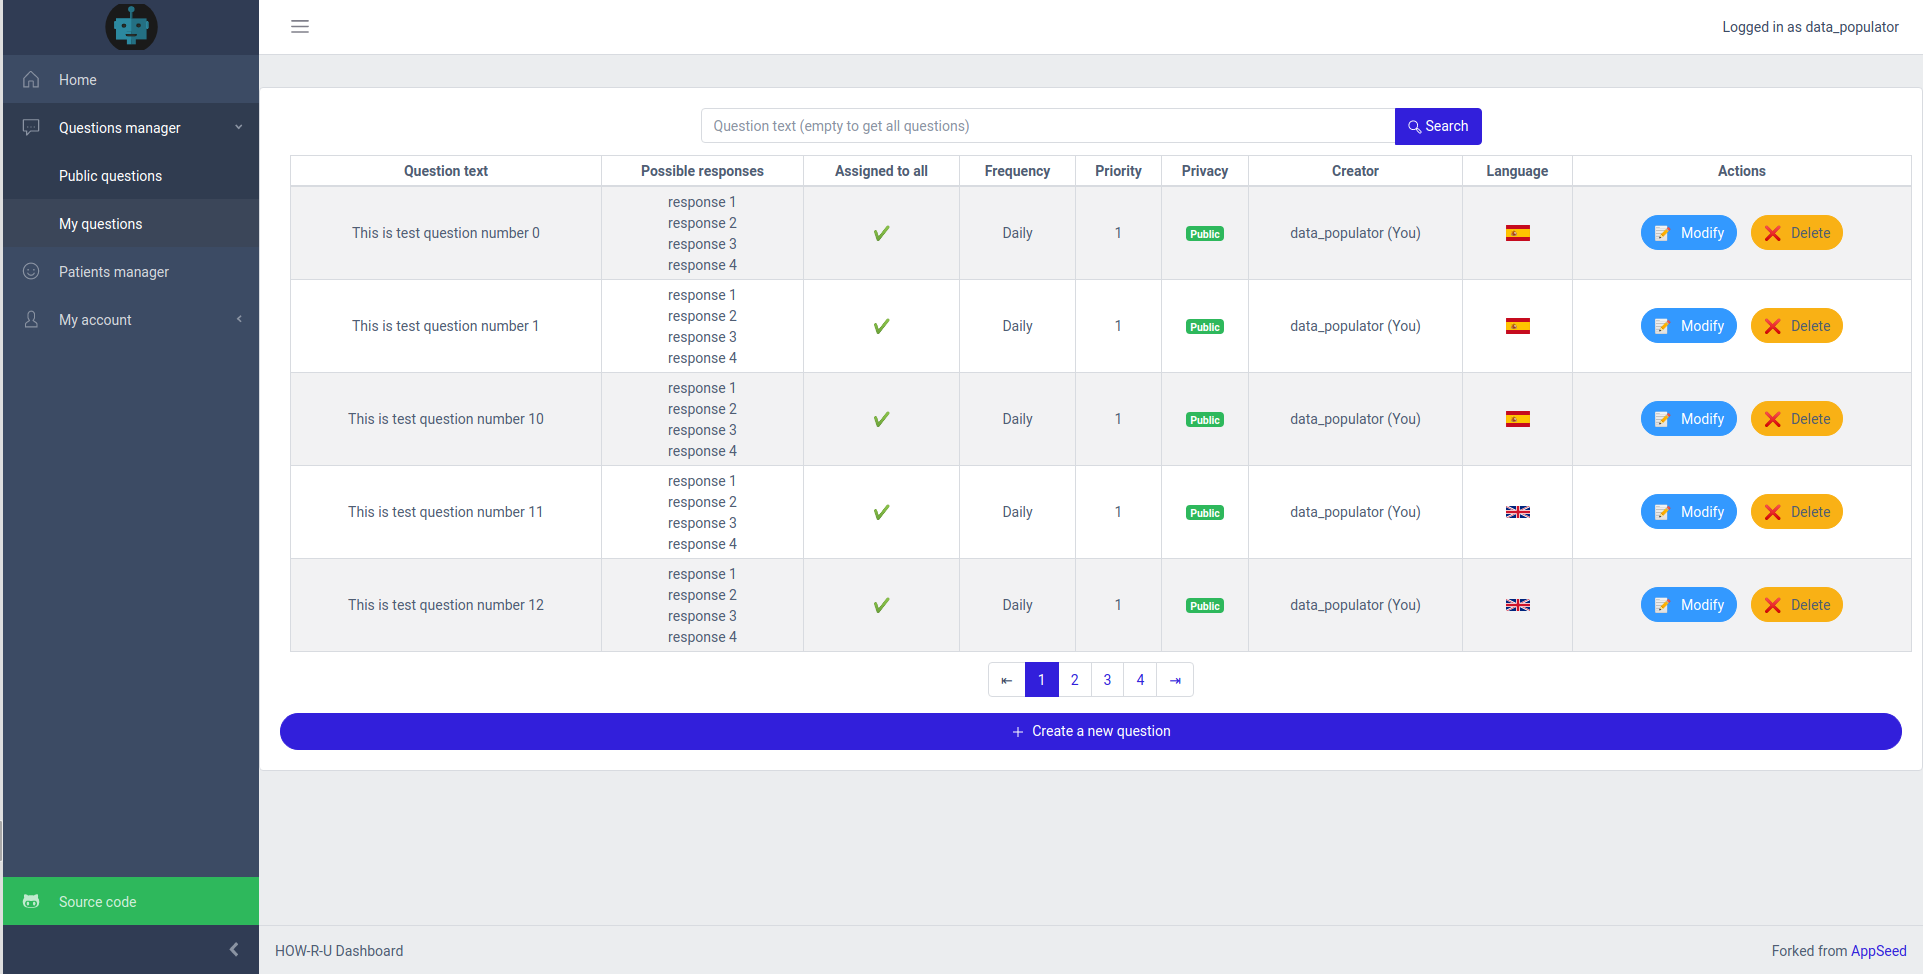
\includegraphics[width=\textwidth]{my_questions.png}
    \caption{User's questions page.}
\end{figure}


\begin{figure}[H]
    \makebox[\linewidth]{
        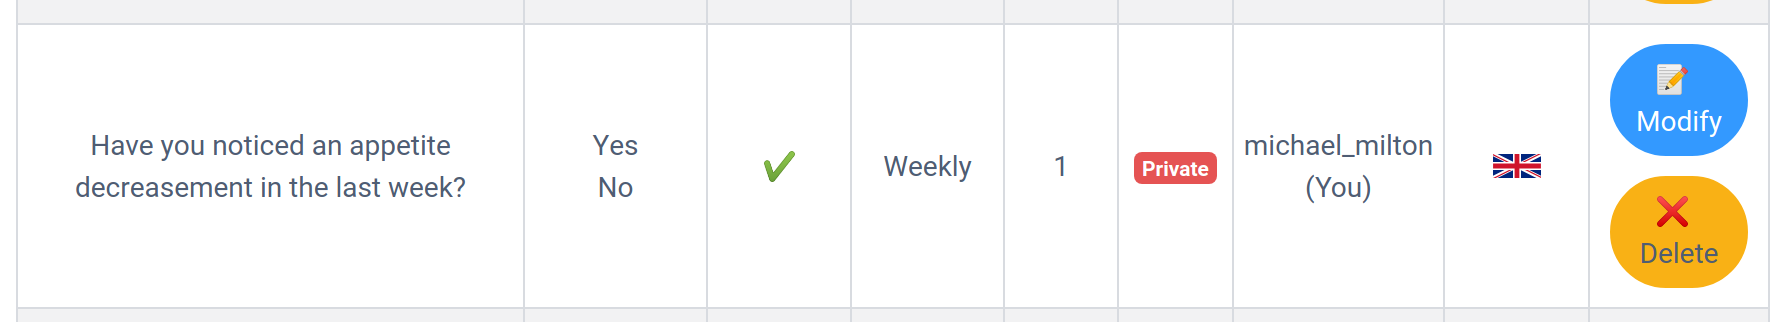
\includegraphics[width=\linewidth]{my_questions_1.png}
    }
    \caption{User's questions page (example).}
\end{figure}

The create and modify interfaces show a form with help messages to build or edit them. The main validations in these ones are that all fields are required and there should be at least two responses per question. Questions creator and modifier forms are created by inheritance from \emph{django.forms}.

\begin{figure}[H]
  \centering
    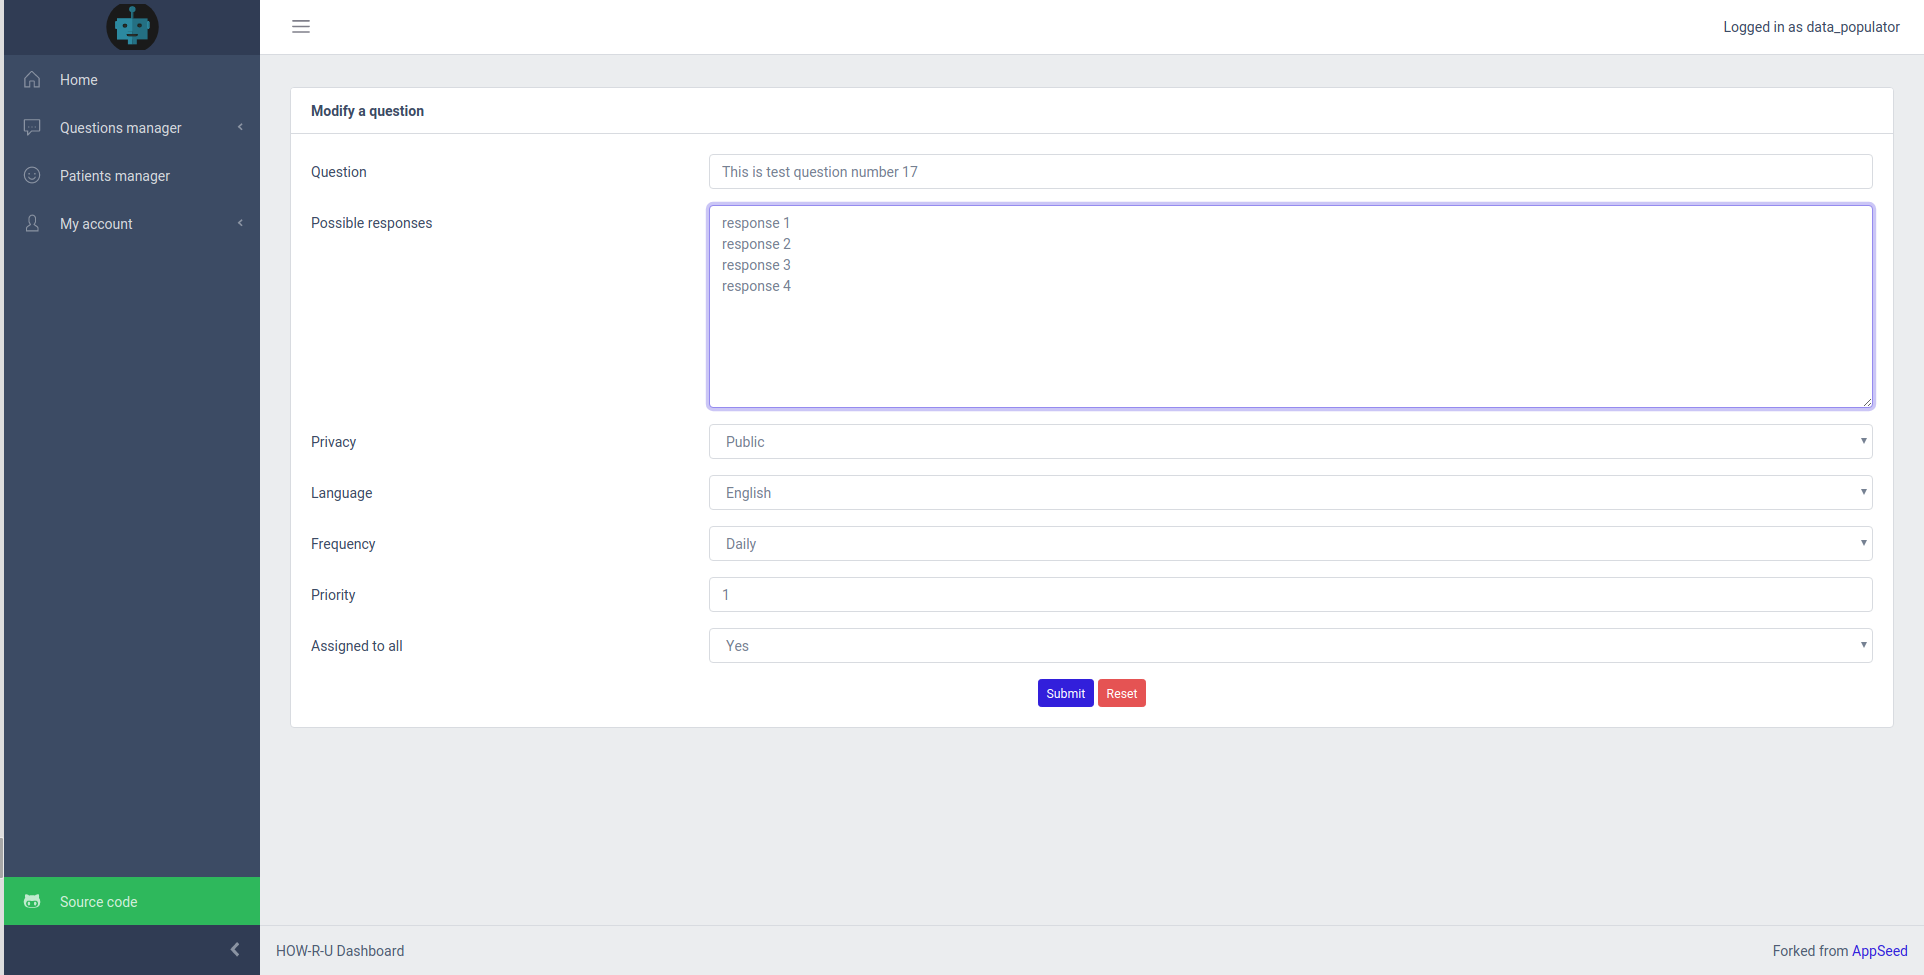
\includegraphics[width=\textwidth]{questions_modifier.png}
  \caption{Questions creator and modifier.}
\end{figure}

\begin{figure}[H]
    \makebox[\linewidth]{
        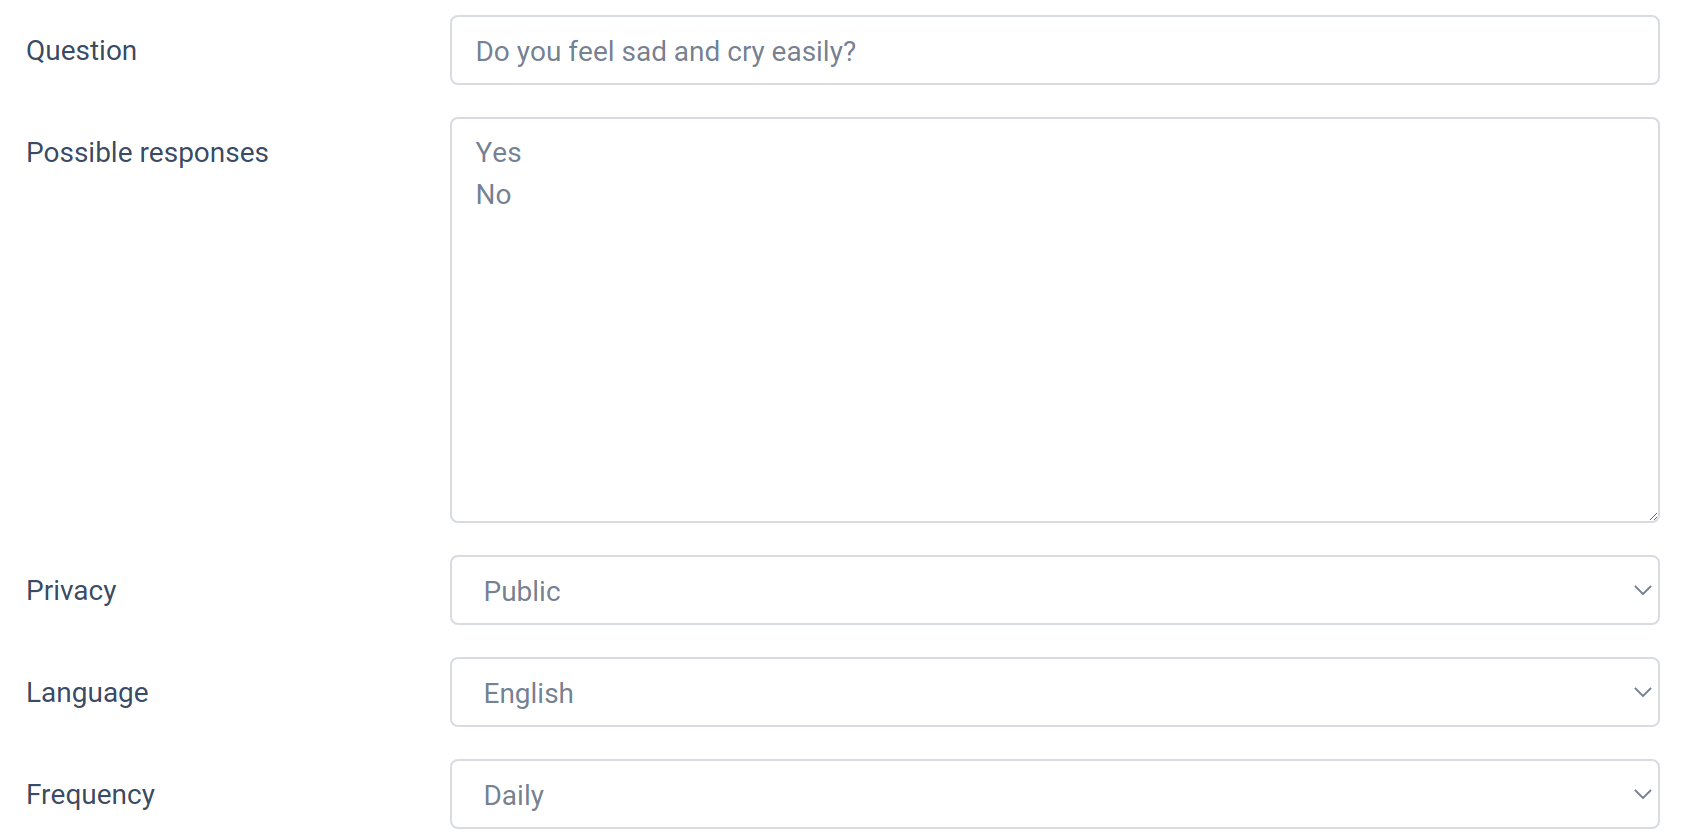
\includegraphics[width=\linewidth]{questions_modifier_1.png}
    }
    \caption{Questions creator and modifier fields (1/2).}
\end{figure}

\begin{figure}[H]
    \makebox[\linewidth]{
        
\includegraphics[width=\linewidth]{questions_modifier_2.png}
    }
    \caption{Questions creator and modifier fields (2/2).}
\end{figure}


The available fields for the Questions Creator are the following ones:
\begin{itemize}
  \item \textbf{Question text}: what should be asked to the patient.
  \item \textbf{Responses} (one per line). They should be ordered from bad to good so that plots are properly rendered.
  \item \textbf{Privacy} (public or private). Wether other users can add this question to their profile.
  \item \textbf{Language} (English or Spanish).
  \item \textbf{Frequency} (once, daily, weekly or mothly). How often the question should be asked.
  \item \textbf{Priority} ($[1,\infty[$). Order in which the question should be asked. Lower priority questions will be asked first.
  \item \textbf{Assigned to all} (yes or no). If set, the question will be automatically assigned to all the user's patients.
\end{itemize}

\begin{python}[caption={Form to create or modify questions}, captionpos=b]
class QuestionForm(ModelForm):
    privacy = forms.CharField()
    to_all = forms.CharField()
    responses_field = forms.CharField()
    class Meta:
        model = Question
        fields = ["text", "public", "language", "priority", "frequency"]
    def clean(self):
        cd = self.cleaned_data
        clean_responses = cd.get("responses_field").replace('\r', '')
        response_list = list()
        for response in clean_responses.split('\n'):
            if response:
                clean_response = response.strip()
                if clean_response:
                    response_list.append(response)
        if len(response_list) < 2:
            raise ValidationError("You must specify at least two possible responses")
        self.cleaned_data['responses'] = response_list
        privacy = cd.get("privacy")
        self.cleaned_data['public'] = privacy == "Public"
        self.cleaned_data['assigned_to_all'] = self.cleaned_data['to_all'] == "yes"
\end{python}

As \emph{public} and \emph{assigned to all} are boolean in the models but text in the views, we have to manually analyse the data retrieved from the form. The number of answers is also validated in the \emph{clean} method.

Finally, the questions deletion page consists of a view showing a confirmation message and two buttons, \textbf{confirm} and \textbf{back}.
\\

The patients manager consists of another paginated table that shows all the patients associated to the doctor. There is also a search bar, a button to add new patients and three buttons to manage each patient: view data, assign questions and delete patient from the doctor's page. Finally, there is also a export button to dump responses to a CSV file.

\begin{figure}[H]
  \centering
    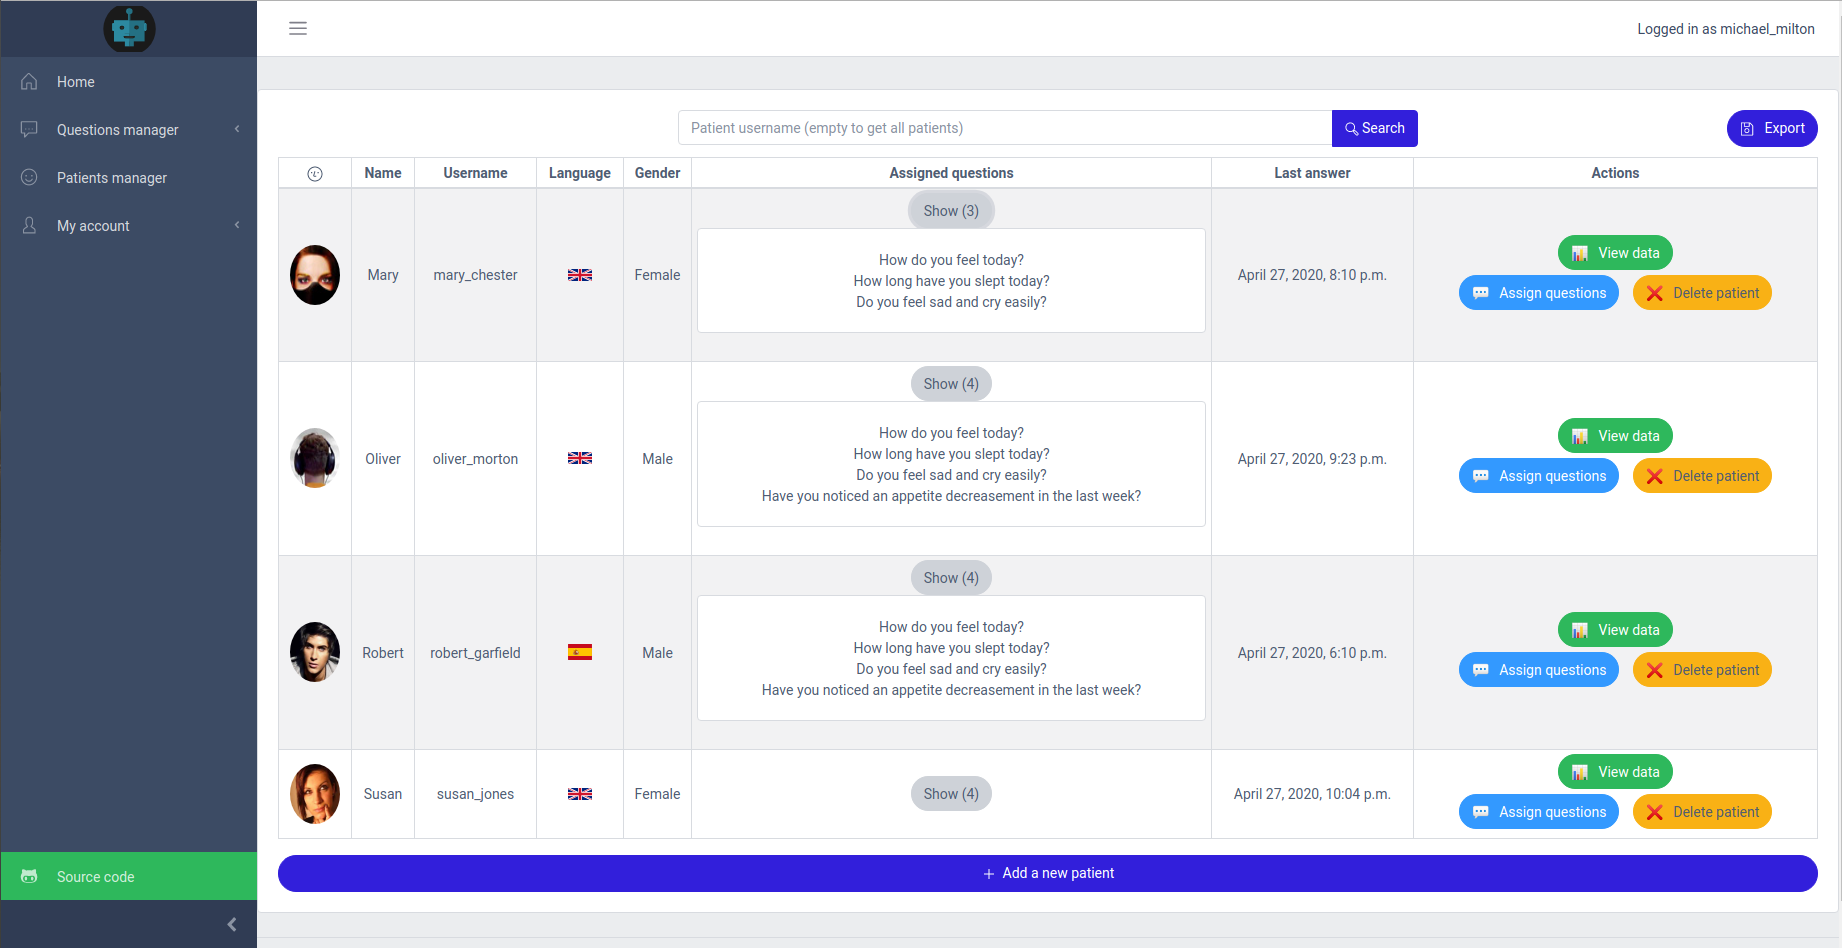
\includegraphics[width=\textwidth]{patients_manager.png}
  \caption{Patients manager.}
\end{figure}

\begin{figure}[H]
    \makebox[\linewidth]{
        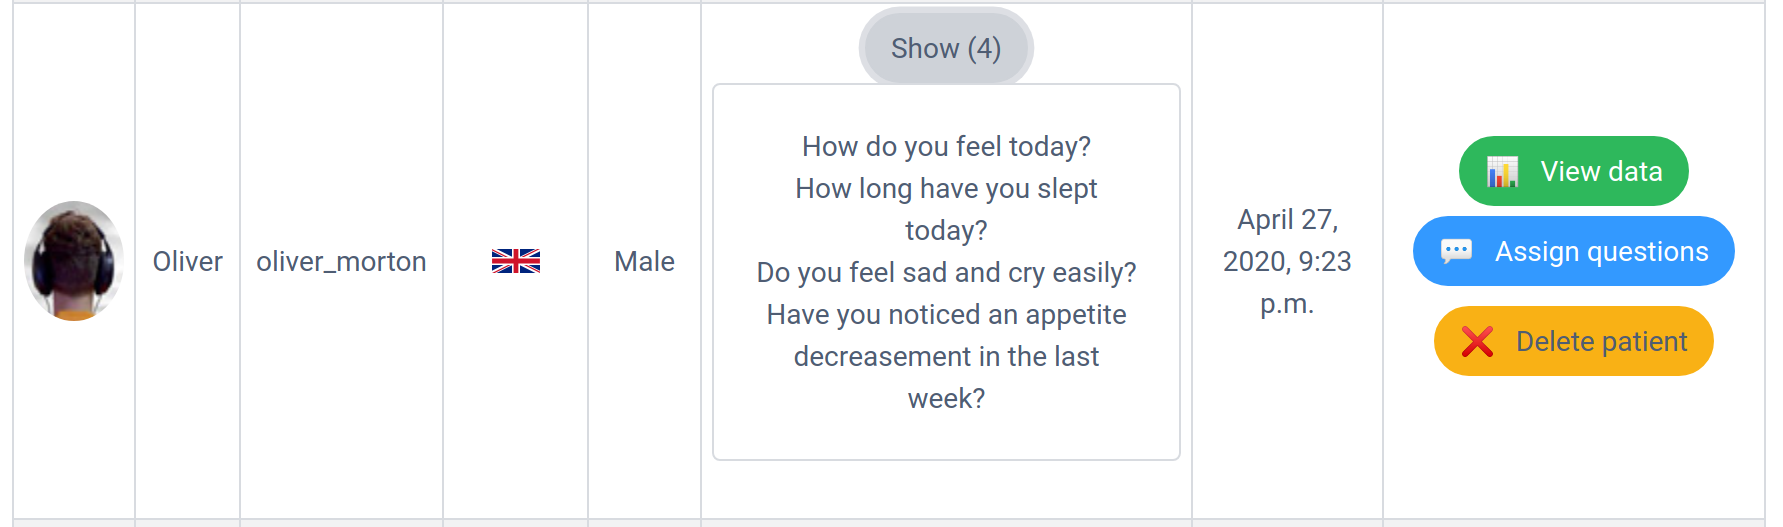
\includegraphics[width=0.8\linewidth]{patients_manager_1.png}
    }
    \caption{Patients manager (example).}
\end{figure}

The button to add new patients redirects the user to a page so that he/she can enter the patient's Telegram username. Once done, the patient will be shown in the main view.

The assign question page consists of a paginated table showing the doctor's questions list. The assignment/unassignment is performed with a button at the end of each row. These processes consist on creating or deleting a \emph{PendingQuestion} object linking doctor, patient and question.

\begin{figure}[H]
  \centering
    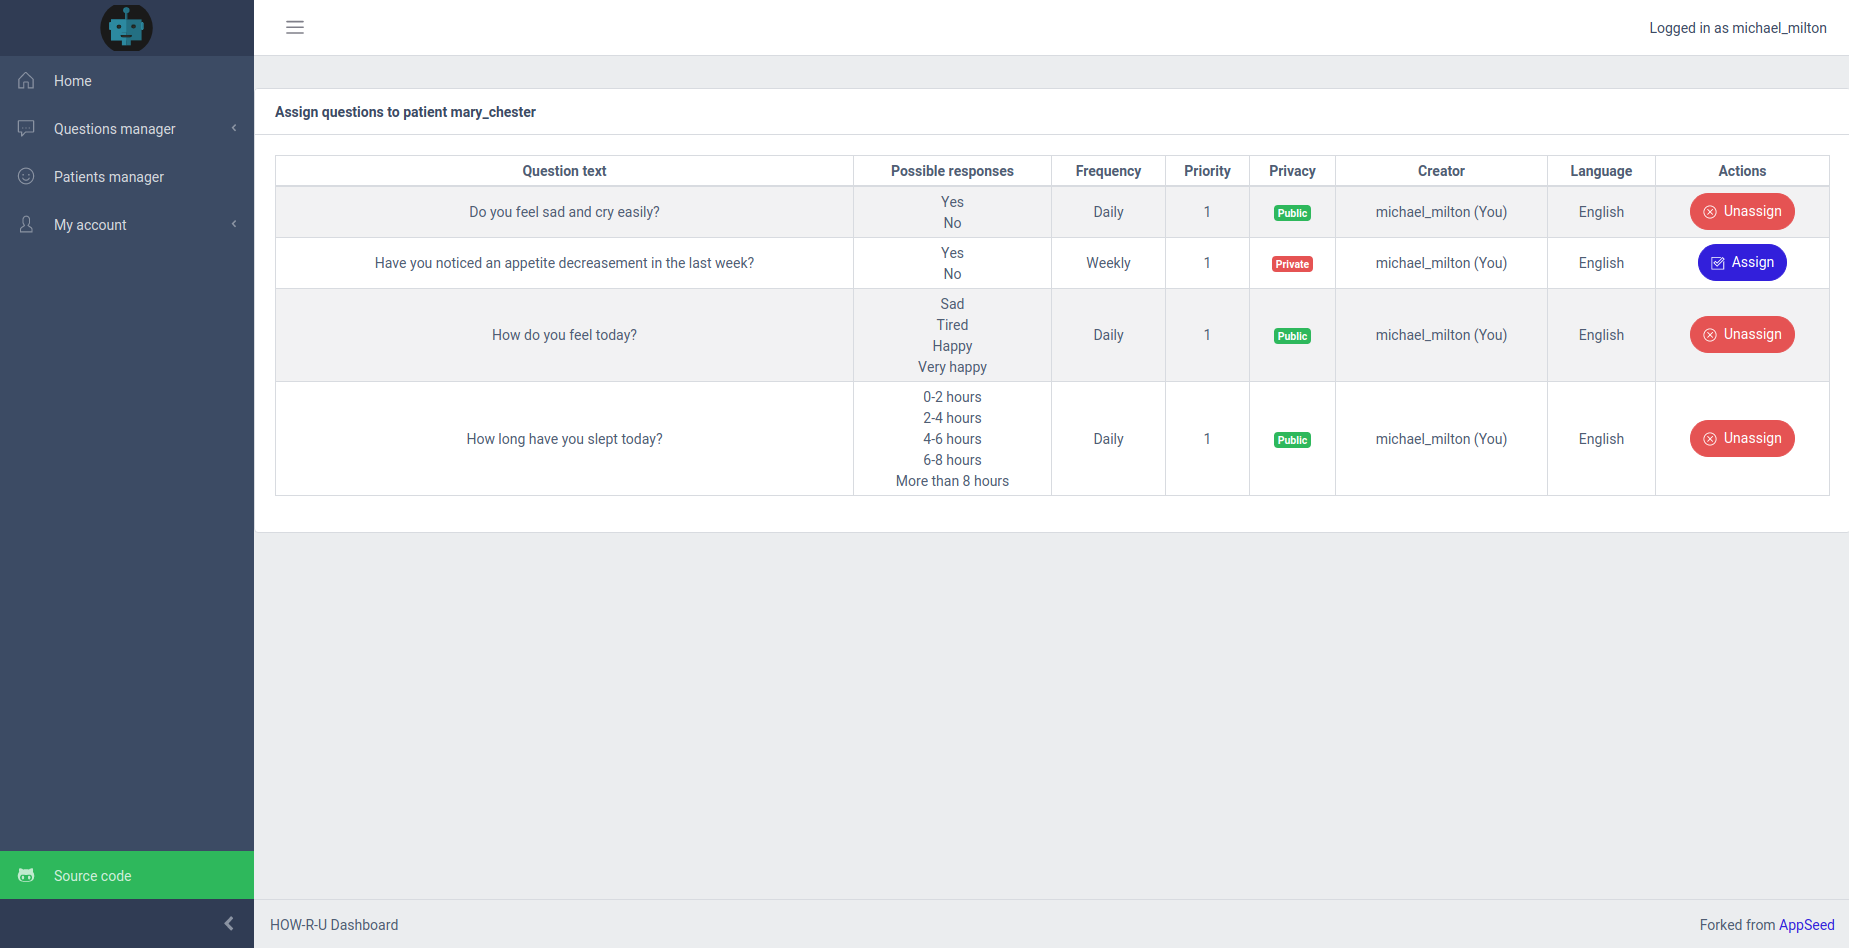
\includegraphics[width=\textwidth]{assign_questions.png}
  \caption{Patients manager assign questions page.}
\end{figure}

\begin{figure}[H]
    \makebox[\linewidth]{
        
\includegraphics[width=\linewidth]{assign_questions_1.png}
    }
    \caption{Patients manager assign questions page (unassigned question).}
\end{figure}

\begin{figure}[H]
    \makebox[\linewidth]{
        
\includegraphics[width=\linewidth]{assign_questions_2.png}
    }
    \caption{Patients manager assign questions page (assigned question).}
\end{figure}

The patients deletion button removes it from the doctor's associated patients list. After that, it can be added again. By deleting a patient, all the related \emph{PendingQuestion} are also deleted so that questions assigned to that user by the doctor that deletes it are asked no more. However, answers are preserved so that data can be analysed in the future if it is added again. If the users wants to delete this data, he/she must delete the patient account.
\\


The export page offers a form to select patients, start date and end date. When done, it generates a CSV file with four columns: patient username, question, answer and date.

\begin{figure}[H]
  \centering
    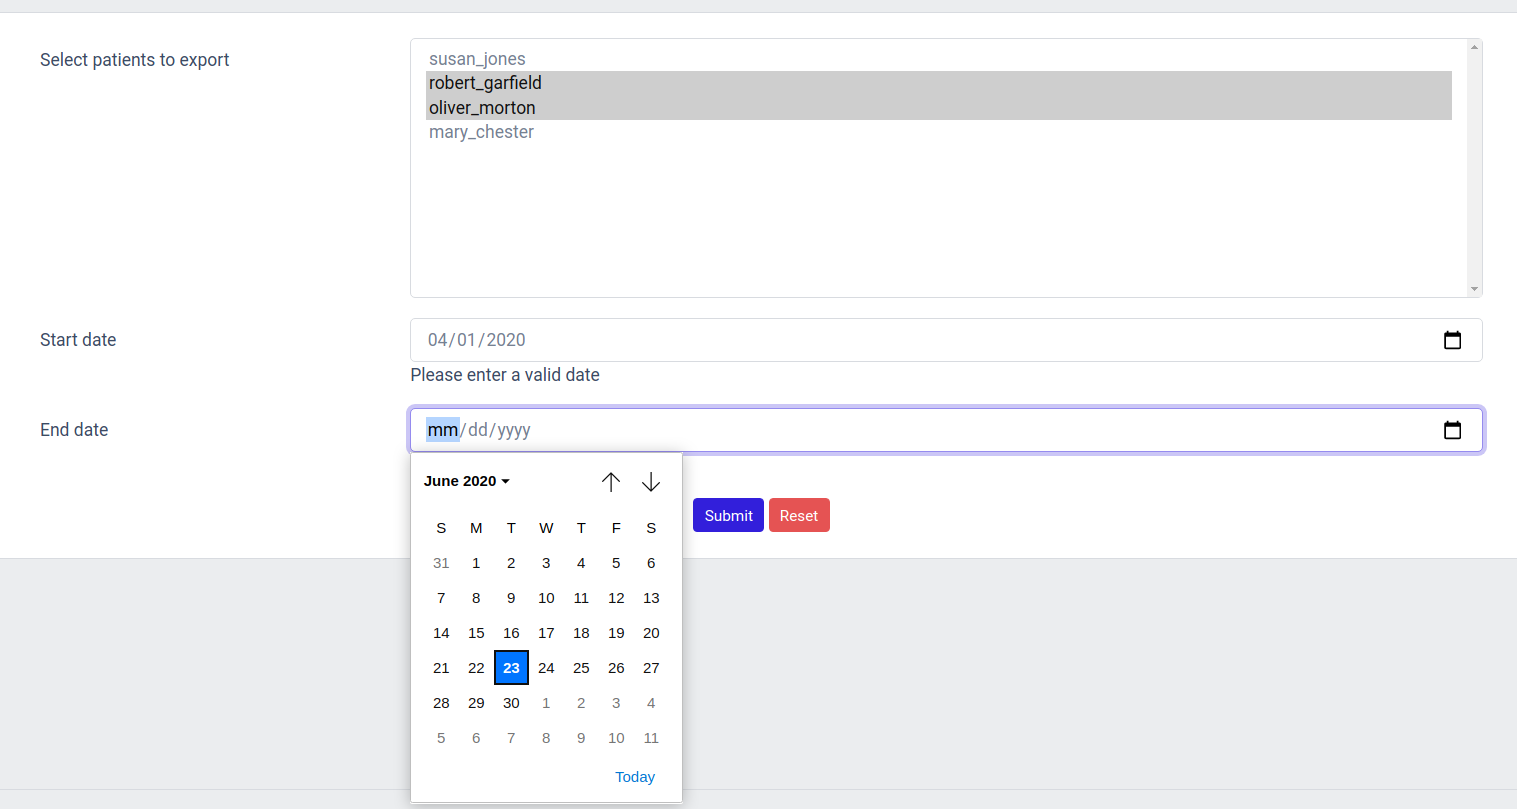
\includegraphics[width=\textwidth]{export.png}
  \caption{Export page}
\end{figure}

\begin{table}[h!]
\centering
\resizebox{\textwidth}{!}{%
\begin{tabular}{@{}cccc@{}}
\toprule
\textbf{Patient username} & \textbf{Question}                                                                                      & \textbf{Answer}   & \textbf{Date}       \\ \midrule
robert\_garfield          & How do you feel today?                                                                                 & Tired             & 2020-04-01 04:12:20 \\
robert\_garfield          & How do you feel today?                                                                                 & Sad               & 2020-04-02 05:24:20 \\
robert\_garfield          & How long have you slept today?                                                                         & 0-2 hours         & 2020-04-01 12:56:20 \\
robert\_garfield          & How long have you slept today?                                                                         & 4-6 hours         & 2020-04-02 11:28:20 \\
robert\_garfield          & Do you feel sad and cry easily?                                                                        & Yes               & 2020-04-01 14:22:21 \\
robert\_garfield          & Do you feel sad and cry easily?                                                                        & No                & 2020-04-02 06:31:21 \\
oliver\_morton            & How do you feel today?                                                                                 & Very happy        & 2020-04-01 01:45:19 \\
oliver\_morton            & How do you feel today?                                                                                 & Happy             & 2020-04-02 02:59:19 \\
oliver\_morton            & How long have you slept today?                                                                         & More than 8 hours & 2020-04-01 20:51:20 \\
oliver\_morton            & How long have you slept today?                                                                         & 2-4 hours         & 2020-04-01 22:24:20 \\
oliver\_morton            & Do you feel sad and cry easily?                                                                        & No                & 2020-04-01 07:47:20 \\
oliver\_morton            & Do you feel sad and cry easily?                                                                        & Yes               & 2020-04-02 17:26:20 \\
oliver\_morton            & \begin{tabular}[c]{@{}c@{}}Have you noticed an appetite \\ decreasement in the last week?\end{tabular} & Yes               & 2020-04-01 21:41:20 \\
oliver\_morton            & \begin{tabular}[c]{@{}c@{}}Have you noticed an appetite \\ decreasement in the last week?\end{tabular} & Yes               & 2020-04-08 21:09:20 \\ \bottomrule
\end{tabular}%
}
\caption{Example data generated with the \emph{Export} feature.}
\end{table}

Finally, the \emph{View Data} section generates plots showing patient's answers. There are two plots per question: a line chart showing the different answers amongst time and a pie one manifesting the number of times each answer has been replied. Both charts are interactive so that when the doctor hovers the mouse on them, a box is shown specifying more data about the selected section. The View Data page is also paginated and includes a search bar to filter questions.

\begin{figure}[H]
  \centering
    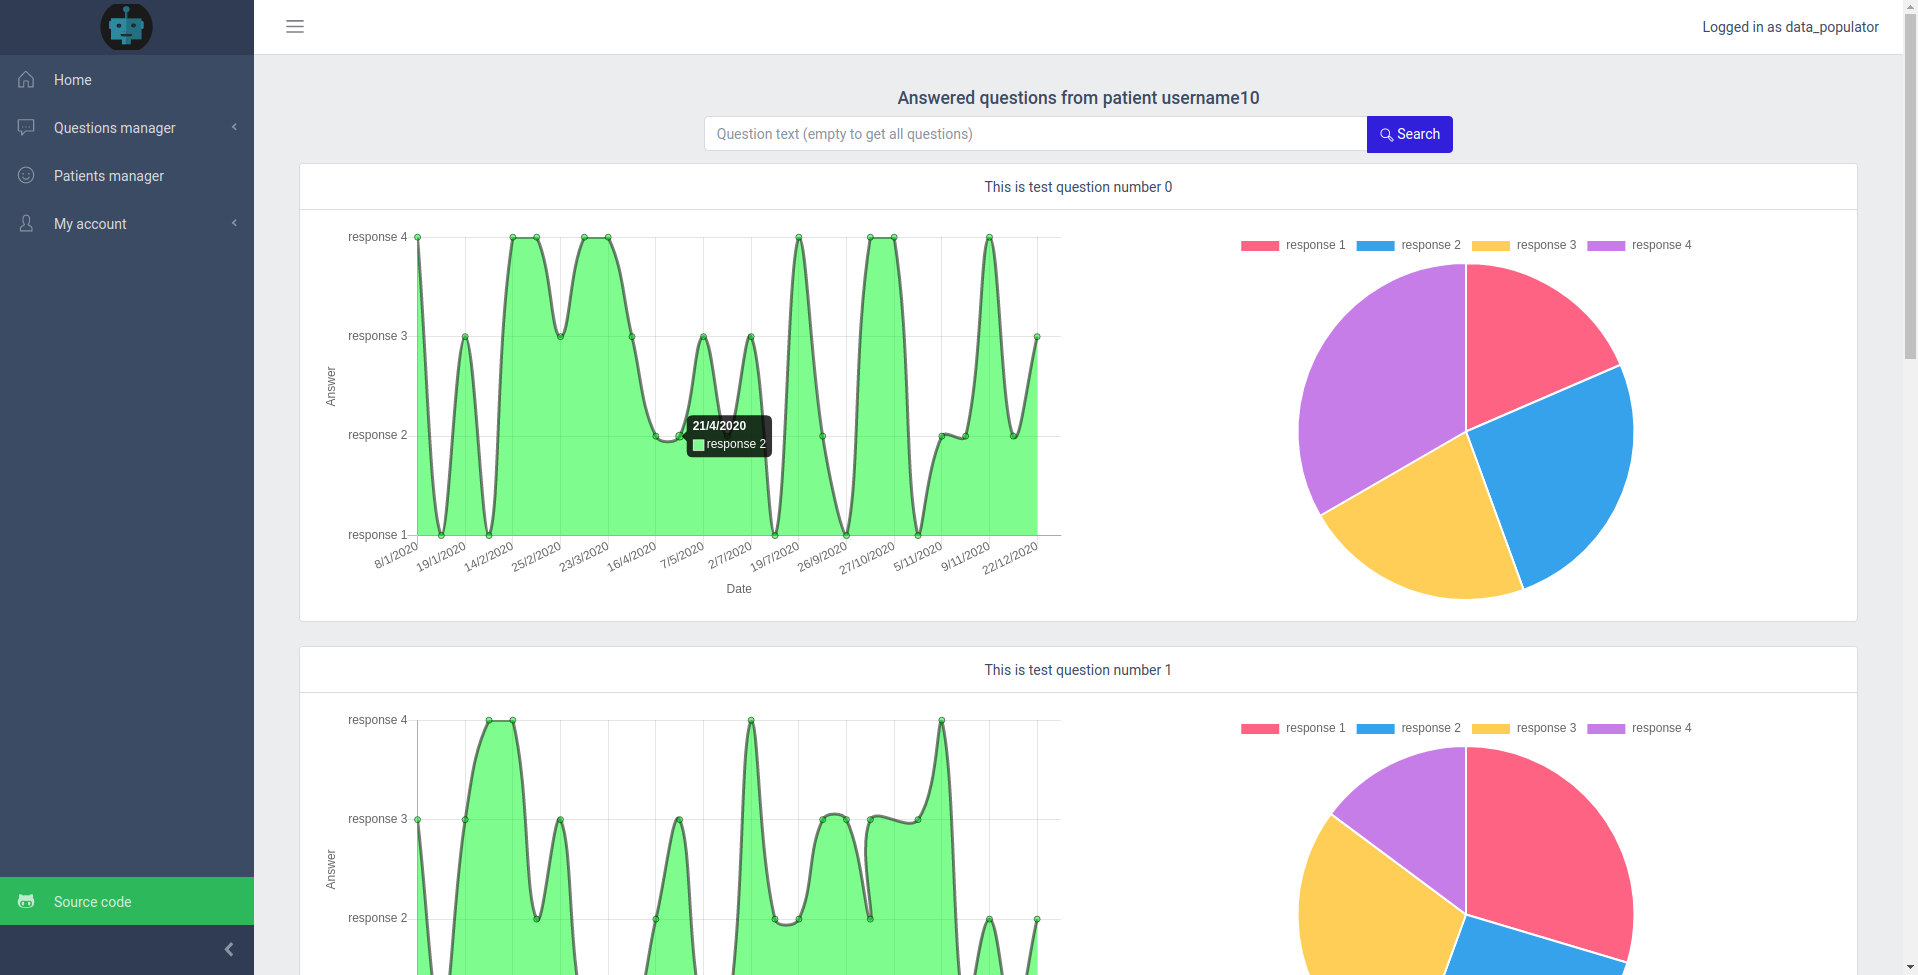
\includegraphics[width=\textwidth]{view_data.png}
  \caption{View data page.}
\end{figure}
Figures 34 and 35 show an extended view of the generated charts for a given question: the line one and the pie one. Charts are interactive, so that if the user hovers the mouse over them, a tooltip box will pop, showing the date in the line chart and the response and number of times that it has been answered in the pie one.

\begin{figure}[H]
    \makebox[\linewidth]{
        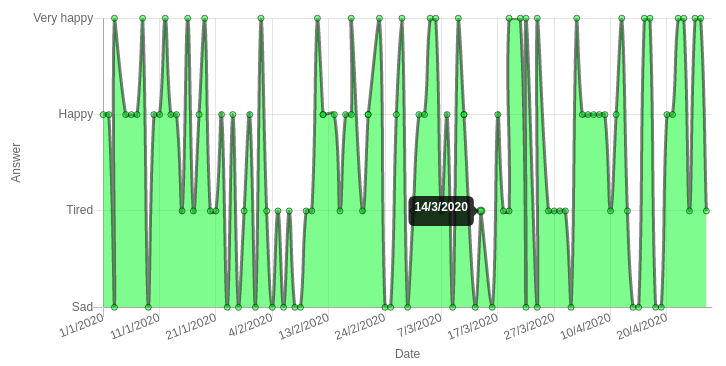
\includegraphics[width=\linewidth]{view_data_1.png}
    }
    \caption{View data page (line chart).}
\end{figure}

\begin{figure}[H]
    \makebox[\linewidth]{
        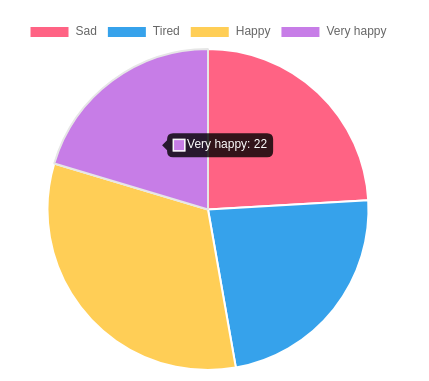
\includegraphics[width=0.5\linewidth]{view_data_2.png}
    }
    \caption{View data page (pie chart).}
\end{figure}

The last system view is the account manager, which consists of a dropdown that lets the user change the password, delete the account or log out.

\begin{figure}[H]
    \centering
    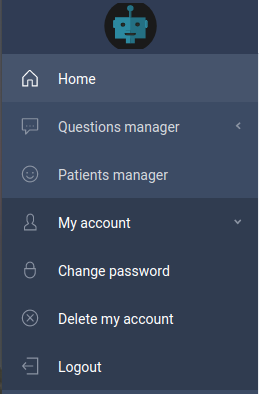
\includegraphics[width=0.3\textwidth]{account_dropdown.png}
    \caption{Account manager dropdown.}
\end{figure}

\begin{figure}[H]
    \centering
    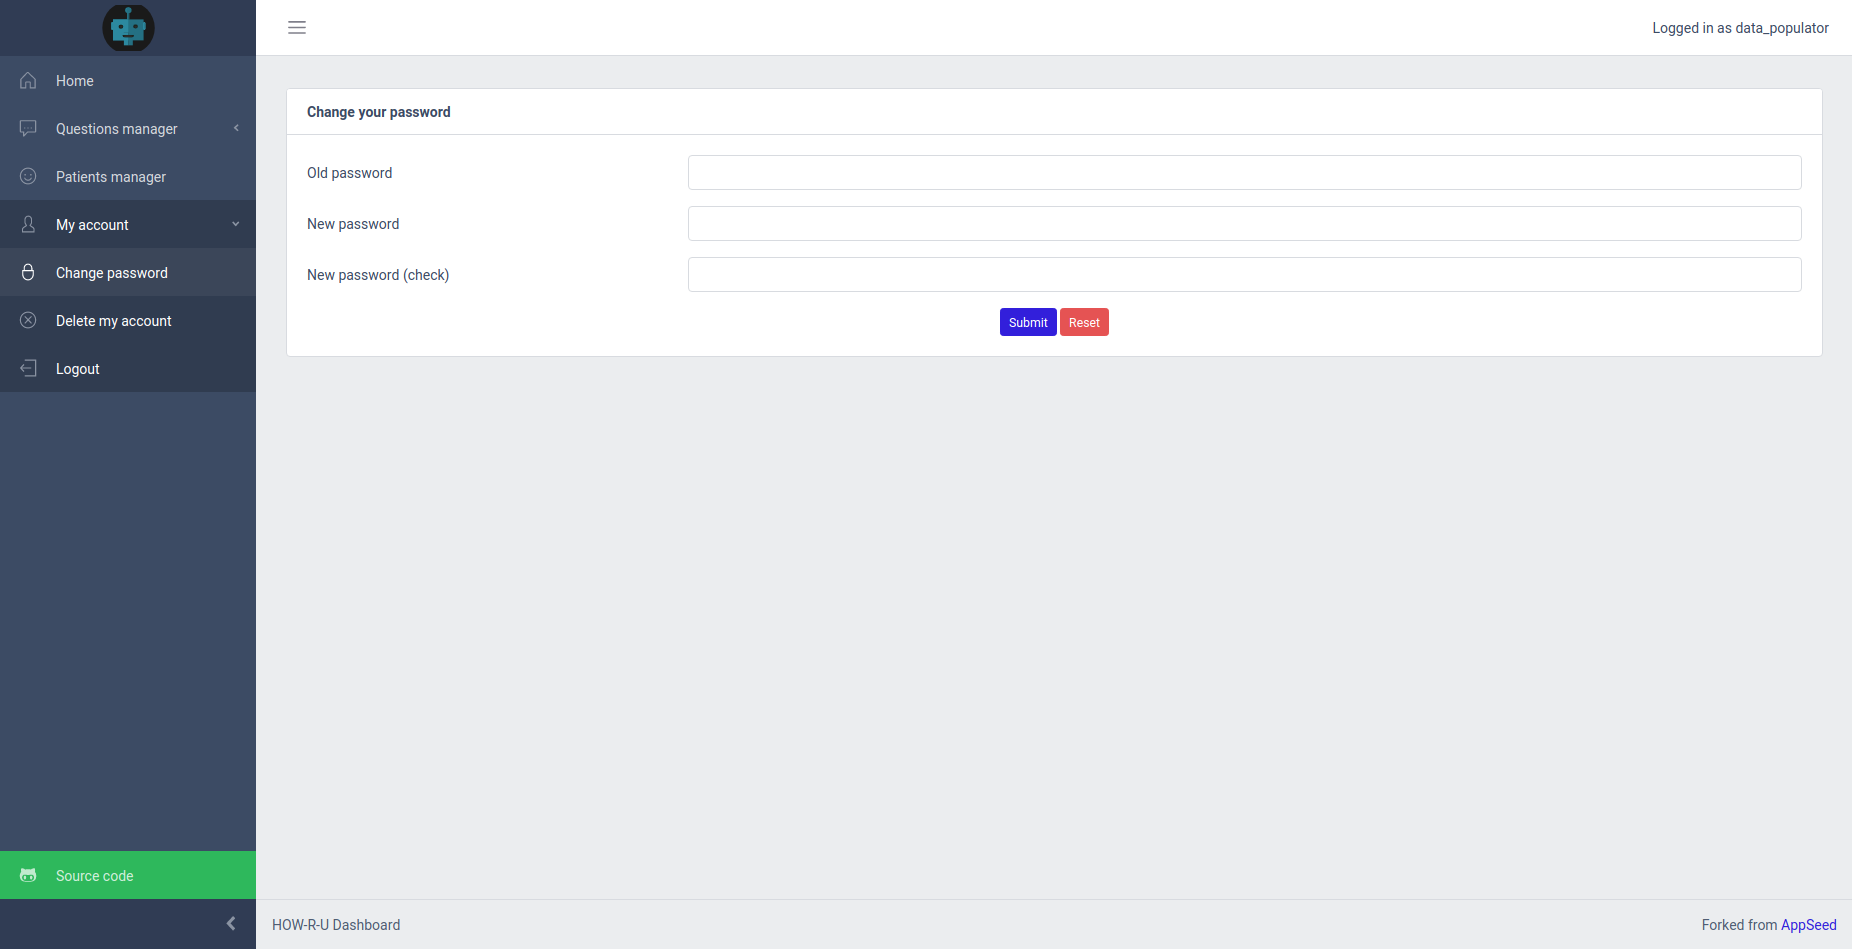
\includegraphics[width=0.7\textwidth]{change_pwd.png}
    \caption{Change password page.}
\end{figure}

\begin{python}[caption={Method to change user's password}, captionpos=b]
@login_required(login_url="/login/")
def change_password(request):
    """
    Allows an user to change his/her password
    """
    success = False
    if request.method == 'POST':
        form = PasswordChangeForm(request.user, request.POST)
        if form.is_valid():
            user = form.save()
            update_session_auth_hash(request, user)  # Important!
            success = True
    else:
        form = PasswordChangeForm(request.user)
    return render(request, 'change_password.html', {
        'form': form,
        'success': success
    })
\end{python}


\begin{figure}[H]
    \centering
    
\includegraphics[width=0.7\textwidth]{delete_account.png}
    \caption{Delete account page.}
\end{figure}


\begin{python}[caption={Method to delete an account}, captionpos=b]
@login_required(login_url="/login/")
def delete_account(request):
    """
    Deletes a doctor from the system
    """
    if request.method == "POST":
        request.user.doctor.delete()
        request.user.delete()
        return redirect('/')
    context = {}
    return render(request, 'delete_account.html', context)
\end{python}

HOW-R-U web interface icons have been gathered from \cite{pixabay}
\newpage
\subsection{Docker}
\label{sec:docker}

The HOW-R-U development environment is composed of four main containers: conversational agent, web interface, database and reverse proxy. The containers use volumes, so that changes made to their files take effect inmediately, avoiding an environment restart to test them. The \emph{docker-compose} specification is the following one:

\begin{lstlisting}[language=docker-compose-2, caption={HOW-R-U docker-compose file}, captionpos=b]
version: "3.1"
services:
  conversational-agent:
    image: conversational-agent
    links:
        - db:db
    volumes:
        - ~/Documents/TFG1920/howru/howru_chatbot:/opt/chatbot
    depends_on:
      - db
    restart: always
  db:
    image: postgres
    ports:
      - "5432:5432"
    environment:
      - POSTGRES_DB=postgres
      - POSTGRES_USER=postgres
      - POSTGRES_PASSWORD=postgres
    restart: always
  web-interface:
    image: web_interface
    links:
        - db:db
    volumes:
      - ~/Documents/TFG1920/howru/howru_web_interface:/opt/web_interface
    ports:
      - "8080:8080"
    depends_on:
      - proxy
      - db
    restart: always
  proxy:
    image: proxy
    ports:
      - "85:85"
    volumes:
      - ./proxy:/etc/nginx/conf.d
    restart: always
\end{lstlisting}

The individual \emph{Dockerfiles} of the previous containers are the following ones:

\begin{lstlisting}[language=docker, caption={HOW-R-U conversational agent Dockerfile}, captionpos=b]
FROM python:3.6.10-stretch

# Install requirements
ADD config/requirements.txt /root/requirements.txt
ADD config/routes.json /etc/howru/cfg/routes.json
RUN pip install -r /root/requirements.txt

# iPython for debugging
RUN pip3.6 install ipython

# Set PYTHONPATH
ENV PYTHONPATH /opt/chatbot

# Run bot
WORKDIR /opt/chatbot
CMD python3 manage.py makemigrations && \
    python3 manage.py migrate && \
    python3 src/bot.py
\end{lstlisting}

\begin{lstlisting}[language=docker, caption={HOW-R-U web interface Dockerfile}, captionpos=b]
FROM python:3.6.10-stretch
ENV PYTHONUNBUFFERED 1

# Copy config files
ADD config/requirements.txt /root/requirements.txt
ADD config/routes.json /etc/howru/cfg/routes.json
ADD config/initial_data.json /initial_data.json

# Install dependencies
RUN pip install -r /root/requirements.txt

# iPython for debugging
RUN pip3.6 install ipython

# Set workdir
WORKDIR /opt/web_interface

# Run server
CMD python3 manage.py makemigrations && \
    python3 manage.py migrate && \
    python3 manage.py loaddata /initial_data.json && \
    python3 manage.py runserver 0:8080
\end{lstlisting}

\begin{lstlisting}[language=docker, caption={HOW-R-U web reverse proxy Dockerfile}, captionpos=b]
FROM nginx:latest
COPY web_interface.conf /etc/nginx/conf.d/web_interface.conf
\end{lstlisting}

The reverse proxy configuration file just indicates the port where the web interface will be hosted:
\begin{lstlisting}[language=nginx, mathescape=false, caption={HOW-R-U web reverse proxy configuration file}, captionpos=b]
server {
    listen      85;
    location / {
        proxy_pass http://localhost:8080/;
        proxy_set_header Host $host;
        proxy_set_header X-Forwarded-For $proxy_add_x_forwarded_for;
    }
}
\end{lstlisting}

\begin{figure}[H]
  \centering
  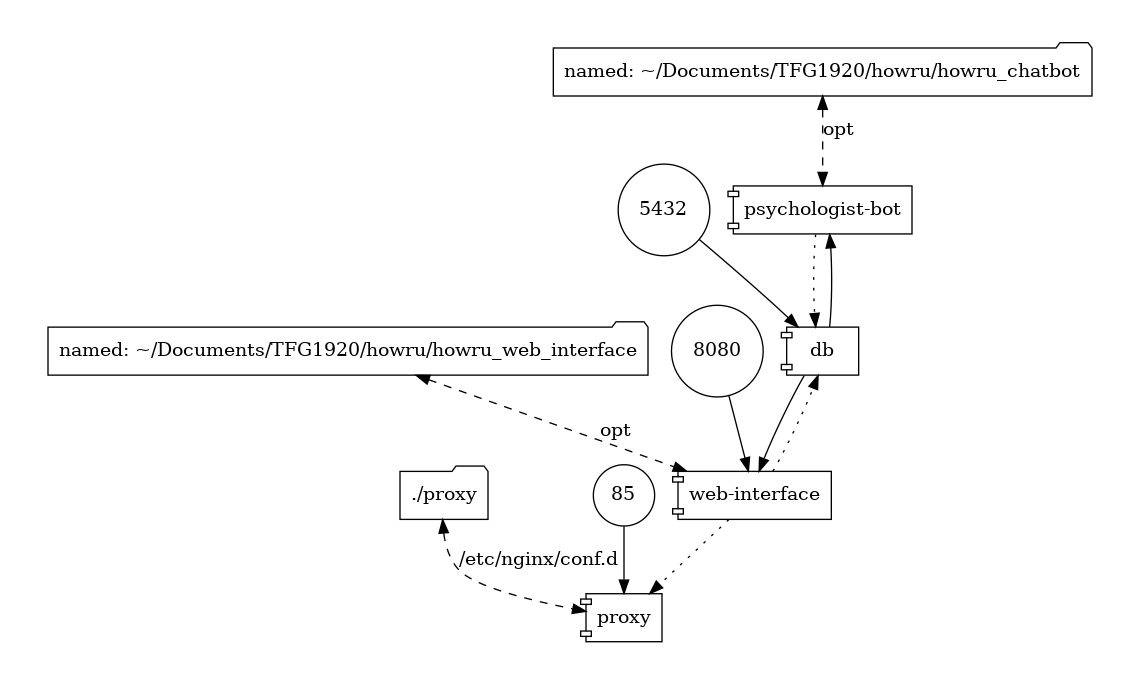
\includegraphics[width=\textwidth]{docker-compose.png}
  \caption{Docker-compose file schema. Generated by \protect\cite{dockerviz}}
\end{figure}
\section{Environment setup}
\label{sec:env_setup}

\subsection{Development environment}

The development environment will be deployed using \cite{docker}. To do that, the user just needs to install \emph{Docker}, clone the code repository and run the attached script:

\begin{lstlisting}[language=bash, caption={Commands to install Docker}, captionpos=b, mathescape=false]
$> sudo apt-get update
$> sudo apt install apt-transport-https ca-certificates curl gnupg-agent software-properties-common
$> curl -fsSL https://download.docker.com/linux/ubuntu/gpg | sudo apt-key add -
$> sudo add-apt-repository  "deb [arch=amd64] https://download.docker.com/linux/ubuntu $(lsb_release -cs) stable"
$> sudo apt update
$> sudo apt install docker-ce docker-ce-cli containerd.io
\end{lstlisting}

After that, the user needs to log out and back in so that permissions are re-evaluated. After that, the HOW-R-U development environment can be run by typing the following commands:

\begin{lstlisting}[mathescape=false, language=bash, caption={Commands to deploy development environment}, captionpos=b]
  $> git clone https://github.com/csp98/TFG1920
  $> cd howru/docker
  $> ./start.sh
\end{lstlisting}

The \emph{start.sh} scripts build all the images and then launches them in \emph{docker}:

\begin{lstlisting}[language=bash, caption={start.sh script}, captionpos=b]
#!/bin/zsh
# Chatbot
docker build -t psychologist-bot chatbot

# Web interface
docker build -t web_interface web_interface
docker build -t proxy proxy

docker-compose -p "howru" up -d --remove-orphans --force-recreate
\end{lstlisting}

\newpage
\subsection{Production environment}

The production environment will be deployed using \emph{Amazon Web Services}. There will be three tipes of instances: psychologist bot, web interface and databases.

\subsubsection{Pre-deployment: Telegram bot creation}

The first step is to create the production conversational agent in Telegram. To do so, the user must establish a conversation with \emph{@BotFather} and send the bot creation commands:

\begin{figure}[H]
  \centering
  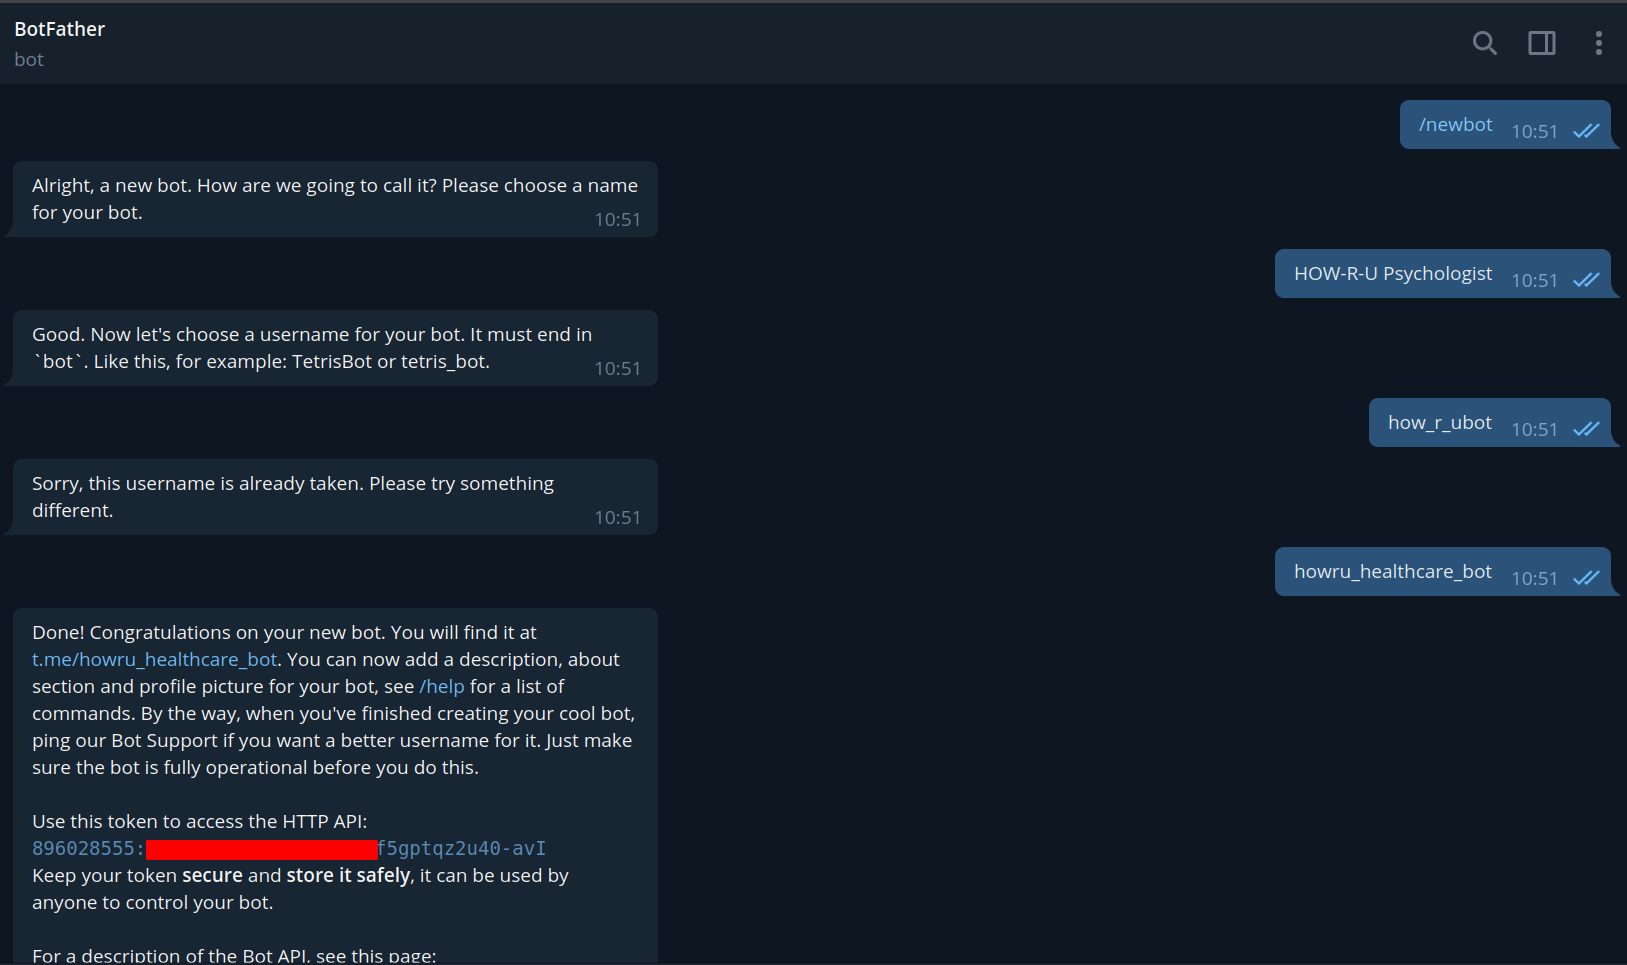
\includegraphics[width=\textwidth]{bot_creation.png}
  \caption{Telegram bot creation.}
\end{figure}

\emph{@BotFather} will provide the user with a private authentication token that HOW-R-U will use to control the conversational agent. The user can customize the bot by adding a profile picture, changing description, etc., by using the related \emph{@BotFather} commands.

\subsubsection{System deployment}

The next step is to deploy the system into Amazon Web Services \cite{aws}. The first component that is going to be deployed will be the database.

The user has to log in into \emph{Amazon Relational Database System (RDS)} and create a PostgreSQL database, setting an username and password. The user can use this tutorial as reference: \href{https://aws.amazon.com/getting-started/tutorials/create-connect-postgresql-db/}{https://aws.amazon.com/getting-started/tutorials/create-connect-postgresql-db/}.


\begin{figure}[H]
  \centering
  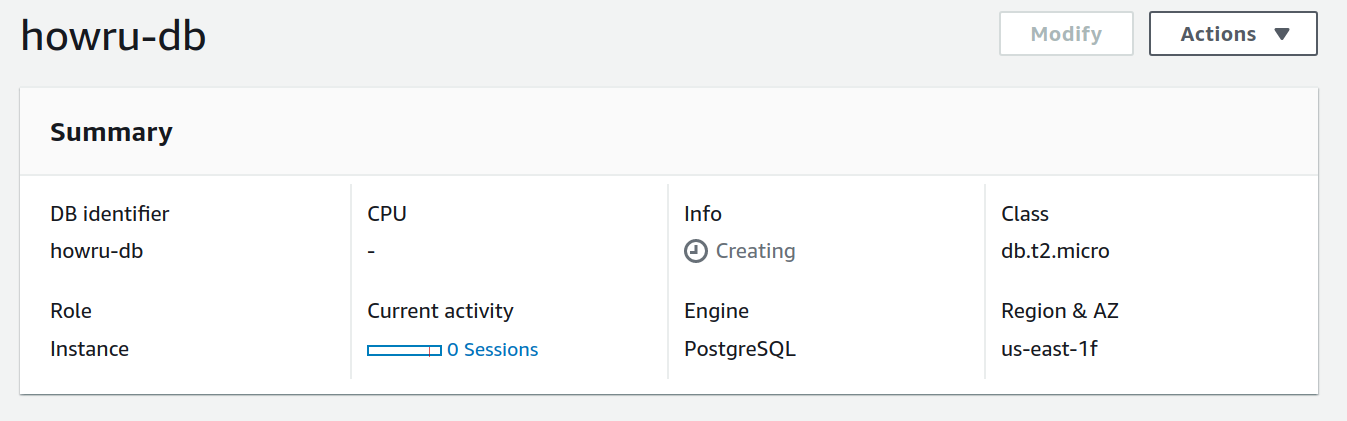
\includegraphics[width=\textwidth]{db_creation.png}
  \caption{Database instance being created.}
\end{figure}

Then, the chatbot and web interface instances should be created using EC2. They should work under a Linux distribution. The web interface needs an specific rule in the security group so that it can be accessed from outside (port 80, HTTP):

\begin{figure}[H]
  \centering
  
\includegraphics[width=0.9\textwidth]{web_int_sg.png}
  \caption{Security group rule for web interface instance.}
\end{figure}

The next step is to deploy the web interface. To do so, the user must clone the repository from the instance:

\begin{lstlisting}[mathescape=false, language=bash, caption={Commands to download the web interface repository}, captionpos=b]
  web_interface > sudo su
  web_interface > yum install git
  web_interface > mkdir /opt/web_interface
  web_interface > cd /opt/web_interface
  web_interface > git clone --recurse-submodules https://github.com/csp98/howru_web_interface.git .
\end{lstlisting}

Now we should configure four parameters: DB routes file, debug mode (should be disabled), allowed hosts and Django secret key. The first one consists of creating a file (\emph{/etc/howru/cfg/routes.json}) with the following content:

\begin{lstlisting}[caption={Routes file}, captionpos=b]
{
  "host": "<DB instance DNS>",
  "port": 5432,
  "name": "postgres",
  "user": "<DB username>",
  "password": "<DB password>"
}
\end{lstlisting}

The Django secret key can be generated with the following website: \\\href{https://miniwebtool.com/django-secret-key-generator/}{https://miniwebtool.com/django-secret-key-generator/}. Once retrieved, the user should create the following file:

\begin{lstlisting}[mathescape=false, language=bash, caption={Command to create Django key file and key.py file contents}, captionpos=b]
  web_interface > nano /opt/web_interface/core/key.py
  **********************
  KEY = '<KEY>'
  **********************
\end{lstlisting}

Finally, the user must edit \emph{/opt/web\_interface/core/settings.py} setting \emph{DEBUG=False} and \emph{ALLOWED\_HOSTS = ['*']}

The environment files are now ready. The next steps consist on installing \emph{Python}, the requirements and running the server.

\begin{lstlisting}[mathescape=false, language=bash, caption={Commands to install Python and its requirements}, captionpos=b]
web_interface > yum install python3 python3-pip python-psycopg2 postgresql gcc python3-devel
web_interface > pip3 install -r requirements.txt
web_interface > python3 manage.py makemigrations
web_interface > python3 manage.py migrate
\end{lstlisting}

Finally, we will configure \emph{screen} to detach the session where the interface will run:

\begin{lstlisting}[mathescape=false, language=bash, caption={Commands to detatch the session and run the web interface server}, captionpos=b]
web_interface > yum install screen
web_interface > screen
web_interface > python3 manage.py runserver 0:80
\end{lstlisting}

And finally press \emph{Ctrl+A+D} and close the SSH session. The web interface is now successfully configured and deployed and doctors can now use it by accessing through the public DNS.

Finally, let's deploy the conversational agent. Log in into the instance via SSH and do the following:

\begin{lstlisting}[mathescape=false, language=bash, caption={Commands to download HOW-R-U chatbot module and install its dependencies}, captionpos=b]
conv_agent > sudo su
conv_agent > yum install python3 python3-pip python3-devel git screen
conv_agent > mkdir /opt/chatbot
conv_agent > cd /opt/chatbot
conv_agent > git clone --recurse-submodules https://github.com/csp98/howru_chatbot.git .
\end{lstlisting}

Create the routes file (same as the web interface one) in the same directory. After that, the file with the bot secret token, \emph{/opt/chatbot/config/bot\_config.py}, and add the following:
\begin{python}[caption={bot\_config.py file contents}, captionpos=b]
TOKEN = "<SECRET TOKEN>"
\end{python}

Now install the requirements, detach the screen and launch the conversational agent:

\begin{lstlisting}[mathescape=false, language=bash, caption={Commands to detatch the screen, install the chatbot requirements and run it}, captionpos=b]
conv_agent > python3 -m pip install -r requirements.txt
conv_agent > screen
conv_agent > export PYTHONPATH=`pwd`
conv_agent > export DJANGO_SETTINGS_MODULE="manage.settings"
conv_agent > python3 manage.py makemigrations
conv_agent > python3 manage.py migrate
conv_agent > python3 src/bot.py
\end{lstlisting}

After that, HOW-R-U system is ready to be used.

\begin{figure}[H]
  \centering
    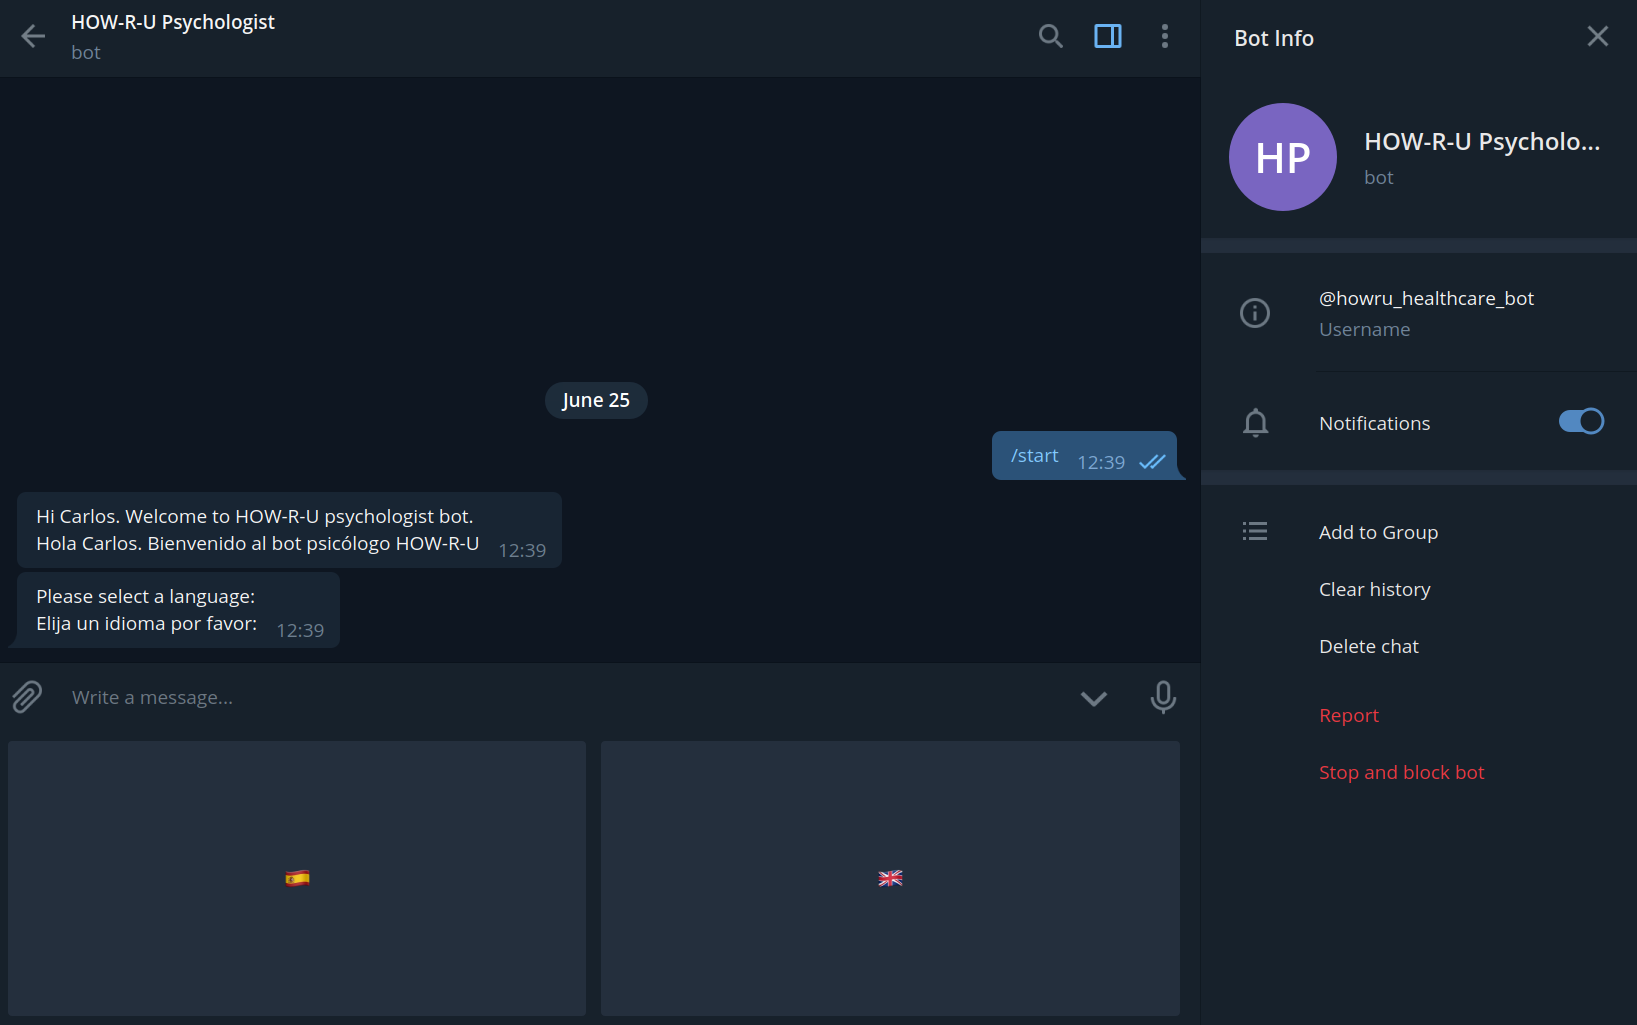
\includegraphics[width=\textwidth]{production.png}
    \caption{HOW-R-U production conversational agent.}
\end{figure}


\section{Discussion}

The discussion of the proposed system will be based on a SWOT analysis (\textbf{S}trengths, \textbf{W}eaknesses, \textbf{O}pportunities and \textbf{T}hreats). The main \underline{strength} of HOW-R-U is its versatility: it can be used in many different scenarios, from health domains to analysis of data based on surveys. For example, a health clinic could offer a suite of e-coaches based on HOW-R-U: a nutritionist, a psychologist, a dermatologyst, etc., that would make the patients regular questions so that their daily status is tracked by doctors, obtaining a big quantity of useful data.  Moreover, the interface is intended to be easy to use and learn so that users do not struggle when manipulating it. Another strength is that the patient does not need to install a specific application to use it because HOW-R-U conversational agent can be used both through Telegram Web or Desktop. Regarding the \underline{opportunities} of the system, a strong case of use could be a wide data analysis about COVID-19 symptoms to identify patterns over the population, build a map based on infected patients, etc.,. Furthermore, as Telegram is one of the chat applications that offers more privacy for its users, the system can be more attractive to them than other systems that use other apps ensuring less privacy.


The main \underline{weakness} of the system is that its deployment requires specific knowledge about architectures, system shells, etc., so it is not suitable for everyone. In addition,  Telegram is not used by the majority of people, so it is likely that most patients will have to install it. This weakness leads to the  \underline{threat} of another system that uses its own specific app. As patients would have to install an application in both cases, maybe they could opt for the particular one, that could offer another user interface, animations, etc.,. Another threat is that elderly people may not know how to use Telegram. Lastly, not every patient has a smartphone, so a minor percentage of the could not use the system.

\begin{figure}[H]
  \centering
    \begin{tcbraster}[raster columns=2, boxrule=0mm, arc=0mm]
  \begin{tcolorbox}[equal height group=A, size=fbox, colback=swotS!60, colframe=swotS!80!black, title=\textsc{strengths}]
  \begin{enumerate}
  \item Different scenarios.
  \item Multiple e-coaches.
  \item Intuitive interface.
  \item No extra software for patients.
  \end{enumerate}
  \end{tcolorbox}
  \begin{tcolorbox}[equal height group=A, size=fbox, colback=swotW!60, colframe=swotW!80!black, title=\textsc{weaknesses}]
  \begin{enumerate}
  \item Telegram is not used by the majority of people.
  \item System deployment requires knowledge on computer science.
  \end{enumerate}
  \end{tcolorbox}
  \begin{tcolorbox}[equal height group=B, size=fbox, colback=swotO!60, colframe=swotO!80!black, title=\textsc{opportunities}]
  \begin{enumerate}
  \item COVID-19 data analysis.
  \item Telegram ensures privacy.
  \end{enumerate}
  \end{tcolorbox}
  \begin{tcolorbox}[equal height group=B, size=fbox, colback=swotT!60, colframe=swotT!80!black, title=\textsc{threats}]
  \begin{enumerate}
  \item Elderly people may not know how to use Telegram.
  \item If patients do not have Telegram installed, they could install a specific app instead of Telegram.
  \item Not all patients have smartphones.
  \end{enumerate}
  \end{tcolorbox}
  \end{tcbraster}
  \caption{HOW-R-U SWOT analysis. Based on \href{http://www.mostlycolor.ch/2015/07/swot-matrices-in-latex.html}{http://www.mostlycolor.ch/2015/07/swot-matrices-in-latex.html}}
\end{figure}

\section{Planification and budget}

\subsection{Planification}

The planification of this project has been divided into two main groups: documentation and system implementation. The first part refers to the build process of this memory, along with learning to code it in \LaTeX \cite{latex}, whereas the second part consists on the process of learning to use the different frameworks that compose HOW-R-U to create it.

\begin{figure}[H]
    \makebox[\linewidth]{
\begin{ganttchart}[%Specs
     x unit = 1.3cm,  %<---------------------- New x unit
     y unit title= 1 cm,
     y unit chart=0.7cm,
     vgrid, hgrid,
     title height=1,
%     title/.style={fill=none},
     title label font=\bfseries\footnotesize,
     bar/.style={fill=blue},
     bar height=0.7,
     progress label text={},
     group right shift=0,
     group top shift=0.7,
     group height=.3,
     group peaks width={0.2},
     group label node/.append style={left=.3cm, font=\bfseries\scriptsize},
     bar label node/.append style={left=.3cm, font=\scriptsize},
     inline]{1}{9}
    %labels

    \gantttitle[]{2019}{2}
    \gantttitle[]{2020}{7}\\
    \gantttitle{Nov}{1}
    \gantttitle{Dec}{1}
    \gantttitle{Jan}{1}
    \gantttitle{Feb}{1}
    \gantttitle{Mar}{1}
    \gantttitle{Apr}{1}
    \gantttitle{May}{1}
    \gantttitle{Jun}{1}
    \gantttitle{Jul}{1}\\

    % Setting group if any
    \ganttgroup[inline=false, progress label text={}]{Documentation}{1}{9}\\
    \ganttbar[progress=100,inline=false]{Introduction}{1}{2}\\
    \ganttbar[progress=100,inline=false]{State of the art study}{1}{4}\\
    \ganttbar[progress=100,inline=false]{Architecture design}{4}{4}\\
    \ganttbar[progress=100,inline=false]{Implementation}{7}{8}\\
    \ganttbar[progress=100,inline=false]{Discussion and conclussions}{8}{9}\\
    \ganttbar[progress=100,inline=false]{Planification and budget}{9}{9}\\
    \ganttgroup[inline=false]{System implementation}{1}{9}\\
    \ganttbar[progress=100,inline=false, bar/.style={fill=green}]{Conversational agent}{5}{6}\\
    \ganttbar[progress=100,inline=false, bar/.style={fill=green}]{Web interface}{5}{6}\\
    \ganttbar[progress=100,inline=false, bar/.style={fill=green}]{Development environment (Docker)}{5}{5}\\
    \ganttbar[progress=100,inline=false, bar/.style={fill=green}]{Production environment (AWS)}{8}{8}\\
    \ganttbar[progress=100,inline=false, bar/.style={fill=green}]{Testing and bugfixing}{6}{8}\\
\end{ganttchart}
}
\caption{Gantt Diagram showing the project's planification time.}
\end{figure}

\subsubsection{Budget}

HOW-R-U is distributed under a Creative Commons “Attribution-NonCommercial-ShareAlike 4.0 International” license, which means that the project can be freely used \textbf{as long as} it is not used to generate profit, so the main budget element will be the hosting. HOW-R-U can be hosted in a propietary infrastructure (in which the system administrator would have to buy and maintain all the equipment) or in the cloud (where the system administrator would pay per use). Regarding the cloud model, there could be three approaches depending on the system usage: a high and scalable one, a low and non scalable one and a single instance.

\subsubsection{Scalable environment}

Scalable configuration is suitable if the system is widely used. It is formed by three tipes of instances, one per module: database, web interface and conversational agent. All these machines must be able to do autoscaling, (the number of machines increases and decreases according to the workload).

\begin{figure}[H]
  \centering
  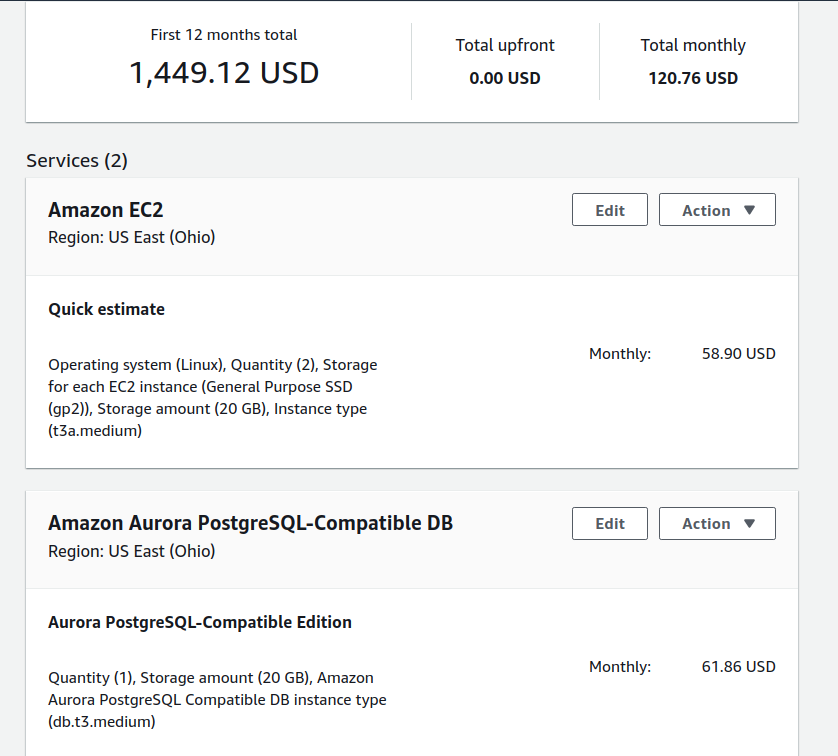
\includegraphics[width=0.5\textwidth]{cost.png}
  \caption{AWS cost for a HOW-R-U scalable production environment (Amazon Web Services Calculator (\href{https://calculator.aws/\#/estimate}{https://calculator.aws/\#/estimate}))}
\end{figure}

\begin{figure}[H]
  \centering
  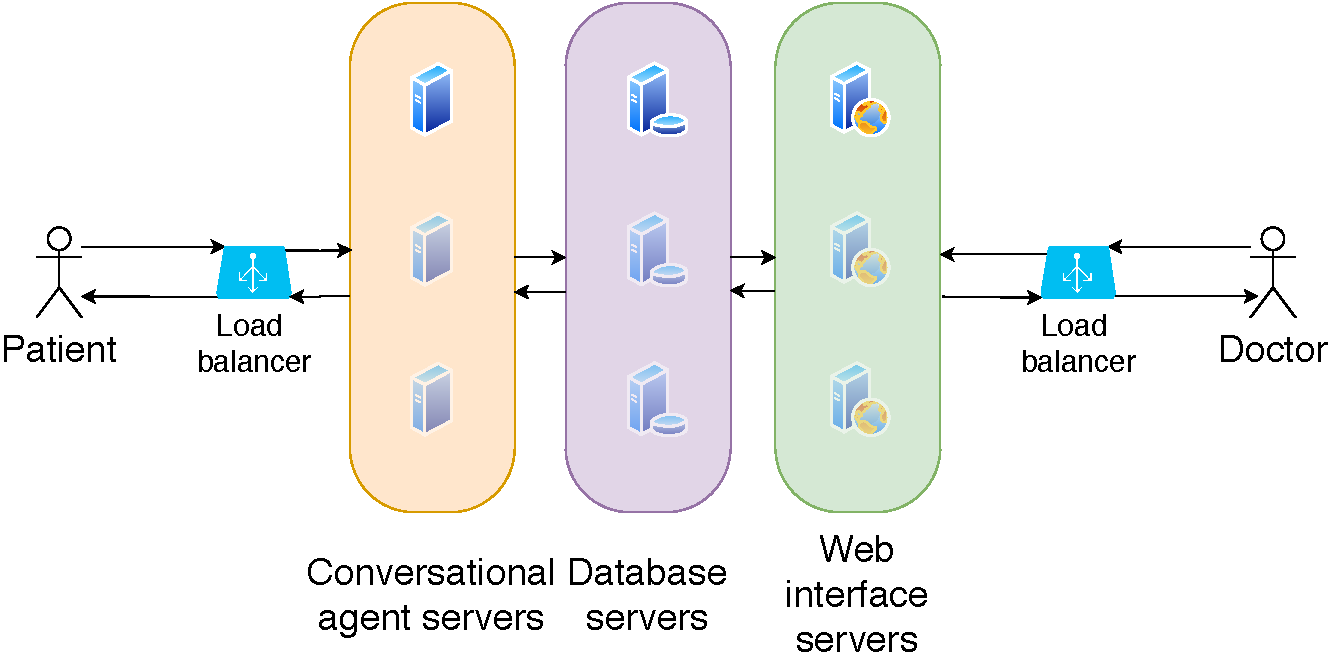
\includegraphics[width=0.7\textwidth]{scalable.pdf}
  \caption{Scalable environment architecture diagram. Created using \emph{diagrams.net} \protect\cite{drawio}.}
\end{figure}

\subsubsection{Non scalable environment}

Non-scalable configuration is oriented for environments where the workload is not high. It consists on two elements: a database cluster (which is scalable) and an instance that will host both the conversational agent and the web interface. If the number of accesses to the system increases, it would be easy to create another instance and transition to the scalable environment. Moreover, no database migrations would be needed, as this architecture provides an independent database cluster.

\begin{figure}[H]
  \centering
  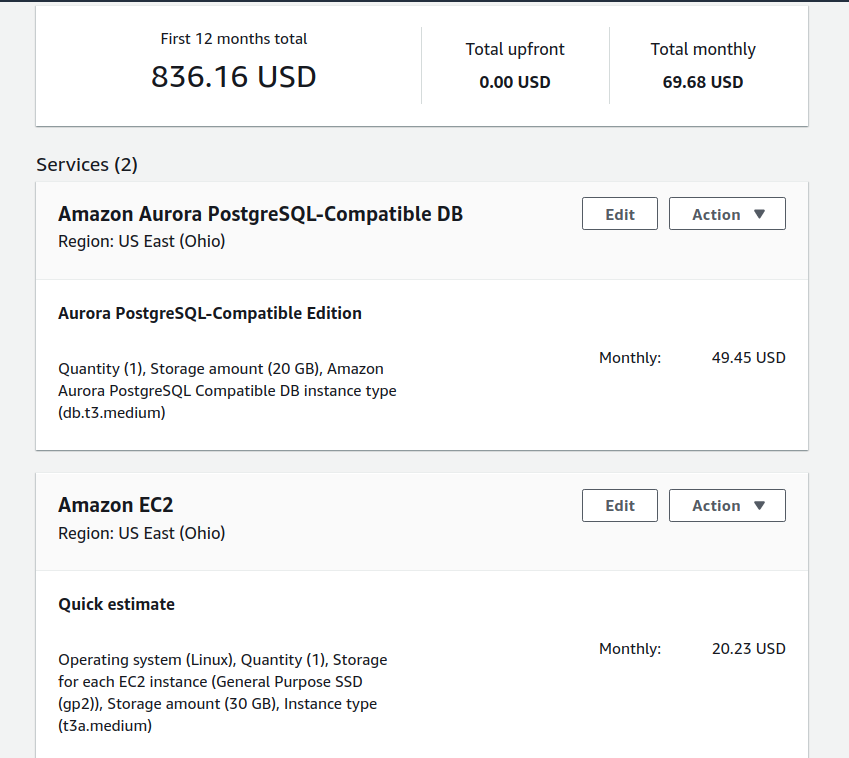
\includegraphics[width=0.65\textwidth]{cost_noscalable.png}
  \caption{AWS cost for a HOW-R-U non-scalable production environment (Amazon Web Services Calculator (\href{https://calculator.aws/\#/estimate}{https://calculator.aws/\#/estimate}))}
\end{figure}

\begin{figure}[H]
  \centering
  \includegraphics[width=0.7\textwidth]{non-scalable.pdf}
  \caption{Non-scalable environment architecture diagram. Created using \emph{diagrams.net} \protect\cite{drawio}.}
\end{figure}
\newpage

\subsubsection{One single instance}

This is the cheapest alternative, but the worst one if the system expects to get a high workload. It consists on a single instance where all modules run: database, web interface and conversational agent. Appart from the performance, the main disadvantage of this setup is that if the administrator wanted to switch to a scalable one it would be necessary to perform a database migration.

\begin{figure}[H]
  \centering
  \includegraphics[width=0.65\textwidth]{cost_one.png}
  \caption{AWS cost for a HOW-R-U one-instance production environment (Amazon Web Services Calculator (\href{https://calculator.aws/\#/estimate}{https://calculator.aws/\#/estimate}))}
\end{figure}

\begin{figure}[H]
  \centering
  \includegraphics[width=0.7\textwidth]{one-instance.pdf}
  \caption{One-instance environment architecture diagram. Created using \emph{diagrams.net} \protect\cite{drawio}.}
\end{figure}
\newpage

Another important element in the budget is the development cost of the system per employee which would be the following:

\begin{table}[h!]
  \centering
  \begin{tabular}{|c|c|}
    \hline
    \textbf{Concept} & \textbf{Cost} \\
    \hline
    Base salary & 1000\euro \\
    Bonus payments & 200\euro \\
    Proportional part of the extra pays & 150\euro \\
    Type of contract & Indefinite \\
    Type of working days & Full time \\
    Tax withholdings & 7\% \\
    Accident and occupational disease contribution basis & 1\% \\
    \hline
     \textbf{Total cost for the company} & 1767.15\euro \\
      \textbf{Net salary for the employee} & 1169.78\euro \\
    \hline
  \end{tabular}
  \caption{System cost per employee per month}
\end{table}

The total cost of the system (human resources and hosting) having one single employee is detailed below, depending on the chosen architecture:

\begin{table}[h!]
  \centering
  \begin{tabular}{|c|c|c|c|}
    \hline
    \textbf{Architecture} & \textbf{Human resources cost} & \textbf{Architecture cost} & \textbf{Total cost}\\
    \hline
     Scalable & 1767.15\euro & 107.42\euro & 1874.57\euro \\
     Non scalable & 1767.15\euro & 62\euro & 1829.15\euro \\
     One instance & 1767.15\euro & 44.44\euro & 1811.59\euro \\
     \hline
  \end{tabular}
  \caption{System total cost per moth}
\end{table}
\newpage
\section{Conclusions}

The sections below analyse the project's success level, regarding every goal defined in the \hyperref[sec:objectives]{Objectives section}, as well as possible areas for potential future work.

\subsection{Achievements}

\begin{itemize}
  \item \textbf{Main goal: to develop a conversational-agent-as-a-sensor which will be able to interact with a person with a disorder and ask questions defined by specialists}. This objective is achieved, as the conversational agent module manages patient-system interactions. Moreover, the system allows doctors to create custom questions through the web interface. In addition, they can use questions created by other specialists (if they set them as public).
  \item \textbf{Secondary goals}
  \begin{itemize}
    \item \textbf{To design a graphical web interface where doctors can consult their patient’s responses}. This goal is also reached, as shown in the \hyperref[sec:web_int]{web interface implementation section}. Besides, doctors can either analyse the retrieved data through the integrated charts or download a CSV file to ellaborate their own metrics.
    \item \textbf{To design a flexible and scalable architecture to add functionality to the system}. As doctors can add custom questions with the system, HOW-R-U can be used in a lot of scenarios. The \emph{data analyst} feature also allows the system to be used not only in medical situations, but also in survey ones.
    \item \textbf{To design an architecture based on containers to host the different system modules}. As shown in the \hyperref[sec:docker]{Docker implementation section}, the system is structured in containers so that a development environment can be easily set up.
    \item \textbf{To implement a system that covers the previous goals}. As the \hyperref[sec:implementation]{implementation} section illustrates, the proposed system has been successfully developed.
    \item \textbf{To test a beta version of the assistant in real people and analyse the retrieved data as well as target audience’s feelings about it}. This is the only objective that has not been accomplished. HOW-R-U started being a much more elementary system: it did not have a web interface (doctors would have had to control everything from another Telegram bot), questions were not customizable (the developer would have had to define and hardcode them), there were no concepts such as frequency or priority (questions were asked daily in a random order), etc.,.
    We decided to leave this goal behind in order to give more functionality and customization to HOW-R-U so that it could be used in a wider variety of scenarios, not only the health care ones.
  \end{itemize}
\end{itemize}
\newpage
\subsection{Future work}

HOW-R-U functionality can be extended in many ways. For example, the web interface could be enriched with more data views, like patient's country, city, age, etc. Moreover, this module could be able to automatically generate the charts requested by the user. Another improvement area can be the conversational agent module, which could be ported to other chat applications in order to cover more population. This would make patients feel more confortable about HOW-R-U, as they would not have to download another chat application if they did not have \cite{Telegram} installed.


Another area of improvement could be the development of a QA (Quality Assurance) suite of tests. This would make easier to detect if a new change performed in the system introduces regression over the previous status of HOW-R-U. What is more, HOW-R-U could be analyzed in order to apply profiling techniques to improve the system performance by detecting the bottleneck points of the different flows and optimising them. Finally, the system could be translated to other languages so that it can be used worldwide. This requirement would also need more timezones to be available in order to correctly work with patients' schedule.
\vspace{1cm}

The whole source code of HOW-R-U is available at \href{https://github.com/csp98/TFG1920}{https://github.com/csp98/TFG1920}

\newpage
\bibliographystyle{apacite}
\bibliography{refs}
\doclicenseThis

\end{document}
